%==============================================================================
% tento soubor pouzijte jako zaklad
% this file should be used as a base for the thesis
% Autoři / Authors: 2008 Michal Bidlo, 2019 Jaroslav Dytrych
% Kontakt pro dotazy a připomínky: sablona@fit.vutbr.cz
% Contact for questions and comments: sablona@fit.vutbr.cz
%==============================================================================
% kodovani: UTF-8 (zmena prikazem iconv, recode nebo cstocs)
% encoding: UTF-8 (you can change it by command iconv, recode or cstocs)
%------------------------------------------------------------------------------
% zpracování / processing: make, make pdf, make clean
%==============================================================================
% Soubory, které je nutné upravit nebo smazat: / Files which have to be edited or deleted:
%   projekt-20-literatura-bibliography.bib - literatura / bibliography
%   projekt-01-kapitoly-chapters.tex - obsah práce / the thesis content
%   projekt-01-kapitoly-chapters-en.tex - obsah práce v angličtině / the thesis content in English
%   projekt-30-prilohy-appendices.tex - přílohy / appendices
%   projekt-30-prilohy-appendices-en.tex - přílohy v angličtině / appendices in English
%==============================================================================
\documentclass[]{fitthesis} % bez zadání - pro začátek práce, aby nebyl problém s překladem
%\documentclass[english]{fitthesis} % without assignment - for the work start to avoid compilation problem
%\documentclass[zadani]{fitthesis} % odevzdani do wisu a/nebo tisk s barevnými odkazy - odkazy jsou barevné
%\documentclass[english,zadani]{fitthesis} % for submission to the IS FIT and/or print with color links - links are color
%\documentclass[zadani,print]{fitthesis} % pro černobílý tisk - odkazy jsou černé
%\documentclass[english,zadani,print]{fitthesis} % for the black and white print - links are black
%\documentclass[zadani,cprint]{fitthesis} % pro barevný tisk - odkazy jsou černé, znak VUT barevný
%\documentclass[english,zadani,cprint]{fitthesis} % for the print - links are black, logo is color
% * Je-li práce psaná v anglickém jazyce, je zapotřebí u třídy použít 
%   parametr english následovně:
%   If thesis is written in English, it is necessary to use 
%   parameter english as follows:
%      \documentclass[english]{fitthesis}
% * Je-li práce psaná ve slovenském jazyce, je zapotřebí u třídy použít 
%   parametr slovak následovně:
%   If the work is written in the Slovak language, it is necessary 
%   to use parameter slovak as follows:
%      \documentclass[slovak]{fitthesis}
% * Je-li práce psaná v anglickém jazyce se slovenským abstraktem apod., 
%   je zapotřebí u třídy použít parametry english a enslovak následovně:
%   If the work is written in English with the Slovak abstract, etc., 
%   it is necessary to use parameters english and enslovak as follows:
%      \documentclass[english,enslovak]{fitthesis}

% Základní balíčky jsou dole v souboru šablony fitthesis.cls
% Basic packages are at the bottom of template file fitthesis.cls
% zde můžeme vložit vlastní balíčky / you can place own packages here

% Kompilace po částech (rychlejší, ale v náhledu nemusí být vše aktuální)
% Compilation piecewise (faster, but not all parts in preview will be up-to-date)
% \usepackage{subfiles}

% Nastavení cesty k obrázkům
% Setting of a path to the pictures
%\graphicspath{{obrazky-figures/}{./obrazky-figures/}}
%\graphicspath{{obrazky-figures/}{../obrazky-figures/}}

%---rm---------------
\renewcommand{\rmdefault}{lmr}%zavede Latin Modern Roman jako rm / set Latin Modern Roman as rm
%---sf---------------
\renewcommand{\sfdefault}{qhv}%zavede TeX Gyre Heros jako sf
%---tt------------
\renewcommand{\ttdefault}{lmtt}% zavede Latin Modern tt jako tt

% vypne funkci šablony, která automaticky nahrazuje uvozovky,
% aby nebyly prováděny nevhodné náhrady v popisech API apod.
% disables function of the template which replaces quotation marks
% to avoid unnecessary replacements in the API descriptions etc.
\csdoublequotesoff



\usepackage{url}
\usepackage{placeins}
\usepackage{hyperref}

% =======================================================================
% balíček "hyperref" vytváří klikací odkazy v pdf, pokud tedy použijeme pdflatex
% problém je, že balíček hyperref musí být uveden jako poslední, takže nemůže
% být v šabloně
% "hyperref" package create clickable links in pdf if you are using pdflatex.
% Problem is that this package have to be introduced as the last one so it 
% can not be placed in the template file.
\ifWis
\ifx\pdfoutput\undefined % nejedeme pod pdflatexem / we are not using pdflatex
\else
  \usepackage{color}
  \usepackage[unicode,colorlinks,hyperindex,plainpages=false,pdftex]{hyperref}
  \definecolor{hrcolor-ref}{RGB}{223,52,30}
  \definecolor{hrcolor-cite}{HTML}{2F8F00}
  \definecolor{hrcolor-urls}{HTML}{092EAB}
  \hypersetup{
	linkcolor=hrcolor-ref,
	citecolor=hrcolor-cite,
	filecolor=magenta,
	urlcolor=hrcolor-urls
  }
  \def\pdfBorderAttrs{/Border [0 0 0] }  % bez okrajů kolem odkazů / without margins around links
  \pdfcompresslevel=9
\fi
\else % pro tisk budou odkazy, na které se dá klikat, černé / for the print clickable links will be black
\ifx\pdfoutput\undefined % nejedeme pod pdflatexem / we are not using pdflatex
\else
  \usepackage{color}
  \usepackage[unicode,colorlinks,hyperindex,plainpages=false,pdftex,urlcolor=black,linkcolor=black,citecolor=black]{hyperref}
  \definecolor{links}{rgb}{0,0,0}
  \definecolor{anchors}{rgb}{0,0,0}
  \def\AnchorColor{anchors}
  \def\LinkColor{links}
  \def\pdfBorderAttrs{/Border [0 0 0] } % bez okrajů kolem odkazů / without margins around links
  \pdfcompresslevel=9
\fi
\fi
% Řešení problému, kdy klikací odkazy na obrázky vedou za obrázek
% This solves the problems with links which leads after the picture
\usepackage[all]{hypcap}

% Informace o práci/projektu / Information about the thesis
%---------------------------------------------------------------------------
\projectinfo{
  %Prace / Thesis
  project={BP},            %typ práce BP/SP/DP/DR  / thesis type (SP = term project)
  year={2020},             % rok odevzdání / year of submission
  date=\today,             % datum odevzdání / submission date
  %Nazev prace / thesis title
  title.cs={Rozpoznávání postojů z filmových recenzí},  % název práce v češtině či slovenštině (dle zadání) / thesis title in czech language (according to assignment)
  title.en={Sentiment Analysis from Movie Reviews}, % název práce v angličtině / thesis title in english
  %title.length={14.5cm}, % nastavení délky bloku s titulkem pro úpravu zalomení řádku (lze definovat zde nebo níže) / setting the length of a block with a thesis title for adjusting a line break (can be defined here or below)
  %sectitle.length={14.5cm}, % nastavení délky bloku s druhým titulkem pro úpravu zalomení řádku (lze definovat zde nebo níže) / setting the length of a block with a second thesis title for adjusting a line break (can be defined here or below)
  %Autor / Author
  author.name={Daniel},   % jméno autora / author name
  author.surname={Bílý},   % příjmení autora / author surname 
  %author.title.p={Bc.}, % titul před jménem (nepovinné) / title before the name (optional)
  %author.title.a={Ph.D.}, % titul za jménem (nepovinné) / title after the name (optional)
  %Ustav / Department
  department={UPGM}, % doplňte příslušnou zkratku dle ústavu na zadání: UPSY/UIFS/UITS/UPGM / fill in appropriate abbreviation of the department according to assignment: UPSY/UIFS/UITS/UPGM
  % Školitel / supervisor
  supervisor.name={Pavel},   % jméno školitele / supervisor name 
  supervisor.surname={Smrž},   % příjmení školitele / supervisor surname
  supervisor.title.p={doc. RNDr.},   %titul před jménem (nepovinné) / title before the name (optional)
  supervisor.title.a={Ph.D.},    %titul za jménem (nepovinné) / title after the name (optional)
  % Klíčová slova / keywords
  keywords.cs={Analýza sentimentu, stahování dat z webu, strojové učení, filmové recenze}, % klíčová slova v českém či slovenském jazyce / keywords in czech or slovak language
  keywords.en={Sentiment analysis, web scraping, machine learning, movie reviews}, % klíčová slova v anglickém jazyce / keywords in english
  %keywords.en={Here, individual keywords separated by commas will be written in English.},
  % Abstrakt / Abstract
  abstract.cs={Tato práce je zaměřena na tvorbu systému, který je schopný pravidelně stahovat filmové recenze z webu a následně je analyzovat. Zdrojů recenzí je několik a to českých i anglických (čsfd, fdb, imdb a rotten tomatoes). Analýza sentimentu recenzí je prováděna za pomocí strojového učení. Výsledky analýz jsou zobrazovány ve webovém prohlížeči.}, % abstrakt v českém či slovenském jazyce / abstract in czech or slovak language
  abstract.en={This thesis is focused on creating a system which is capable of downloading movie reviews from the web and analysing them. There is several sources of movie reviews, czech and english (čsfd, fdb, imdb and rotten tomatoes). The sentiment analysis is performed using machine learning. Results of the analysis are shown in a browser.}, % abstrakt v anglickém jazyce / abstract in english
  %abstract.en={An abstract of the work in English will be written in this paragraph.},
  % Prohlášení (u anglicky psané práce anglicky, u slovensky psané práce slovensky) / Declaration (for thesis in english should be in english)
  declaration={Prohlašuji, že jsem tuto bakalářskou práci vypracoval samostatně pod vedením pana Doc. RNDr. Pavla Smrže, Ph.D. Uvedl jsem všechny literární prameny, publikace a další zdroje, ze kterých jsem čerpal.},
  %declaration={I hereby declare that this Bachelor's thesis was prepared as an original work by the author under the supervision of Mr. X
% The supplementary information was provided by Mr. Y
% I have listed all the literary sources, publications and other sources, which were used during the preparation of this thesis.},
 % TODO Poděkování (nepovinné, nejlépe v jazyce práce) / Acknowledgement (optional, ideally in the language of the thesis)
 % acknowledgment={V této sekci je možno uvést poděkování vedoucímu práce a těm, kteří poskytli odbornou pomoc
%(externí zadavatel, konzultant apod.).},
  %acknowledgment={Here it is possible to express thanks to the supervisor and to the people which provided professional help
%(external submitter, consultant, etc.).},
  % Rozšířený abstrakt (cca 3 normostrany) - lze definovat zde nebo níže / Extended abstract (approximately 3 standard pages) - can be defined here or below
  %extendedabstract={Do tohoto odstavce bude zapsán rozšířený výtah (abstrakt) práce v českém (slovenském) jazyce.},
  %faculty={FIT}, % FIT/FEKT/FSI/FA/FCH/FP/FAST/FAVU/USI/DEF
  faculty.cs={Fakulta informačních technologií}, % Fakulta v češtině - pro využití této položky výše zvolte fakultu DEF / Faculty in Czech - for use of this entry select DEF above
  faculty.en={Faculty of Information Technology}, % Fakulta v angličtině - pro využití této položky výše zvolte fakultu DEF / Faculty in English - for use of this entry select DEF above
  %department.cs={Ústav matematiky}, % Ústav v češtině - pro využití této položky výše zvolte ústav DEF nebo jej zakomentujte / Department in Czech - for use of this entry select DEF above or comment it out
  %department.en={Institute of Mathematics} % Ústav v angličtině - pro využití této položky výše zvolte ústav DEF nebo jej zakomentujte / Department in English - for use of this entry select DEF above or comment it out
}

% Rozšířený abstrakt (cca 3 normostrany) - lze definovat zde nebo výše / Extended abstract (approximately 3 standard pages) - can be defined here or above
%\extendedabstract{Do tohoto odstavce bude zapsán výtah (abstrakt) práce v českém (slovenském) jazyce.}

% nastavení délky bloku s titulkem pro úpravu zalomení řádku - lze definovat zde nebo výše / setting the length of a block with a thesis title for adjusting a line break - can be defined here or above
%\titlelength{14.5cm}
% nastavení délky bloku s druhým titulkem pro úpravu zalomení řádku - lze definovat zde nebo výše / setting the length of a block with a second thesis title for adjusting a line break - can be defined here or above
%\sectitlelength{14.5cm}

% řeší první/poslední řádek odstavce na předchozí/následující stránce
% solves first/last row of the paragraph on the previous/next page
\clubpenalty=10000
\widowpenalty=10000

% checklist
\newlist{checklist}{itemize}{1}
\setlist[checklist]{label=$\square$}

\begin{document}
  % Vysazeni titulnich stran / Typesetting of the title pages
  % ----------------------------------------------
  \maketitle
  % Obsah
  % ----------------------------------------------
  \setlength{\parskip}{0pt}

  {\hypersetup{hidelinks}\tableofcontents}
  
  % Seznam obrazku a tabulek (pokud prace obsahuje velke mnozstvi obrazku, tak se to hodi)
  % List of figures and list of tables (if the thesis contains a lot of pictures, it is good)
  \ifczech
    \renewcommand\listfigurename{Seznam obrázků}
  \fi
  \ifslovak
    \renewcommand\listfigurename{Zoznam obrázkov}
  \fi
  % {\hypersetup{hidelinks}\listoffigures}
  
  \ifczech
    \renewcommand\listtablename{Seznam tabulek}
  \fi
  \ifslovak
    \renewcommand\listtablename{Zoznam tabuliek}
  \fi
  % {\hypersetup{hidelinks}\listoftables}

  \ifODSAZ
    \setlength{\parskip}{0.5\bigskipamount}
  \else
    \setlength{\parskip}{0pt}
  \fi

  % vynechani stranky v oboustrannem rezimu
  % Skip the page in the two-sided mode
  \iftwoside
    \cleardoublepage
  \fi

  % Text prace / Thesis text
  % ----------------------------------------------
  
  %TODO
  \chapter{Úvod}
\label{uvod}

Rozpoznávání postojů (také známé jako analýza sentimentu nebo dolování názorů) je soubor analytických technik, jejichž cílem je extrahovat subjektivní názor z textu. Obvykle se rozlišuje mezi pozitivním, negativním a někdy i neutrálním postojem autora.
Další možností je určování míry pozitivity názoru na předem definované stupnici (například často používaných jedna až pět hvězdiček). Tento úkol je samozřejmě obtížnější než prosté určování polarity. Už ze statistického hlediska je obtížnější určit správnou třídu z pěti než z pouhých dvou. Další komplikací je často nejasná hranice mezi jednotlivými třídami. 

Téma analýzy sentimentu je dnes velice populární. K popularitě dopomohlo množství nestrukturovaných dat, které jsou na webu k dispozici. Těchto dat se společnosti snaží co nejvíce využít, proto do takovýchto analyzátorů investují. Je možné nalézt mnoho komerčních analyzátorů, které nabízí své služby (\emph{Gavagai}\footnote{\url{https://www.gavagai.io/}}, \emph{Natural language API} od firmy Google\footnote{\url{https://cloud.google.com/}} nebo \emph{Brand24}\footnote{\url{https://brand24.com/}}.

Využívaným typem dat pro analýzu sentimentu se staly recenze a to především filmů a seriálů. Důvodem je jejich dostupnost (existují webové stránky specificky vytvořené pro recenze), množství (především filmových recenzí je nespočet) a fakt, že recenze jsou již ohodnoceny autorem (nemusí být manuálně anotovány). Právě z těchto důvodů se v práci snažím prozkoumat využitelnost klasifikátorů natrénovaných na těchto datech v jiných doménách. Dalším prozkoumaným faktorem je potřebné množství dat při trénování analyzátorů.

Tato práce má za cíl navrhnout a implementovat systém, který by byl schopný analyzovat texty filmových recenzí, a tím z nich získat názor autora k danému filmu či seriálu. Data získaná z analýzy by zpracoval a představil uživateli. Analýzu je možné provádět celou řadou metod, vybrané metody jsou tedy porovnány vzhledem k jejich přesnosti. 

Výsledkem práce by měl být systém, který napomůže společnostem točící filmy i zákazníkům, kteří je sledují.

Společnosti za použití tohoto systému mohou jednoduše analyzovat názory lidí na jejich práci. Nejenže zjistí celkový názor na produkt, ale také mají možnost filtrovat názory na různé aspekty tohoto produktu. Důležitou informací získanou tímto systémem je změna názoru na daný film či seriál v čase. Společnost například může po vytvoření marketingové kampaně sledovat její dopad na názory lidí, popřípadě včas zamezit nějakému fiasku.

Zákazníkům tento systém pomůže při hledání filmu, nebo seriálu, který by se jim mohl líbit. Dále by mohl napomáhat uživatelům s doplňováním \uv{hvězdičkového} hodnocení při dopsání nové recenze (obsah recenze a výsledné hodnocení uživatele se občas dost liší).  

Text práce se skládá z následujících částí. Kapitola \ref{teorie} nabízí pohled na teorii potřebnou k vytvoření tohoto systému. Prozkoumány jsou základní i pokročilé techniky analýzy sentimentu, možnosti získávání dat z webu, jejich uložení a techniky pro předzpracování dat. Kapitola \ref{navrh} využívá teorii k návrhu a kapitola \ref{implementace} k implementaci popisovaného systému. V kapitole \ref{vysledky} je vytvořený systém vyhodnocen. Aplikace běží na adrese \url{http://athena1.fit.vutbr.cz:8078/}. 
  \chapter{Rozbor řešené problematiky} 
\label{teorie}

Tato kapitola se věnuje teoretickému popisu jednotlivých částí systému. V průběhu jsou rozebírány i případné problémy, se kterými je potřeba se vypořádat. Jejich řešení je pouze nastíněno, samotná implementace je v kapitole \ref{implementace}. 

Prvním okruhem zájmu je způsob získávání dat z webu a jejich uložení. Dále se provede jejich analýza. Informace získané z analýzy je nutné také uložit a vhodným způsobem zobrazit uživateli (například jako tabulku nebo graf). Každému z těchto okruhů je věnována vlastní sekce. 

\section{Analýza sentimentu}
V této sekci chci rozebrat základní principy a metody analýzy sentimentu. Tato analýza se snaží v textu hledat názory uživatele a určit, jestli jsou pozitivní, negativní nebo neutrální. Názory se mohou týkat produktu, služby nebo například organizace jako celku, ale také jen jednotlivých částí. Analýza sentimentu se také zabývá extrakcí emocí z textu (hněv, radost, smutek). Názory jsou obvykle emocionálně zabarvené, to napomáhá je vyhledat. Emočně zbarvený text bude pravděpodobně obsahovat slova jako \uv{krásný} nebo \uv{příšerný}. Na základě tohoto faktu staví některé techniky analýzy. Objektivní komentáře typu \uv{Film je dlouhý 120 minut} nejsou pro tuhle analýzu zajímavé.

Výsledkem analýzy tedy může být polarita (pozitivní, negativní, popřípadě neutrální), někdy také doplněna intenzitou dané polarity (škála hodnot, například od 1 do 5).

Jak je popsáno v \cite{veselovska-2017}, analýza postoje se obecně dělí do třech úrovní. První analyzuje dokument jako celek (např. celý komentář), druhá úroveň je větní, která zjišťuje názor v~jednotlivých větách a třetí je na úrovni aspektu.
Analýza na každé z těchto úrovní obvykle vyžaduje trochu jiný přístup, některé metody analýzy jsou však využitelné na více úrovních. 

Analyzování na úrovni dokumentu je vhodné provádět pokud se celý dokument vyjadřuje k jedné entitě (v případě recenzí je to daný film). Analýza se provádí za předpokladu, že daný dokument obsahuje názor.

Na úrovni větní se zjišťuje jaký sentiment mají jednotlivé věty, to dává větší detail o~analyzovaném textu. Sloučením sentimentů jednotlivých vět je možné zjistit celkový sentiment dokumentu. Analýza na této úrovni souvisí s analýzou subjektivity, která rozpoznává objektivní věty od subjektivních (některé věty názor neobsahují a jak už bylo řečeno, objektivní věty nejsou pro analýzu zajímavé). Polarita názoru se tedy analyzuje až poté, co je věta označena za subjektivní. Objektivní věty se obvykle označují za neutrální. 

Analýza na úrovni aspektu sleduje názory na určité části dané věci. Například ve větě \uv{Herci byli skvělí, ale prostředí nic moc.} se vyskytují dva aspekty filmu. Herci, ti mají hodnocení pozitivní a prostředí, které má negativní. Analýza na úrovni aspektu se dělí na dva úkoly. Prvním je nalezení zmínky o hledaném aspektu a druhým je přiřazení polarity této zmínce.

Analyzovat postoj uživatele není jednoduchý úkol. Velkou problematiku přináší lidský jazyk, který je dosti volný a kontextový. Jedním z těchto problémů je rozpoznat ironii a~sarkasmus. 
Například z věty \uv{Tento film je opravdu výborný!} nelze poznat, jakým způsobem to autor myslel.
Jak popisuje \cite{filatova-2012-irony}, nejzásadnější komplikací je fakt, že ironie ani sarkasmus nejsou formálně definovány a nedají se lehce poznat (například sadou pravidel). Oba tyto fenomény jsou dynamické a vyvíjí se. Ironii a sarkasmus se dá částečně poznat podle některých ustálených frází, emotikonů nebo například otazníků a vykřičníků. Dalším pomocným faktem je, že ironie a sarkasmus se častěji využívají pro záporná hodnocení a často se objevují v podobném kontextu. Ocitovaná práce se problém sarkasmu a ironie snaží řešit vytvořením párů ironických a neironických recenzí ke stejnému produktu a jejich následnou analýzou.

Zde \cite{Ptcek2014SarcasmDO} tento problém řeší využitím klasifikátorů založených na metodě pomocných vektorů a maximální entropie. Klasifikátory jsou trénovány na datech ze sociální sítě \emph{Twitter}. V práci jsou prozkoumány různé metody předzpracování a extrakce příznaků, snaží se také zpracovat emotikony a interpunkční znaménka. Vytvořený systém detekuje ironii a~sarkasmus s F1 skóre 0.92 pro angličtinu a 0.58 pro češtinu. Tento rozdíl je způsobený velikostmi trénovacích datových sad (trénovací sada pro angličtinu je mnohem větší). Při zmenšení anglické datové sady na velikost české klesne F1 skóre klasifikátoru pro angličtinu pouze na 0.73, z toho vyplývá, že v českém jazyku je obtížnější detekovat ironii a sarkasmus.  

V následujících podsekcích rozebírám základní metody analýzy. Podle \cite{approaches} (práce byla využita pro základní informace o metodách) jsou přístupy založené na slovníku, pravidlech nebo strojovém učení.


\subsection{Metody využívající lexikon}
Základem metod je myšlenka, že celková polarita věty nebo dokumentu se dá zjistit z~polarit jednotlivých slov nebo frází. Má více možných implementací, obecně je však analýza založena na seznamu slov (frází), které jsou označeny polaritou a jejich intenzitou. Slovo \uv{děsný} by mělo například hodnotu -7 (polarita záporná s intenzitou 7). Naopak slovo \uv{úžasný} by mělo například hodnotu 6 (polarita kladná s intenzitou 6). 
Jakou polaritu a intenzitu by slova měly mít jsou problémy samy o sobě. Polarita je závislá na kontextu (\uv{malý pokoj v~hotelu} versus \uv{malá čekací doba}). Určení intenzity je zase silně subjektivní, každý má k určitým slovům různé asociace.

Například v \cite{lexikon} je tato metoda dále rozšířena o sledování intenzifikace (\uv{docela dobrý} versus \uv{velice dobrý}) a negace (\uv{je dobrý} versus \uv{není dobrý}). Takovýchto rozšíření této metody existuje celá řada.

Přesnost metody využívající lexikon je oproti ostatním metodám více závislá na správném předzpracování dat. Normalizace, lemmatizace a stematizace velice napomáhají v přiřazení slov z textu k těm, které se vyskytují v předem vytvořeném lexikonu.

Po sestavení dostatečně velkého lexikonu nejčastěji používaných slov se vezme analyzovaný text a všem slovům se přiřadí jejich hodnota z lexikonu. Slova bez polarity (předložky, spojky apod.) se v lexikonu nenachází. Poté se jen sečtou všechny hodnoty a tím vznikne výsledné hodnocení daného textu. Výsledná hodnota se vydělí počtem slov v textu. Tímto se celkové ohodnocení textu normalizuje a předejde se tomu, že by text byl pozitivnější jenom protože je delší. 

\subsection{Metody založené na pravidlech}
Podle definice v \cite{approaches}, metoda využívá člověkem předem definovaných pravidel. Nejprve se celý dokument rozdělí na slova. Poté se podle daných pravidel testuje přítomnost slov, které jsou opět uložené v lexikonu. Stejně jako u metody založené na lexikonu se připočítává celkové skóre dokumentu. Pokud je celkové skóre větší nebo rovno nula je dokument pozitivní, pokud menší než nula, je dokument negativní. Výstup analyzátoru se porovná se správnou odpovědí. Pokud v lexikonu analyzátoru chybí nějaká slova z textu, která by napomohla analýze, jsou přidána do lexikonu. Analyzátor je tak schopný učit se nová slova ze vstupního textu.

\subsection{Metody založené na strojovém učení}
\label{machinelearning}
Těchto metod opět existuje celá řada \cite{approaches} \cite{MEDHAT20141093}, každá s různými implementacemi. 
Základní myšlenka je vytvoření algoritmu, který je schopný ze vstupních dat vytvořit správná výstupní data bez toho, aby bylo explicitně naprogramováno, jak to má udělat. 

Tohoto jsou algoritmy schopny dosáhnout za pomocí učení (trénování). Učením je zde myšleno upravování vnitřních proměnných modelu na základě vstupů tréningových dat. Vstupním datům se také říká vektor příznaků (vstupní dokument), který se skládá z jednotlivých příznaků (slov). Mimo analýzu sentimentu mohou příznaky být například hodnoty pixelů obrázku, celá nebo desetinná čísla jakýchkoliv hodnot, popřípadě pravděpodobnosti. Každá metoda strojového učení se trénuje trochu jiným způsobem, základní myšlenka úprav vnitřních proměnných modelu však zůstává.

Mezi jedny z nejpoužívanějších algoritmů strojového učení pro analýzu sentimentu patří metody podpůrných vektorů (angl. \emph{support vector machines}), pravděpodobnostní modely a~hluboké učení.

Jak popisuje \cite{svm}, \textbf{metoda podpůrných vektorů} funguje na principu rozdělení $N$~rozměrného~prostoru vstupních příznaků pomocí nadroviny. V případě analýzy sentimentu je prostor obvykle rozdělen lineárně pro zamezení přeučení. Každé slovo v tomto prostoru představuje jeden rozměr. Počet slov v daném textu pak představuje hodnotu v tomto rozměru. Určitý text je tedy reprezentován bodem v prostoru, jeho souřadnice jsou určeny slovy a počtem těchto slov.
Trénování při využití tohoto algoritmu spočívá v nalezení správného rozdělení na podprostory (například jeden podprostor pro pozitivní a jeden pro negativní sentiment) podle shluků pozitivních a negativních textů (bodů). 

Po procesu trénování je analyzovaný text namapován do vytvořeného prostoru, podle toho v jakém podprostoru skončí je jeho sentiment prohlášen za pozitivní nebo negativní. 


\textbf{Pravděpodobnostní modely} \cite{prob1} \cite{prob2} předpovídají pravděpodobnosti všem možným výstupům na základě současného vstupu a předchozí tréningové sadě. Výstup s nejvyšší pravděpodobností je prohlášen za správný.

Mají hned několik výhod. Jednou z nich je jednoduchost, to znamená, že jim stačí malá tréningová sada a rychle se trénují (oproti například neuronovým sítím). Další výhodou je poměrně velká přesnost, a to i když jsou trénovány na malém počtu dat. Neposlední výhodou je fakt, že mimo výslednou polaritu vrací i jistotu dané předpovědi. Obvykle se tedy využívají tam, kde je menší tréningová sada, není potřeba až tak vysoká přesnost nebo je potřeba mít rychle natrénovaný model. Neuronové sítě v porovnání potřebují více tréningových dat a více času na trénování, ale jsou přesnější.

Pravděpodobnostních modelů  a jejich implementací je samozřejmě několik. Nejznámější z nich je naivní Bayesův klasifikátor, proto se na něj chci nyní zaměřit.

Klasifikátor se může lišit podle toho, jaká je využita implementace a s jakými daty pracuje. Například při práci s výškou lidí by se muselo vzít v potaz rozložení výšky lidské populace. To se řídí normálním rozložením, takže při výpočtu pravděpodobností se využije právě vzorec pro normální rozložení. Při práci s textem stačí pouze počítat výskyty slov.

Klasifikátor potřebuje tréningová data obsahující vstupní příznaky i hledaný výstup pro vymodelování pravděpodobností.

Již podle názvu klasifikátoru se dá zjistit, že pracuje na základě Bayesovy věty. Jak přesně ji využívá popisuji dále. Naivní je, protože je pro něj každé slovo nezávislé na ostatních. Nepracuje tedy s větami, ale se seznamem individuálních slov.
Jak popisuje \cite{prob1} předpoklad by byl, že přesnost kvůli naivitě nebude moc velká, ale praktické výsledky ukazují opak.

Bayesova věta:
\begin{equation}
  P(A|B)=\frac{P(B|A)\cdot P(A)}{P(B)}
  \label{eq:rovnice1}
\end{equation}

Pro výpočet klasifikace se za $B$ dosadí vstupní seznam příznaků a za $A$ se postupně dosazují jednotlivé možné výstupy klasifikace. Výstupní třída s nejvyšší pravděpodobností je prohlášena za správný výstup klasifikátoru. Protože se pro výpočty pravděpodobností jednotlivých výstupů liší pouze čitatele zlomku, jmenovatele jsou vynechány. Na výsledku to nic nezmění (pouze porovnáváme která pravděpodobnost je vyšší).

Po dosazení by to tedy mohlo vypadat takto(pos je označení pro pozitivní sentiment, neg je označení pro negativní sentiment):
\begin{equation}
  P(pos|Film\:byl\:super)=P(Film\:byl\:super|pos)\cdot P(pos)
\end{equation}

\begin{equation}
  P(neg|Film\:byl\:super)=P(Film\:byl\:super|neg)\cdot P(neg)
\end{equation}

$P(pos)$ a $P(neg)$ jsou pouze poměry výskytů jednotlivých tříd v trénovací sadě. Teď už tedy stačí vypočítat $P(Film\:byl\:super|pos)$ a $P(Film\:byl\:super|neg)$. V podstatě by stačilo spočítat kolikrát se v tréningové sadě vyskytuje věta \uv{Film byl super} pod třídou pos a~kolikrát pod třídou neg. Problémem je, že věta se nemusí v tréningové sadě vůbec objevit. Tento problém řeší naivita klasifikátoru. Pravděpodobnost věty se rozdělí na násobek pravděpodobností jednotlivých slov:

\begin{equation}
  P(Film\:byl\:super)=P(Film) \cdot P(byl) \cdot P(super)
\end{equation}

Pravděpodobnost jednotlivých slov se vypočítá:
\begin{equation}
  P(Film|pos)=\frac{x}{y}
\end{equation}
Kde $x$ je počet výskytů slova "Film" v textech třídy pos a $y$ je počet všech možných slov ve třídě pos.
Tohle samozřejmě jen přesune daný problém z vět na slova, dané slovo se nemusí objevit v trénovací sadě. To by nám dalo pravděpodobnost slova $0$ a protože násobíme, pravděpodobnost celé věty by byla také $0$. Problém se dá obejít využitím Laplaceova vyhlazování. Ke každému výskytu přičteme $1$, aby nikdy nebylo $0$ a ke jmenovateli přičteme počet všech unikátních slov přes obě třídy (aby pravděpodobnost nebyla větší než $1$).

Tímto se vytvoří tabulka, kde ke každému slovu vyskytujícímu se v trénovací sadě jsou přiřazeny pravděpodobnosti každé třídy (pos a neg). 
Při analýze stačí jen vynásobit pravděpodobnosti slov vyskytujících se v analyzované větě. Samozřejmě jednou se násobení provede pro třídu pos a po druhé pro třídu neg. Porovnáním výsledných pravděpodobností násobků se zjistí, která odpověď je pravděpodobnější.


\textbf{Hluboké učení} je dnes největší novinkou nejen při analýze sentimentu \cite{survey} \cite{survey2}.

\begin{figure}[!htb]
\centering
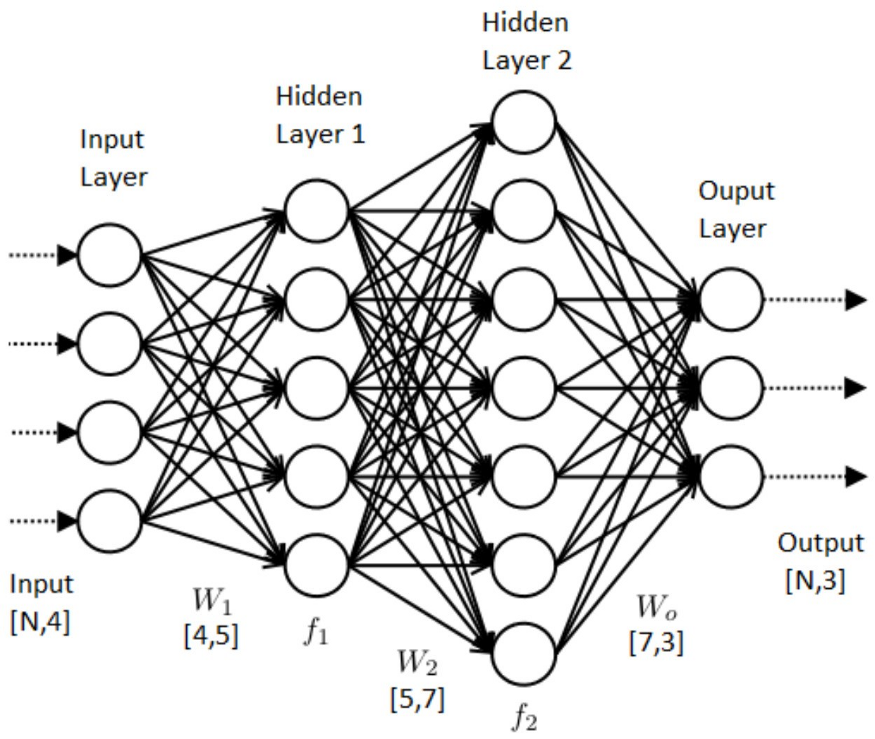
\includegraphics[width=\textwidth/2]{neural_network.png}
\label{neuronovasit}
\caption{Obrázek neuronové sítě. $N$ značí vstupní a výstupní neurony, $W$ značí váhy spojů mezi neurony a $f$ jsou \uv{výpočetní} neurony. Převzato z \url{https://medium.com/coinmonks/the-artificial-neural-networks-handbook-part-1-f9ceb0e376b4}}
\end{figure}

 Využívá se k řešení problémů, které nebylo možné dříve vyřešit (například klasifikace obrázků, rozpoznání slov z lidské řeči a podobně). Neustále se nachází nová využití pro tuto metodu (od překládání jazyků v reálném čase po řízení automobilů).
V oblasti analýzy sentimentu je tato metoda také přelomová. Za správných podmínek dosahuje nejvyšší přesnosti ze všech algoritmů, je však doménově závislá a náročná na trénování.


Koncept je poměrně starý, počátky již v padesátých letech minulého století. Trénování neuronových sítí je výpočetně velice náročné a potřebují velké množství tréningových dat, proto je rozvoj možný až nyní díky výkonnější výpočetní technice (převážně grafickým kartám) a přístupu k obrovskému množství dat. 

Jako spousta dalších algoritmů (hejno částic, mravenčí kolonie a například genetický algoritmus) je i tento inspirován přírodou.
Hluboké učení se snaží napodobit funkci biologického mozku. Neuronová síť je složena z množství neuronů a spoji mezi nimi viz. obrázek~\ref{neuronovasit}. 
Jako v biologickém mozku, každý neuron je schopný zpracovat signál a poslat ho pomocí spojů (synapsí) dalším neuronům. Neuron je v tomto případě vlastně jen obyčejná sčítačka. Všechny vstupy do neuronu jsou vynásobeny váhou daného spoje a sečteny. K~tomuto výsledku se obvykle ještě přičte práh. Po přičtení prahu je použita aktivační funkce (například \emph{sigmoid}, \emph{tanh} nebo \emph{ReLu}) a výsledek je výstupními spoji poslán dalším neuronům. 
Hodnoty prahů a vah spojů jsou z počátku nastaveny náhodně a v průběhu trénování se upravují. 


Hluboké učení je využití neuronových sítí v několikavrstvé architektuře. Architekturu je samozřejmě možné zapojit více způsoby. Pro analýzu sentimentu se nejvíce používají následující architektury neuronových sítí:

\begin{itemize}
    \item Rekurentní - Třída neuronových sítí, kde jednotlivá propojení mezi neurony tvoří cyklus. Každý cyklus je tvořen jednou vrstvou neuronů. Oproti klasické dopředné neuronové síti má vnitřní paměť. Je tedy vhodná ke zpracování sekvenčních dat (mimo jiné i textu). V paměti je uložen aktuální stav zpracování, tento stav je upravován každým příchozím slovem. Stav má tedy uchováno vše, co se postupně zpracovalo. Tento typ neuronových sítí trpí problémem mizejícího a explodujícího gradientu, toho se snaží vyvarovat úpravy této architektury (obousměrné anglicky \emph{bidirectional} architektury a~\emph{LSTM}). 
    \item \emph{LSTM} (\emph{long short term memory}) - Je speciálním typem rekurentní neuronové sítě, která řeší problém mizejícího gradientu. Oproti rekurentní síti má každý cyklus čtyři vrstvy neuronů, které mezi sebou komunikují. Navíc má dva vnitřní stavy místo jednoho. Jednotlivým vrstvám se říká brány a jsou následující: \uv{zapomínající}, \uv{pamatující}, \uv{vstupní} a \uv{výstupní}. Problém mizejícího gradientu je vyřešen kombinací těchto bran a využitím jednoho vnitřního stavu navíc.
    \item Rekurzivní - Tento typ neuronových sítí se obvykle využívá ke zpracování dat v acyklickém grafu (stromu). Je vlastně generalizací rekurentních neuronových sítí. Neuronová síť postupně prochází stromovou strukturu od listů směrem ke kořenu a vytváří rodičovské uzly kombinací jednotlivých tokenů. 
\end{itemize}

Učení neuronových sítí je možné provádět s učitelem, bez učitele a zpětnovazební. Zpětnovazební učení se při analýze sentimentu nevyužívá, proto se na něj nebudu zaměřovat.  

\textbf{Učení s učitelem} je proces při kterém je model učen hledat k danému vstupu korektní výstup. Model tedy hledá funkci $f$ takovou, která bude mít správný výstup $f(x)$ pro co nejvíce vstupních vzorků $x$. Pokud se hledá konkrétní třída z předem dané množiny hovoříme o klasifikaci, pokud se hledá hodnota v určitém rozsahu mluvíme o regresi. Korektní výstupy jsou předem definovány lidmi. Je potřeba mít dostatečně velký počet trénovacích dat, které obsahují vstup a k němu hledaný výstup. Toto může být problematické, protože vytvoření takto označených dat není jednoduché, někdy nemožné. 

V případě analýzy sentimentu bude vstupem text a výstupem hledaný sentiment (pozitivní nebo negativní, popřípadě třídy hodnot). Takto označená data se předají modelu, který se na základě textu pokusí předpovědět výstup (na začátku procesu trénování pravděpodobně chybně). Předpověď je poté porovnána se správnou odpovědí. Porovnání je prováděno tak zvanými ztrátovými funkcemi. Ztrátových funkci je několik, každá se používá pro řešení jiného problému.


Podle chybovosti se modelu upraví proměnné (váhy spojů a hodnoty prahů), aby byl příště přesnější (využívá se derivací pro zjištění správné úpravy). Po dostatečně dlouhém trénování se model naučí potřebné generalizace k tomu, aby byl schopný předpovídat korektně výstup i na datech, které ještě před tím nikdy neviděl.
 
\textbf{Učení bez učitele} využívá pro trénování pouze vstupy \cite{machinelearning}. Hledaný výstup není označen. Analyzátor se snaží ve vstupních datech nalézt strukturu dat a vztahy mezi jednotlivými příklady. Výstupem bývají shluky, kolem kterých se data pohybují. Všechna přiložená data při tréningu se tak strukturují a je možné v nich nalézt podobnosti. 

Podle \cite{unsupervised} je možné pro analýzu sentimentu využít učení bez učitele následujícím způsobem. Využívá se faktu, že negativní nebo pozitivní slova bývají vždy obklopena podobnými slovy. Například slovo \uv{dobrý} je vždy obklopeno obdobnými slovy jako slovo \uv{úžasný}. Tímto způsobem se vytvoří shluk pozitivních a shluk negativních slov. Podle vzdálenosti od středu daného shluku je možné zjisti jak moc pozitivní / negativní dané slovo je. Postupně tak můžeme ohodnotit pozitivitu celého textu.



\section{Pokročilé metody zpracování přirozeného jazyka}
Tato kapitola nabízí přehled novějších technik, technologií a systémů. Základní myšlenka konceptu hlubokého učení je spolu s dalšími základními algoritmy strojového učení popsána v kapitole \ref{machinelearning}. Na základním konceptu hlubokého učení staví mnoho dalších technologií, které zde budou popsány. Samozřejmě existují nové techniky, technologie a systémy, které hlubokého učení nevyužívají. Z osobního zájmu (technologie hlubokého učení mi přijdou zajímavé) se ale soustředím právě na ně. Základní přehled existujících technologií byl nalezen v \cite{survey}.


\subsection{Vnoření slov}
Anglicky známé jako \emph{word embedding}. Vnoření slov je technika jazykového modelování a~reprezentace příznaků. Slova ze slovníku jsou převedena na vektor desetinných čísel. Tento vektor je obvykle vytvořen převedením z řídkého vektoru 1 z $N$ (anglicky \emph{one-hot vector}). Převedený vektor již není řídký, obsahuje nenulové hodnoty ve všech dimenzích (pokud tedy určitá hodnota v dimenzi není reprezentována právě nulou). Zároveň je dimenzí mnohem méně. 

Základní myšlenkou této reprezentace je, že každá dimenze nově vytvořeného vektoru představuje nějakou vlastnost daného slova, podobná slova tedy budou mít podobné číselné reprezentace. Zajímavostí takto vytvořených číselných reprezentací jsou výsledky po matematických operacích mezi slovy. Vlastnost je často vysvětlena následujícím příkladem. Když se vezme vytvořená vektorová reprezentace pro slovo \uv{král}, odečte se od ní vektor slova \uv{muž} a přičte vektor slova \uv{žena}, výsledkem by měla být vektorová reprezentace podobná slovu \uv{královna}.


Vnoření slov je možné využitím hlubokého učení implementovat například metodami \emph{CBOW} \cite{cbow} (\emph{continuous bag of words}), SG \cite{sg} (\emph{Skip-Gram}) a GloVe (\emph{Global Vector}). Metody \emph{CBOW} a \emph{SG} jsou dnes implementovány pod populárním systémem zvaným \emph{Word2Vec}. Tento systém využívá vlastností obou metod pro co nejlepší výsledky. Metoda \emph{CBOW} je přesnější pro menší datové sady, naopak \emph{SG} je přesnější trénováním na větších datových sadách.

Obě metody trénují neuronové sítě velice podobným způsobem. Trénovací data není potřeba anotovat. Metoda \emph{CBOW} učí neuronovou síť předpovědět slovo podle jeho kontextu (kontext je vstupem a slovo výstupem). Naopak metoda \emph{SG} předpovídá kontext podle daného slova (slovo je vstup, kontext výstup). Jeden trénovací příklad by tedy mohl vypadat dle obrázku \ref{trainexample}.

\begin{figure}[!htb]
\centering
\label{trainexample}
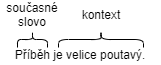
\includegraphics[width=\textwidth/4]{cbow_sg_example.png}
\caption{Ukázka trénovacího příkladu.}
\end{figure}




\subsection{Mechanismus pozornosti pro neuronové sítě}
Tato technika pomáhá řešit problém se vzdálenými závislostmi v sekvenci dat (například závislost mezi prvním a posledním slovem ve větě). Tento problém se snaží řešit oboustranné rekurentní neuronové sítě a LSTM sítě, v praxi je to však stále problematické. 

Tento mechanismus je inspirován vizuální pozorností lidí. Stejně jako lidský zrak se tato metoda soustředí na určitou část ve vysokém rozlišení a okolí je v nízkém rozlišení. Část pod vysokým rozlišením se postupně posouvá v čase. Mechanismus pomáhá trénovanému modelu naučit se které části dat věnovat pozornost na základě vstupu a současného stavu zpracování dat. 


Mechanismus byl například využit v systému pro překlad mezi jazyky \cite{Bahdanau2015NeuralMT}. Pozornost byla využita pro výběr slov relevantních při překladu. Model se postupně soustředí na jednotlivé části překládané věty. Samozřejmě nestačí jít slovo po slovu, protože jazyky často vyjadřují stejnou věc jiným počtem slov. Model se tedy musí naučit toto mapování. Například při překladu z angličtiny do francouzštiny se slovo \emph{destruction} překládá jako \emph{la destruction}, to znamená, že při překladu jednoho slova v angličtině se musí soustředit na vytvoření dvou slov ve francouzštině. 

\subsection{Paměťová síť}


%https://arxiv.org/abs/1410.3916
Anglicky známé jako \emph{memory networks}. V této práci \cite{Weston2015MemoryN} byla síť představena jako systém schopný přijímat logická tvrzení a podle nich poté odpovídat na otázky. Systém je složen z~několika komponent. Jednou z těchto komponent je paměťová část. Paměťová část je oproti například rekurentním neuronovým sítím mnohem větší a dlouhodobější. Jednotlivé části mohou být implementovány jako neuronové sítě, v práci byly prozkoumány i další metody. Paměťová část se chová jako dynamické úložiště znalostí získaných z jednotlivých tvrzení. 
Ostatní komponenty jsou následující:
\begin{itemize}
    \item I (\emph{input feature map}) - převede příchozí data do vnitřní reprezentace
    \item G (\emph{generalization}) - zpracovává příchozí informace (tvrzení), upravuje podle nich paměť znalostí. Má schopnost zestručnit a zobecnit všechny získané znalosti. 
    \item O (\emph{output feature map}) - z již získaných znalostí a nového vstupu vytváří nový výstup. Výstup je stále ve formátu vnitřní reprezentace.
    \item R (\emph{response}) - převádí výstup z vnitřní reprezentace do požadovaného formátu, například text nebo akce.
\end{itemize}

Síť nejprve dostane několik vět a poté otázku, na kterou má odpovědět. Systém je schopný nalézt ve větách potřebné informace a podle nich vytvořit odpověď. Komponenta I přečte jednotlivé věty a přeloží je do vnitřní reprezentace sítě. Poté komponenta G upraví paměť podle nově získaných informací. Po zpracování všech vstupních vět jsou věty uloženy do matice vět. Otázka je také nejprve převedena do vnitřní reprezentace, poté komponenta O nalezne potřebné informace ve vnitřní paměti a vytvoří odpověď. Nakonec je odpověď převedena komponentou R.


\subsection{BERT}

Je zkratka z anglického \emph{\textbf{B}idirectional \textbf{E}ncoder \textbf{R}epresentations from \textbf{T}ransformers}, byl vytvořen společností Google pro lepší pochopení uživatelských vyhledávání \cite{bert}. Tento systém má za cíl naučit se modelovat (dá se říci \uv{pochopit}) jazyk. Technická inovace spočívá ve využití oboustranného trénování transformerů (z anglického \emph{transformer}), což jsou modely využívající koncept pozornosti. Předchozí systémy se obvykle na text dívaly jako na sekvenci slov jdoucí zleva doprava, popřípadě v kombinaci s pohledem zprava doleva. Výsledky systému \emph{BERT} však ukazují, že modely trénované oboustranně mají hlubší pochopení kontextu a sekvencí slov. Vstupní sekvence slov se čte jako celek, to napomáhá modelu se naučit kontext určitého slova na obou stranách. Trénování modelu probíhá následujícími metodami:
\begin{itemize}
    \item maskováním slov - Před předáním trénovací sekvence slov modelu se nahradí 15 \% slov maskovacím tokenem. Model se poté učí předpovědět maskovaná slova podle ostatních slov v sekvenci. 
    \item předpovídáním následující věty - Model postupně dostává dvojice vět. Polovina dvojic vět na sebe navazuje, druhá polovina ne. Model se učí předpovídat jestli druhá věta patří za první či nikoliv. 
\end{itemize}

Model dále využívá toho, že je předem natrénovaný na obrovské sadě dat. Při vytváření modelu pro nový úkol se obvykle musí natrénovat od úplného počátku, to může trvat i~desítky hodin. Tento problém řeší právě předem natrénovaný \emph{BERT}, který pro specifický úkol stačí doladit \cite{finetune}. Autoři systému doporučují dolaďování dvěma až čtyřmi epochami, \emph{BERT} byl v porovnání trénován stovky hodin.    

\emph{BERT} se dnes využívá na množství úkolů zpracování přirozeného jazyka, ve velkém počtu z nich má nejlepší výsledky. Například na těchto stránkách\footnote{\url{http://nlpprogress.com/english/sentiment_analysis.html}} lze vidět všechny jeho využití.


\section{Získání dat z webových portálů}
\label{stahovani}
Před samotným získáním dat je dobré vědět kolik a jakých dat bude potřeba. Proto je vhodné nejprve prozkoumat metody analýzy. Z porovnání metod \cite{approaches} je patrné, že největší přesnost mají analyzátory využívající strojové učení. Z tohoto důvodu bych se přikláněl k~využití těchto analyzátorů. Jejich nevýhodou je nutnost trénování.

Jak je napsáno na tomto blogu \cite{dataamount}, při vytváření analyzátoru na bázi umělé inteligence/strojového učení je potřeba obrovské množství dat pro jeho trénování. O trénování a analýze jsem již psal, nyní stačí informace, že budou potřeba data pro trénování analyzátoru. Těchto dat by mělo být co nejvíce, protože čím větší vzorek dat je použit, tím více vzorů vyjadřování se analyzátor naučí a poté je při samotné analýze přesnější.

Dalším důvodem, proč je potřeba velké množství dat je mimo trénování samotná analýza. Z velkého počtu názorů je patrnější celkový názor na produkt a je pravděpodobnější získat více pohledů na věc.

Z předchozí analýzy tedy vyplynulo, že bude potřeba co nejvíce dat, tato data je možné získat z internetových stránek. Na internetu je velké množství uživatelů a všichni nějakým způsobem přispívají k jeho obsahu \cite{useramount}. Konkrétní počet uživatelů na internetu pro rok 2019 je 4,4 miliard, takové množství uživatelů je schopné vyprodukovat obrovské množství dat každou minutu, konkrétní čísla pro největší sociální média jsou na citovaném blogu.

Uživatelé přispívají na sociálních médiích, speciálních stránkách určených pro recenze nebo přímo na stránkách prodejců. Díky tomu je vytvářeno obrovské množství nestrukturovaných dat, které je možné využít pro analýzu názorů na téměř jakékoliv téma.

Mimo kvantitu dat je také důležitá jejich kvalita. Pokud je analyzátor trénován na špatných datech, nedá se předpokládat, že by měl velkou přesnost. Zpracování dat pro zvýšení jejich kvality je popsáno v kapitole \ref{predzpracovani}. Data (obzvlášť ta stažená z internetových diskuzí) nejsou vždy validní. V případě filmové recenze může být napsána člověkem, který prostě nemá daný žánr rád, nebo může jít o \emph{internetového trolla} \cite{televize}. Ve zkratce, internetový troll je někdo, kdo se snaží narušit věcnou konverzaci nad tématem. Obvykle se snaží z~ostatních uživatelů dostat emocionální reakci.
Validita příspěvku se však nedá jednoduše poznat, proto se musí předpokládat, že každý příspěvek je svým způsobem validní (každý má svůj názor, který se musí vzít v potaz). Při výsledné analýze nevalidní příspěvky příliš nevadí (s nimi se obvykle počítá). Všechny názory jsou důležité, protože utváří celkový pohled na daný film. Pro společnosti je vhodné sledovat všechny názory, aby věděli jakým směrem se dále ubírat, nevalidní příspěvky však při trénování analyzátoru mohou zhoršit jeho přesnost. Validita příspěvků se na některých webech dá poznat pomocí hodnocení (\uv{lajků}) od ostatních uživatelů (tato možnost však není vždy).  

Pro získání dat z webových stránek je hned několik možností. Některé webové stránky mají své rozhraní pro programování aplikací (z anglického application programming interface, zkratka API), pomocí kterého lze požadovaná data získat. Jak píše \cite{webscraping}, API je část serveru odpovědná za přijímání a odesílání požadavků a dat. K tomu jsou obvykle využívány metody GET nebo POST. 

Data jsou odeslána v předem domluveném formátu jako například JSON. Na rozdíl od klasického webového serveru tedy neodesílá HTML dokument, ale pouze požadovaná data.
Při práci s API většinou stačí využít jeho konkrétní knihovnu nebo url adresu a jejich předdefinované funkce. Každá taková funkce má svou dokumentaci, je tedy jasné co funkce vyžaduje a co vrátí. Vše bývá již připraveno pro pohodlí uživatele, je tedy jednoduché se v datech zorientovat, poté je zpracovat a například uložit. Většina stránek však žádné API nemá, nebo k němu dávají přístup pouze ve speciálních případech na zažádání (k přístupu bývá potřeba speciální klíč).
Musí se tedy využít jiné nástroje. 

Obecně se získávání dat z webu mimo použití API říká \emph{web scraping} \cite{webscraping}. \emph{Web scraping} je soubor technik, které lze využít k získání požadovaných (obvykle nestrukturovaných) dat z webových stránek. Mezi tyto techniky patří způsoby pro nalezení hledaných dat i jejich samotné stažení a následné formátování. \emph{Web scraping} zahrnuje široký rozsah programovacích technologií mezi které patří například analýza dat, zpracování přirozeného jazyka a~zabezpečení informací.

Když se provádí automatizovaný \emph{web scraping}, webové stránky můžou být děleny do dvou typů. Stránky používající JavaScript pro vytváření (obvykle dostahování) obsahu, a~stránky bez něj. Při manuálním kopírování dat ze stránky přítomnost JavaScriptu proces neovlivňuje.

Stránky bez JavaScriptu jsou po přijetí požadavku serverem celé odeslány v těle HTTP odpovědi serveru jako HTML dokument. Proto pouze stačí poslat na server HTTP dotaz a~přijatý HTML dokument zpracovat podle potřeby. 

Stránky používající JavaScript pro doplnění obsahu fungují jinak. Nemusí vždy přímo obsahovat hledaná data. HTML dokument obsahuje základní kostru stránky a část dat. Zbylá data jsou načítána dynamicky pomocí skriptů, které se spouští až v prohlížeči uživatele.
Podle toho, jaká data uživatel potřebuje (na co klikl, jestli je přihlášený apod.) JavaScript zašle další požadavky na server. Této technologii se říká AJAX (zkratka z anglického asynchronous JavaScript and XML, neboli asynchroní JavaScript a XML).
Od serveru se vrátí potřebná data obvykle ve formátu JSON a stránka se z těchto částí dat seskládá až v prohlížeči. Proto není možné na server zaslat HTTP požadavek a obdržet zpět stejný HTML dokument jako ten vykreslovaný v prohlížeči.
Pro stahování z JavaScriptových stránek je možné využít \emph{Reverse Engineering} JavaScriptu nebo jeho \emph{Rendering}. \emph{Reverse Engineering} se dělá za pomoci sledování požadavků JavaScriptu a následného zaslání stejných požadavků. Přijatá data se následně seskládají do celku. Druhá metoda je vykreslení a zpracování požadované stránky za pomocí nástroje jako je Selenium. Tento nástroj využívá prohlížeč pro vykreslení stránky a vlastně simuluje návštěvu stránky uživatelem. Po vykreslení webové stránky stačí seskládaný HTML dokument zpracovat podle potřeby.

Jak je napsáno na \cite{shieldsquare} a \cite{jetruby} mezi konkrétní způsoby extrakce dat patří jejich manuální kopírování , \emph{HTML parsing}, \emph{DOM parsing}, využití \emph{XPath}, \emph{google sheets}, a \emph{text pattern matching}. 

Jednotlivé techniky stahování a extrakce hledaných dat jsou popsány v následujících podkapitolách.

\subsection{Manuální kopírování dat}
Anglicky se této technice říká \emph{copy-pasting}. Technika spočívá v prostém kopírování chtěných dat ze zdroje a jejich vkládáním do datového úložiště. Při větším objemu dat tato technika zabere mnoho času a úsilí, práce je velice repetitivní. Na druhou stranu je tato metoda jedinou použitelnou pokud je webová stránka pod ochranou proti stahovacím skriptům. Efektivní je také při získávání pouze malého množství dat. Vzhledem k tomu, jak je tato technika pomalá a neefektivní se moc nevyužívá. Všechny ostatní metody popsané níže jsou automatizované.

\subsection{\emph{HTML parsing}}
Obvykle se dělá za pomocí knihoven jako je například BeautifulSoup. Metoda spočívá ve stažení celého HTML dokumentu a jeho následném prohledání. Využívá se \emph{tagů} a stromové struktury HTML dokumentu. Před napsáním skriptu, který extrahuje hledaná data je nutnost znát stromovou strukturu HTML dokumentu i názvy klíčových uzlů stromu. Strom se poté postupně prochází a extrahují se hledaná data. Cílí na HTML stránky, lineární i~zanořené. Tato metoda je velice rychlá a jednoduchá. Využívá se pro extrakci textu, odkazů zdrojů (např. obrázků) a podobně.

\subsection{\emph{DOM parsing}}
\emph{Document object model} zkráceně DOM, definuje styl, strukturu, ale také obsah dokumentu. Tato technika je schopná získat podrobný pohled na strukturu stránky. Skripty mohou nalézt uzly dokumentu, které obsahují potřebná data a poté pomocí nástroje jako je XPath je extrahovat. Metoda funguje na podobném principu jako \emph{HTML parsing}, místo HTML dokumentu však zpracovává DOM. DOM je oproti HTML dokumentu dynamický, takže tahle metoda je použitelná i když stránka obsahuje části generované dynamicky.

\subsection{\emph{google sheets}}
Jednou netradičnější, ale přesto efektivní metodou je využití google tabulek. Tabulky mají funkci s názvem \emph{IMPORTXML}, které stačí předložit odkaz na danou stránku. Pokud stránka není chráněna, funkce vrátí XML strukturu této stránky i s jejím obsahem.

\subsection{\emph{text pattern matching}}
Využívá regulárních výrazů k extrakci hledaných dat (například UNIXový grep). Klasicky se tato metoda pojí s nějakým skriptovacím jazykem jako je Python nebo Perl. Regulární výraz je speciální textový řetězec, který pomocí předdefinovaných značek určí hledaný vzor textu.


Mimo tyto metody existují další dostupné nástroje pro extrakci dat jako je například cURL, Wget, HTTrack, Node.js a další.


\section{Možnosti uchování získaných dat}
\label{ukladani}
Data je možné ukládat v jejich nestrukturované (původní) formě, nebo se z nich extrahují pouze potřebné části. Od tohoto se bude odvíjet i způsob uložení daných dat. Pokud data nemají žádnou strukturu, ukládání do serializované podoby nebo databáze by pouze přidalo režii a nijak by to na rozdíl od prostého uložení do souboru nepomohlo.
Na druhou stranu, po zpracování dat do strukturované podoby, je vhodné využít serializačních formátů nebo databáze. Takový způsob uložení napomůže v pozdějším vyhledávání a analýze těchto dat.

Zde bych se chtěl věnovat různým možnostem ukládání stažených dat. Nejčastěji stahovaná a ukládaná data budou textového typu, proto bych chtěl rozebrat právě možnosti ukládání textu (využitelné však i pro jiná data).
Pro ukládání textových dat jsou v podstatě dvě možnosti. Data uložit přímo do textového souboru nebo využít nějakého databázového systému. Detaily v podkapitolách.


\subsection{Uložení do souboru}
Do souboru je možnost ukládat data ve zdrojové podobě (například ukládání celých HTML dokumentů zdrojových stránek). Data můžou zůstat v originálním formátu pro pozdější zpracování, nebo jsou nějakým způsobem předzpracovány (odstranění HTML značek a ponechání čistého textu) a poté uloženy. Tato metoda je však většinou nepraktická, protože se v takovýchto datech nedá jednoduše vyhledávat a data nejsou tak přehledná.

Pro ukládání do souboru se proto obvykle využije serializace. 
Serializace je proces převádění strukturovaných dat do formátu, který umožňuje uložení nebo přenos těchto dat a~jejich následné znovupoužití. Serializovaná data mohou být v souboru uložena v textové podobě (čitelné i pro člověka) nebo v binární podobě (bez deserializace čitelné pouze pro počítač). Serializovaná data se ukládají persistentně, to znamená že se data neztratí po ukončení programu nebo například výpadku proudu. Takto uložená data je díky jejich jednotnému formátu možné použít i na jiné počítačové platformě (jiné součástky, jiný operační systém).
V serializovaných datech se vyhledává mnohem lépe než v těch nestrukturovaných díky ukládání částí dat pod názvy atributů. 


Mezi nejpoužívanější serializační formáty patří JSON, XML, YAML, CSV a TSV.


\subsection{Uložení do databáze}
Databáze je organizovaná kolekce dat obecně uložená v elektronické podobě na počítačovém systému (obvykle serveru) \cite{oracle}. 
Implementačně je databáze vlastně kolekce souborů, do kterých se ukládají data. Rozdíl oproti klasickému uložení do souboru je takový, že zde se o~tyto soubory stará systém řízení báze dat (SŘBD). SŘBD slouží jako rozhraní mezi databází (kolekcí souborů) a jejími koncovými uživateli nebo programy, které s databází komunikují. SŘBD Umožňuje uživateli pohodlnou práci s daty. Dále je díky tomuto systému možné určovat jakým způsobem budou data organizována a optimalizována (například indexací). SŘBD napomáhá se správou databáze sledováním transakcí v databázi, monitorováním výkonu, zálohou a obnovením databáze. Tento systém dále umožňuje autentizaci a autorizaci pro ochranu uložených dat. Databáze může být vytvořena lokálně nebo na serveru, se kterým se komunikuje přes internet.

Typů databází je několik, nejběžněji se používá relační a objektová. Data jsou v relační databázi organizována jako série tabulek, kde řádky tabulky jsou jednotlivé záznamy (například záznam o osobě) a sloupce tabulky jsou jednotlivé atributy sledované u tohoto záznamu (jméno, věk a pohlaví osoby). Toto umožňuje jednoduše vyhledávat, upravovat nebo přidávat data. Mimo tyto jednoduché akce existují takzvané agregační funkce (například dotaz na průměrný věk osoby). 
Databáze nejsou stěžejním tématem této práce, proto jsem popsal pouze úplné základy. Databází je mnohem více typů a používají různé jazyky (SQL, NOSQL apod.), ale dále to tu nechci rozvádět.


\section{Předzpracování textu pro následnou analýzu}
\label{predzpracovani}
Předzpracování textu (anglicky preprocessing) je množina kroků, které se provádí s daty před tím, než jsou analyzována.

Při použití analyzátoru založeném na hlubokém učení je povinný pouze krok převedení textu do číselné podoby. Důvod je takový, že tyto modely jsou schopny pracovat pouze s~čísly \cite{mlexplained}. Konkrétní metody převedení textu na číselnou reprezentaci budou popsány dále. Většina ostatních metod převod na číselnou podobu nepotřebuje. 

Další kroky předzpracování nejsou pro funkčnost analyzátorů klíčové, avšak tyto kroky napomůžou s přesností analýzy (přesností je zde myšlen poměr mezi počtem správných předpovědí analyzátoru a celkovým počtem předpovědí). 

Dalším z cílů předzpracování textu je převést vstupní text do predikovatelné, analyzovatelné podoby a odstranit šum. Šumem se v tomto kontextu myslí všechen nesmyslný text nebo znaky. Šum je pro analýzu irelevantní popřípadě škodlivý. Pokud se do analyzátoru vloží nekvalitní data, nedají se očekávat kvalitní výsledky. 
Odstraněním šumu a normalizací slov dosáhneme dvou cílů. 

Za prvé, analyzátory mají obvykle limitovanou velikost slovníku. Odstraněním irelevantních slov nebo znaků a sloučením více tvarů slova do jednoho necháme ve slovníku prostor pro užitečnější slova.
Za druhé, při výsledné analýze (analyzovaný text se také předzpracuje) bude analyzátor považovat různé tvary jednoho slova za stejné. Nestane se tedy, že by ve slovníku měl slovo \uv{dobrý} a slovo \uv{dobry} by nerozpoznal.

Předzpracování textu tedy může být rozděleno na normalizaci (úpravu textu do normální formy), tokenizaci (rozdělení textu na atomické části, těmi může být slovo nebo věta) a převedení do číselné podoby. Text převedený do číselné podoby je již možné použít v~analyzátoru založeném na hlubokém učení.

\subsection{Normalizace}
Normalizací je v kontextu NLP myšleno převedení textu do normální (kanonické) formy~\cite{mlexplained}. Cílem tohoto kroku je z textu odstranit všechny nechtěné znaky a slova převést do správné formy. Text je převeden do čisté formy odstraněním všech nepotřebných řetězců a~znaků. Tento krok je velice důležitý obzvlášť pokud je použit text z internetových diskuzí. Tento text je velice často psán nespisovně, obsahuje různé speciální znaky, gramatické chyby a~slangové výrazy. Normalizací se všechna tato slova převádí do jednoho (obvykle jejich spisovného) tvaru. Důvodem je to, že po převedení slov do číselné reprezentace by se slova \uv{film},\uv{fiilm} a \uv{Film} brala jako  úplně odlišná. Zvláštní nepotřebné znaky se obvykle úplně odstraňují. Odstraňování je prováděno například regulárními výrazy.

Při normalizaci se musí dbát na to, co je cílem následné analýzy. Pokud cílem analýzy by bylo předpovědět emoce autora textu, bylo by velice nevhodné převádět všechna písmena na malá a odstranit speciální znaky, ze kterých mohou být seskládány emotikony. Velikost písmen a emotikony totiž nesou emocionální informaci, kterou je vhodné zpracovat. 
Tímto se snažím naznačit, že je potřeba určit správnou úroveň normalizace a odstraňovat pouze to, co není užitečné. Na \cite{mlexplained} se dá zjistit, kolik normalizace je potřeba v jaké situaci. Čím více je trénovacích dat, tím méně normalizace je potřeba, protože model je schopný se z~nich naučit všechny potřebné detaily (že např. slova film a Film jsou vlastně totožná). Dále se také musí myslet na to, jak šumivý daný text je, popřípadě jaký je jeho obsah. Čím šumivější text je, tím je normalizace více potřeba. Pokud obsah textu není dostatečně obecný (všechna data si jsou dosti podobná) je lepší použít více normalizace.

Nejjednodušším, ale přesto efektivním způsobem normalizace textu pro analýzu sentimentu je \textbf{převedení všech písmen na malá}. Tímto se předejde problému v předchozím příkladě s malým nebo velkým písmenem na začátku slova (\uv{film} vs. \uv{Film}) a odstraní se redundantnost ve slovníku. Pokud je tento způsob normalizace použit při tréningu, musí se poté použít i při samotné analýze dat. Analyzátor by všechna slova s velkým písmenem neměl ve slovníku (neznal by je) a snížila by se přesnost.
Při analýze sentimentu velikost písmen nehraje roli. Spíše při ní jde o celkové vyznění dané recenze, proto je vhodné tento způsob normalizace využít.

Po již popsaném odstranění nechtěných znaků, převedení slov do gramaticky správné formy (například \uv{supeeer} na \uv{super}) a jejich úpravy na pouze malá písmena, můžeme text upravovat dále. Mezi takové úpravy patří odstranění stop slov, lemmatizace a stematizace.


\textbf{Odstranění stop slov} je proces při kterém se odstraňují všechna slova s velice malou informační hodnotou pro analýzu. Opět záleží na cíli analýzy, ale obvykle tato slova jsou zájmena, předložky a spojky. Často se odstraňují i čísla, většinou nenesou velkou informační hodnotu. Myšlenkou je odstranit všechny nedůležitá slova a soustředit se na ta důležitá, tato metoda však při použití hlubokého učení přesnost příliš nezvýší.



\textbf{Stematizace} a \textbf{Lemmatizace} jsou velice podobné metody. Obě se snaží najít kořenový tvar všech slov v textu. Cílem je opět snížit počet slov ve slovníku, protože se z několika slov stane jedno (například z \uv{natáčejí a \uv{natočil} se stane \uv{točit}}. Lemmatizace se snaží nalézt opravdový spisovný kořen slova. Oproti tomu stematizace používá heuristik pro vytvoření nějakého kořenu, který často ani není opravdovým slovem.




\subsection{Tokenizace}
Jak už název napovídá, cílem tohoto kroku je rozdělit analyzovaný text na tokeny. Tokenem může být jakákoliv pro analýzu významná část textu (slovo, věta, odstavec) \cite{gdcoder}. Podle způsobu tokenizace jsou při procesu odstraňovány oddělující znaky (mezery, tečky, čárky a~podobně). 
Podle \cite{mlexplained} je tokenizace velice komplexní a důležitý krok předzpracování textu, přesto mu není věnována dostatečná pozornost. Přestože se tento krok zdá triviální, jeho správné provedení je důležité pro zvýšení přesnosti a odstranění chyb v systému.

Určení správného způsobu rozdělení textu je závislé na cíli tohoto kroku a jazyku (popřípadě typu textu) na kterém je tokenizace prováděna. 

Pro analýzu sentimentu se obvykle rozděluje text na věty nebo slova.
Při tokenizaci textu na slova máme několik možností.
První z nich jsou \textbf{naivní tokenizační algoritmy}, které slepě rozdělují text podle mezer. Nastává problém s interpunkcí ve větě. Interpunkční znaménka se \uv{přilepí} k nějakému slovu, tím vznikne slovo, které analyzátor nezná a vznikne přesně ten problém, který je předzpracováním snaha odstranit. 


O něco lepším přístupem je oddělovat slova podle mezer a interpunkčních znamének. Tímto se odstraní předchozí problém, ale vzniknou další. Algoritmus selhává například se zkratkami (\uv{U.S.A}) nebo u slov obsahující uvozovky a apostrofy. Dalším problémem jsou různé speciální znaky, které by mohly být pro určité typy analýzy potřebné (např. emotikony a odkazy).

Kvůli těmto a dalším problémům je nutné využít komplexnější \textbf{tokenizátory založené na pravidlech}. Možnost mít pro každý případ pravidlo, jak se má s textem nakládat pomáhá řešit všechny předem zmíněné problémy. Tato metoda se dá implementovat například regulárními výrazy, ale není to příliš doporučováno. Při komplexnějších pravidlech se začnou objevovat chyby, které se těžko opravují. Lepším přístupem je využít již existující implementace jako jsou například Spacy, Moses nebo NLTK tokenizátor. Implementace mají již předem vytvořená pravidla pro nejčastější případy v různých jazycích. Nejprve vše rozdělí klasicky podle mezer a poté projdou jednotlivé tokeny a pročistí je. Oddělí se interpunkce a podobně. Uživatel těchto knihoven si samozřejmě může specifikovat svá vlastní pravidla, kdy tokenizovat a kdy ne. Implementované knihovny jsou schopny provádět jak tokenizaci na slova tak na věty.


Speciálním případem tokenizátoru, který se snaží ještě dále zlepšit přesnost systému je \textbf{\uv{subword tokenizer}}. Název napovídá jeho funkci. Metoda má mnoho konkrétních implementací, každá využívá trochu jiný algoritmus. Detaily o každém z nich jsou na \cite{mlexplained}. Všechny algoritmy sdílí hlavní myšlenku toho, že všechny často se objevující slova by měly mít svá vlastní id (označení po převedení do číselné reprezentace). Méně častá slova se skládají z jejich částí. Tento způsob pokrývá velké množství slov za využití co nejmenšího počtu id, tedy slov, které si tokenizátor musí uložit do slovníku. Tento tokenizátor se musí natrénovat na datech, aby se naučil nejčastější slova a části těch méně častějších. Je tedy potřeba mít trénovací data. Po natrénování tokenizátoru jsou využita naučená slova, popřípadě části slov k rozdělení analyzovaného textu. 



\subsection{Převedení textu do číselné podoby}
Jak již bylo řečeno dříve, analyzátory založené na hlubokém učení nepracují přímo s textem, ale s čísly. Z tohoto důvodu se vstupní text (ať už při tréningu nebo při samotné analýze) musí převést na číselnou reprezentaci.

Nejjednodušším způsobem, jak převést slova na čísla by samozřejmě bylo vzít seznam všech nalezených slov a každému z nich přiřadit nějaké číslo \cite{wordtonumber}. Takže z věty \uv{Film se mi líbil.} by byl vytvořen slovník, kde slovo \uv{Film} by bylo reprezentováno číslem 1, slovo \uv{se} číslem 2 a podobně. 


Tenhle způsob by v určitých situacích byl použitelný, ale musí se počítat s tím, že analyzátor s čísly provádí výpočty. Slovo reprezentované vyšší hodnotu by se chovalo, jako by mělo větší váhu, takové chování není vždy chtěné.

Řešením je převést danou číselnou hodnotu na kód $1$ z $N$. Tento kód reprezentuje každé slovo (jeho číselnou hodnotu) pomocí vektoru. Vektor má velikost takovou, jak dlouhý je celý slovník (pokud je ve slovníku 10 000 slov, vektor bude mít 10 000 prvků). Ve vektoru se na indexu, který se rovná číselné hodnotě slova přičte jednička, zbytek budou nuly. Pro předchozí příklad by tedy slovo \uv{Film} mělo vektor $[1,0,0,0]$, slovo \uv{se} by mělo vektor $[0,1,0,0]$ a tak dále. Využitím této metody je možné reprezentovat jakkoliv dlouhý text. Této metodě se anglicky říká \emph{bag of words}. Je schopná reprezentovat slova v textu i jejich počet, ale není schopná zachytit jejich kontext, tedy jaká slova se vyskytují kde. Reprezentaci je možné vylepšit využitím n-gramů nebo tf-idf \cite{bow}. 

  \chapter{Návrh systému}
\label{navrh}
Cílem této kapitoly je podívat se na vytvářený systém z abstraktnějšího pohledu a prozkoumat jednotlivé akce, které bude systém provádět. Akcí bude několik, proto systém bude rozdělen do logických celků, které obstarávají určitou část procesu analýzy. Na každou z~těchto částí jsou kladeny určité požadavky, které musí být splněny. 

Systém je navrhován postupně, podle jednotlivých kroků analýzy. Prvním krokem je obstarání dat, druhým je jejich uložení, dále pak jejich zpracování a analýza. Informace získané analýzou poté budou prezentovány. 

\section{Získání dat}
Jak již bylo popsáno v teoretickém rozboru (kapitola \ref{stahovani}), data jsou pro tento systém velice důležitá. Dále bylo rozebráno, že budou potřeba data pro trénování i samotnou analýzu. Trénovací datová sada by měla ideálně obsahovat anotace hledaných odpovědí klasifikátoru. Recenzí bude potřeba co nejvíce a při jejich větším počtu nepřipadá manuální anotace (označování) v úvahu. Z tohoto důvodu by bylo ideální najít zdroj recenzí, kde jsou jednotlivé recenze již anotovány. Možností jejich získání je hned několik, záleží na konkrétním zvoleném zdroji. Nejpohodlnějším způsobem získávání recenzí by bylo za využití \emph{API} dané webové stránky, další možností je využít jednu z popsaných technik extrakce dat v~kapitole~\ref{stahovani}. 

Možných zdrojů dat je velké množství, lidé dnes využívají pro sdíleních svých názorů sociální média, blogy, fóra, specializované stránky pro recenze a další. 

Získávání dat ze sociálních médií je pravděpodobně nejjednodušší, protože obvykle nabízí \emph{API}. Na druhou stranu data na sociálních médiích neobsahují požadované anotace, poměrně často bývají irelevantní a kvůli zvyšujícímu se soukromí na těchto platformách se informace stávají nepřístupnými. 

Dále by se daly využít již vytvořené datové sady. Komunita věnující se zpracování přirozeného jazyka je velice aktivní po celém světě, takže se dá nalézt již anotovaná datová sada téměř v jakémkoli jazyku. Tento přístup by se dal využít k počátečnímu natrénování klasifikátorů, systém by však měl být schopný automaticky a pravidelně stahovat nové recenze, aby zůstal aktuální. 

Nejlepším zdrojem dat tedy nejspíš bude některá z webových stránek specializujících se na filmové recenze. Tyto stránky splňují všechna dříve zmíněná kritéria. Navíc velké platformy obvykle  mají i vlastní \emph{API}, které by zjednodušilo získávání recenzí. 

\subsection{Extrahované informace}
Nezávisle na zdroji recenzí, ze získávaných příspěvků bude pro úspěšnou analýzu nutnost získávat určité informace. Nejdůležitější je samozřejmě samotný text recenze, dále je však potřeba číselné hodnocení autora pro následné porovnání hodnot při trénovaní klasifikátorů. Další důležitou informací je cíl dané recenze (tedy film, kterého se recenze týká). Uživatelské jméno autora se dá využít k případné identifikaci této recenze, popřípadě k přiřazení váhy k~recenzi na základě toho, kdo danou recenzi napsal. Datum vytvoření recenze bude užitečné pro sledování postupné změny názorů v čase. Poslední získávanou informací by měla být webová stránka, ze které byla recenze stažena. Tato informace je důležitá pro následné nalezení recenze a pro identifikaci jazyka recenze (systém by měl pracovat pro český i~anglický jazyk).

\subsection{Ukládání dat}
Zmíněno v teorii (kapitola \ref{ukladani}), k uchování získaných dat je více možností. Tento systém by však nejlépe fungoval s využitím relačního databázového systému. Důvodem je strukturovanost extrahovaných dat (bude stačit ukládání do tabulek, není tedy potřeba NoSQL databáze). Na druhou stranu ukládání do souborů (v serializačním formátu) by nebylo velice moudré, protože je předpokládané velké množství recenzí a k uloženým datům bude pravděpodobně přistupovat více částí systému najednou. Velké soubory se pomalu zpracovávají a není možné s nimi pracovat z několika míst najednou. 

\section{Analýza dat}
Po získání a uložení dat v systému navazuje jejich analýza. Data by měla být ukládána ve své původní formě, tedy neupravené, pro zachování co nejvíce informací. Před samotnou analýzou by se však měla předzpracovat využitím technik popsaných v kapitole \ref{predzpracovani}. Předzpracování pomáhá systému zvýšit jeho přesnost. 

Nejvyšších přesností dosahují metody klasifikace založené na strojovém učení, z tohoto důvodu bude tato část systému rozdělena na část pro trénování klasifikátoru a část využívající natrénovaný klasifikátor. 

Recenze bych analyzoval na úrovni dokumentu a úrovni aspektu. Na úrovni dokumentu by byla prováděna polaritní analýza (pozitivní / negativní polarita), dále pak analýza míry této pozitivity (jedna až pět, nebo jedna až deset hvězd). Dále by mohla být prováděna analýza na úrovni aspektu pro získání detailnějších informací z recenze. Ke zjištění jaké aspekty budou analyzovány bude potřeba prozkoumat uživatelské recenze a zjistit o čem uživatelé nejčastěji píší. Pro aspektovou analýzu bude oproti ostatním nutné ručně anotovat recenze, nalézt již vytvořenou datovou sadu se mi asi nepodaří.

Analýzu je možné provádět množstvím metod, chtěl bych jich tedy vyzkoušet několik a~porovnat jejich výsledky. 

Výsledky analýzy by se měli opět ukládat do relační databáze pro jejich následné zpracování a zobrazení.

\section{Zpracování a vizualizace výsledků}
Pouhý soupis výsledků jednotlivých analýz by toho moc neprozradil. Je tedy vhodné výsledky agregovat a poté je zobrazit například grafem. K tomuto bych využil webové rozhraní z důvodu pohodlí uživatele. Nemusí nic stahovat ani instalovat, může se na stránky podívat téměř na jakémkoliv zařízení a uživatelé by si například mohli vytvořit vlastní účty.

Jednotlivé recenze a jejich výsledky bude samozřejmě nutné seskupit podle filmu, kterého se týkají. Uživatel poté může vyhledávat daný film, nebo procházet žebříček těchto filmů podle výsledných hodnot analýz. Dále by mohly být sledovány různé trendy titulů (popularita žánrů, jestli jsou populárnější filmy či seriály a podobně). 

\section{Výsledný systém}
Jednotlivé části systému by spolu měly komunikovat dle obrázku \ref{schema}.

\begin{figure}[!htb]
\label{schema}
\centering
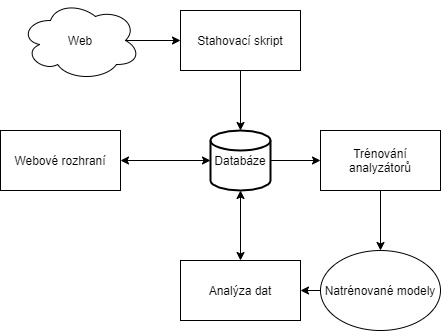
\includegraphics[width=\textwidth/2]{system_diagram.png}
\caption{Architektura navrhovaného systému. Jednotlivé části budou ovládány nástrojem pro plánování úloh.}
\end{figure}


\chapter{Implementace systému}
\label{implementace}
%\todo{INFORMACE VS DATA??, MUZU TAKHLE POUZIVAT?}
%\todo{OPRAVIT SLOVA TRCICI MIMO TEXT}
V této kapitole popisuji implementaci dříve definovaného systému. 
Systém je rozdělen do následujících částí:  

\begin{itemize}
  \item Stahování potřebných dat.
  \item Databáze.
  \item Trénování analyzátorů.
  \item Analýza sentimentu.
  \item Rozhraní pro zobrazení výsledků analýzy.
\end{itemize}

Pro každou z těchto částí je věnována samotná podkapitola. Při popisu každé z částí jsou nejprve prozkoumány možnosti řešení, které byly brány při v potaz a následuje popis výsledné implementace. 

Převážná většina systému je vytvořena v jazyku Python verze 3.6.9. Je využito několik pomocných skriptů pro bash. Výsledky analýzy jsou uživateli zobrazovány v prohlížeči za použití webového aplikačního rámce Django.
Systém běží na školním serveru \emph{Athena1} a je implementován pro češtinu i angličtinu. 

Protože je na systém požadavek pravidelné aktualizace dat, skripty pro stahování, zpracování dat a sémantickou analýzu je možné spouštět manuálně i automaticky. Postupně se tedy zvětšuje počet uložených recenzí v databázi. Tyto recenze jsou poté (opět automaticky) analyzovány natrénovanými klasifikátory. Natrénování klasifikátorů se dělá manuálně.

Automatické spouštění všech skriptů je prováděno pomocí plánovače úloh \emph{Cron}. Úlohy plánovače (takzvané \emph{Cronjobs}) jsou zapisovány do souboru zvaném \emph{Crontab} a mají následující formát:
\begin{center}
minuta[0-59] hodina[0-23] den měsíce[1-31] měsíc[1-12] den týdne[0-6] příkaz ke spuštění
\end{center}
%\todo{Popsat jak přesně funguje cron? musel bych najít na netu}

Namísto konkrétních čísel je možné využít znak hvězdičky, který zastupuje každou instanci (každou minutu, každou hodinu a podobně).
Z toho vyplývá že \emph{Cron} umožňuje spouštění jednou v konkrétní čas, ale i pravidelně.

\emph{Cron} nespouští přímo požadovaný python skript, ale jeden z dříve zmiňovaných bash skriptů. Tento bash skript nejprve zapne vývojové \emph{Conda} prostředí obsahující všechny systémem používané knihovny a potom až daný python skript.

Většina skriptů tvořících tento systém nějakým způsobem pracuje s daty, potřebují tedy přístup k nějakému úložišti dat. 
\clearpage
\pagebreak
Pro ukládání dat jsou podle potřeby využity:
\begin{itemize}
    \item Lokální soubory, formátu JSON nebo prostého textu.
    \item PostgreSQL databáze.
    \item SQLite databáze.
\end{itemize}

 

\section{Stahování dat}
Původně měli být zdroje dat Facebook a Twitter.
To se ovšem ukázalo jako ne tím nejlepším řešením, protože data ze sociálních sítí nebývají příliš kvalitní. Obě platformy mají navíc limitovaný přístup k datům a chybí zde číselné ohodnocení od autora.

Rozhodl jsem se tedy využít weby pro recenze filmů, kde jsou příspěvky relevantnější (uživatelé více vyjadřují svůj názor) a jsou dostupná číselná hodnocení od uživatelů. Díky číselnému hodnocení nemusí být texty recenzí manuálně anotována a hodnocení může být použito jako referenční výsledek pro trénování analyzátorů.
Toto řešení není úplně ideální, protože uživatelé občas dají pozitivní hodnocení (celkově se jim film líbil) a do textu recenze napíší všechny chyby filmu (určité části nebo detaily, které se jim nelíbily). Tohle by mohlo analyzátor při trénování zmást. Ideální by asi bylo data překontrolovat a hodnocení podle obsahu textu změnit. Dat je však tolik, že tohle není možné provést.


Zdroji dat se tedy staly weby \emph{csfd.cz}, \emph{fdb.cz}, \emph{rottentomatoes.com} a \emph{imdb.com}.
Pro získání dat z webových portálů jsem se pokusil získat přístup k jejich API, žádný z webů mi však nevyhověl (portál rottentomatoes.com má pro tento účel dotazník). 
Ke stažení recenzí z~daných webových stránek  tedy byly vytvořeny skripty využívající \emph{web scraping}. Každý portál má svůj vlastní skript. 

Všechny skripty pro stahování recenzí (kromě toho pro čsfd) mají společnou třídu \emph{Database\_manager} v souboru \emph{database\_manager.py}. Tato třída má na starost práci s PostgreSQL databází. Databáze běží na školním serveru \emph{Athena1}. Třída zajišťuje připojení a~přihlášení k databázi a implementuje několik funkcí pro dotazy a ukládání dat.

Stahování dat se spouští třídou \emph{Data\_downloader} v souboru \emph{data\_downloader.py}. Tato třída pouze podle nastavení v souboru \emph{config.py} spouští jeden stahovací skript za druhým.

Detailně jsou jednotlivé způsoby stahování dat popsány v následujících podkapitolách. 


\subsection{Stahování z ČSFD}

Stahování z této webové stránky je implementováno třídou \emph{Web\_scraper\_csfd} v souboru \emph{web\_scraper\_csfd.py}. Webové stránky \emph{csfd.cz} jsou celé implementovány staticky (nevyužívají JavaScript pro doplňování obsahu stránky). Z tohoto důvodu je stahování prováděno za využití knihovny \emph{urllib}, která umožňuje zasílat HTTP požadavky. Tato knihovna je implicitně součástí Python distribuce. Po získání HTTP odpovědi serveru jsou data zpracována pomocí knihovny \emph{BeautifulSoup} verze 4.8.2. Knihovna umožňuje procházet stromovou strukturou HTML dokumentu. 
Pro extrakci hledaných dat je nutné si nejprve projít strukturu stránky. Nejpohodlnější je využít funkci \uv{Prozkoumat}, kterou má každý webový prohlížeč a zjistit kde se ve stromové struktuře data nachází. Podle toho pak stačí využít vyhledávací funkce knihovny \emph{BeautifulSoup}. Možné je vyhledávat například podle názvu HTML značky, jejího id nebo třídy (class). Možností je samozřejmě více, pro detail má knihovna dokumentaci\footnote{\url{https://www.crummy.com/software/BeautifulSoup/bs4/doc/}}.

K vytvoření datové sady pro trénování analyzátorů i následnou analýzu jsou ke každé recenzi získávány následující informace:
\begin{itemize}
    \item Název titulu, ke kterému se recenze vztahuje.
    \item Text recenze.
    \item Hodnocení uživatele, na čsfd může uživatel hodnotit nula (odpad!) až pěti hvězdičkami, hodnota je před uložením normalizována na hodnotu mezi nulou a jedničkou.
    \item Identifikační číslo uživatele.
    \item Datum zveřejnění recenze.
\end{itemize}

Stahování nebylo možné provádět přímo na školním serveru \emph{Athena1}, protože po odeslání požadavku ze školního serveru na webový server se vždy vrátilo chybové hlášení. Z tohoto důvodu byl skript spouštěn na mém osobním počítači. 

K databázi na školním serveru se z venkovní sítě nedá připojit. Z tohoto důvodu byla na osobním počítači použita databáze SQLite. Databáze byla použita pro zaznamenávání již stažených příspěvků, aby skript nestáhl jeden příspěvek několikrát. Tabulka těchto záznamů má dva sloupce. Jeden pro název titulu a jeden pro identifikační číslo autora recenze. Předpokladem je, že každý uživatel napíše maximálně jednu recenzi ke každému titulu. 


Princip algoritmu pro stahování dat je následující. Nejprve se skript připojí k SQLite databázi pomocí třídy \emph{Database\_manager\_csfd}. Poté je zavolána funkce \emph{download\_all}, která započne stahování. Algoritmus využívá postupně vzrůstajícího identifikačního čísla uživatelů. Identifikační číslo uživatele od kterého má skript začít stahovat je nastavováno manuálně pro lepší kontrolu nad skriptem (alternativně by se mohlo číslo nastavit podle posledního záznamu v databázi). 
Postupně se tedy přičítá číslo aktuálního uživatele a prochází se odkazy následujícího formátu:
\begin{center}
    https://www.csfd.cz/uzivatel/<identifikační číslo uživatele>
\end{center}

Přijetím odpovědi serveru se zjistí, jestli účet uživatele s daným identifikačním číslem existuje. Pokud byl účet smazán, vrátí se chybová odpověď. Algoritmus si zaznamenává počet po sobě jdoucích chybových odpovědí. Pokud tato hodnota překročí určitou mez, stahování končí, protože algoritmus došel na konec seznamu identifikačních čísel uživatelů (identifikační čísla ještě nikdo nepoužívá). 

Pokud se od serveru vrátí pozitivní odpověď, přejde se do komentářové sekce uživatele. Postupně se prochází všechny komentáře daného uživatele a stahují se dříve zmiňované informace. Identifikační číslo uživatele a název komentovaného titulu se porovná se záznamy v SQLite databázi. Pokud takový záznam ještě neexistuje, tak se v databázi vytvoří a~informace se uloží. V opačném případě se informace zahodí. 
Stažená data jsou ukládána do lokálního souboru ve formátu JSON a později vložena do databáze na školním serveru. K uložení dat do školní databáze se používá pomocný skript \emph{upload\_csfd.py}. Na školním serveru jsou recenze ukládány do tabulky \emph{reviews}. 



\subsection{Stahování z FDb}
Implementováno třídou \emph{Web\_scraper\_fdb} v souboru \emph{Web\_scraper\_fdb.py}. Stejně jako\linebreak webové stránky čsfd jsou i tyto implementovány plně staticky, využívají se tedy stejné\linebreak nástroje (\emph{urllib} a \emph{BeaurifulSoup}). Stránky samozřejmě mají jinou strukturu než čsfd, proto je nutné je také projít (využitím nástroje \emph{Prozkoumat}) a vyhledat všechny důležité elementy HTML dokumentu. 

Seznam získávaných informací se oproti tomu z čsfd liší pouze v použití uživatelských jmen namísto identifikačních čísel.

Na rozdíl od skriptu pro čsfd, tento byl spouštěn na školním serveru. Byla tedy využita školní PostgreSQL databáze. K připojení a provádění akcí s databází je využita již zmiňovaná třída \emph{Database\_manager}. Pro záznamy již stažených recenzí (aby se jedna recenze nestáhla několikrát) je využita tabulka s názvem \emph{users\_fdb}, která funguje stejným způsobem jako SQLite databáze pro čsfd. Výsledné informace o recenzích jsou přímo ukládány do tabulky \emph{reviews}. 

Algoritmus funguje velice podobným způsobem jako při stahování z čsfd. Hlavním rozdílem je způsob procházení stránky (důvodem je samozřejmě jiná struktura stránek). 

Dalším rozdílem je postupné procházení uživatelů, které v tomto případě nevyužívá identifikačního čísla. Uživatelé i zde identifikační čísla mají a odkazy na uživatelské účty by se daly procházet stejným způsobem jako u čsfd. Stránky však při neexistenci uživatelského účtu s daným identifikačním číslem neodpoví chybovým hlášením. Namísto toho přesměrovávají na hlavní stránku (fdb.cz). Z tohoto důvodu jsou uživatelé nejprve vyhledáni v~žebříčku uživatelů a až poté se stahují jejich příspěvky.



\subsection{Stahování z Rotten Tomatoes}
Provádí třída \emph{Web\_scraper\_rottentomatoes} v souboru \emph{Web\_scraper\_rottentomatoes.py}.

Stránky jsou pouze částečně statické. 
Stahování dynamických stránek je mnohem pomalejší, protože se musí využít prohlížeče pro jejich vykreslení. Z tohoto důvodu jsem se rozhodl stahovat pouze statickou část stránek. Využité knihovny a základní postup procházení stránek je tedy pořád stejný. Stahování dynamických stránek jsem využil až pro stránky imdb, kde je u každého titulu mnohem více recenzí a tak se čekaní na načtení stránek více vyplatí. Například pro film Joker je na rotten tomatoes 137 000 hodnoceni, na imdb je to 821 000. Do těchto počtů jsou započítána i hodnocení bez napsání textu recenze, ale dá se předpokládat že na obou platformách komentuje stejné procento lidí. Stránky rotten tomatoes nezobrazují počet napsaných recenzí, proto bylo porovnání provedeno takto.

Statická část rotten tomatoes obsahuje top 100 filmů pro každý ze 17ti žánrů. Na této platformě jsou uživatelé rozdělení do dvou kategorií. Jedna kategorie jsou \emph{Audience} (tedy obecenstvo), což jsou obyčejní uživatelé této platformy. Druhou kategorií jsou \emph{critics} (tedy kritici), toto jsou uživatelé schválení platformou jako důvěryhodní. Stahovaná (statická) část obsahuje pouze kritiky, část s obecenstvem je implementována dynamicky. Počet recenzí se tedy dále zmenší, protože kritiků není tolik co obecenstva. Současně je v databázi 130 000 recenzí z rottentomatoes, což je téměř stejně jako z fdb.

Při stahování jsou ke každé recenzi získávány tyto informace:
\begin{itemize}
    \item Název titulu, ke kterému se recenze vztahuje.
    \item Text recenze.
    \item Uživatelské jméno
    \item Hodnocení uživatele, na rozdíl od ostatních stránek, zde uživatel nevyužívá předem danou stupnici, ale může hodnocení psát ručně.
    \item \uv{Čerstvost}, uživatelé ještě navíc mohou titulu přiřadit \uv{čerstvé} nebo \uv{shnilé}. Hodnoty jsou stahovány, ale k ničemu nebyly využity.
    \item Datum zveřejnění recenze.
\end{itemize}

V PostgreSQL databázi jsou skriptem využívány dvě tabulky. 

Tabulka \emph{users\_rottentomatoes} je pro záznamy stažených recenzí, stažená data se opět ukládají do \emph{reviews}. 

Algoritmus oproti ostatním prochází namísto uživatelů seznam filmů v žánrech. Jinak je princip téměř stejný.
Jediný větší rozdíl potřebný zmínit je zpracování číselného hodnocení uživatelů. Jak už je napsáno dříve, uživatelé mohou číselné hodnocení psát ručně. Prozkoumáním několika recenzí lze zjistit, že uživatelé číselné hodnocení většinou píší v~následujících dvou tvarech:
\begin{itemize}
    \item <číslo>/<číslo>
    \item Hodnocení od A po F, někdy také s $+$ či $-$
\end{itemize}

Pokud algoritmus rozpozná, že hodnocení je psáno prvním způsobem, čísla se vydělí a tím je hodnocení normalizováno mezi nulu a jedničku.
V druhém případě je hodnocení namapováno na hodnotu mezi nulu a jedničku.

\subsection{Stahování recenzí z imdb}
Implementováno třídou \emph{Web\_scraper\_imdb} v souboru \emph{Web\_scraper\_imdb.py}. Stránky mají všechny důležité části implementované dynamicky. Pro projití stránek a stažení všech potřebných dat se tedy musí využít jedna z technik pro dynamické stránky z kapitoly \ref{stahovani}. 

Pro zpracování dynamicky generovaného obsahu stránky jsem se rozhodl využít \emph{Selenium}. Selenium nabízí množství nástrojů původně vyvinutých pro automatické testování webových aplikací, dá se však využít i pro procházení webových stránek, vyhledání a případnou extrakci dat.
Balíček se skládá z několika komponent, k mému účelu však využívám jen \emph{Selenium WebDriver}.
Nástroj pro svou práci využívá webový prohlížeč, který je schopný ovládat. Nabízí funkce jako vyhledávání HTML elementů, simulaci psaní klávesnicí nebo simulaci klikání\footnote{\url{https://www.selenium.dev/}}. 

Podporovány jsou následující webové prohlížeče:
\begin{itemize}
    \item Google Chrome
    \item Internet Explorer 
    \item Safari
    \item Opera
    \item Firefox
\end{itemize}

Nástroj je nejprve potřeba nainstalovat (v mém případě nainstalováno ve vývojovém \emph{Conda} prostředí) a poté jej importovat ve skriptu který jej bude používat. Po výběru jednoho z podporovaných prohlížečů je dále nutné stáhnout webový ovladač daného prohlížeče. 

Data získávaná o každé recenzi jsou stejná jako u fdb. Stažená data jsou opět ukládaná do školní PostgreSQL databáze, přesněji do tabulky \emph{reviews}. Pro záznamy již stažených recenzí je využita tabulka \emph{users\_imdb}.

Při inicializaci objektu vytvořeném z třídy \emph{Web\_scraper\_imdb} se nejprve vytvoří nastavení pro prohlížeč a nastaví se \uv{headless} na \uv{True}. To má za následek to, že se prohlížeč nespouští v okně a běží na pozadí (tedy není vidět). Vzhledem k tomu, že většinou tento skript poběží automatizovaně by otevřené okno nedávalo smysl. Otevřené okno se dá využít pro řešení případných chyb, protože se dá sledovat všechno co se v prohlížeči děje. 
Dále se při inicializaci vytvoří profil pro prohlížeč \emph{Firefox} a nastaví se preference pro angličtinu. 
Jinak by se jako výchozí nastavení využila čeština, to by udělalo nepořádek v datech, protože se stahují anglická data. Stránka imdb totiž některá slova automaticky překládá do nastaveného jazyka. 

Po vytvoření všech nastavení se načte soubor s ovladačem pro prohlížeč \emph{Firefox} a daná nastavení se mu předají.
Na konci inicializace se ještě vytvoří objekt pro připojení k databázi (za pomocí již několikrát zmiňované třídy \emph{Database\_manager}). 

Jakmile se dokončí inicializace, zavolá se funkce \emph{download}, ve které začíná stahovací algoritmus. 
Skript se připojí k databázi a otevře prohlížeč na stránce: 
\begin{center}
    https://www.imdb.com/feature/genre/?ref\_=nv\_ch\_gr    
\end{center}

Na této stránce je seznam žánrů filmů a seriálů. Skript si uloží odkazy na všechny žánry a začne je procházet. Každý žánr obsahuje obrovské množství titulů seřazených podle popularity. 

Algoritmus opět funguje velice podobně předchozím. Tituly se stránku po stránce prochází a stahují se recenze uživatelů. Jednou z komplikací, kterou použití nástroje \emph{Selenium} přináší je nutnost synchronizace stahovacího skriptu s prohlížečem. 
Před tím než skript může začít extrahovat hledaná data ze stránky musí počkat, než se dokončí dříve zadaná instrukce (nejčastěji se čeká než se načte stránka). K tomu se dají využít funkce obstarávající čekání. 


\subsection{Stahování dodatečných informací z imdb}
Implementováno třídou \emph{Add\_info\_imdb} v souboru \emph{add\_info\_imdb.py}. Cílem tohoto skriptu je získat ke každému filmu dodatečné informace, které nebyly staženy při stahování recenzí. Tyto informace jsou důležité pro analýzu trendů. 

Tento skript byl ke stahovacím skriptům přidán až jako poslední. V době implementace ostatních stahovacích skriptů ještě nebylo patrné jaké trendy bude systém sledovat. Proto jsou data stahována takto dodatečně. K vyhledávání a extrakci dat je i zde využitý \emph{Selenium WebDriver} využívající webový prohlížeč \emph{Firefox}.  

K titulům jsou doplňovány následující informace:
\begin{itemize}
    \item Typ titulu (film nebo seriál).
    \item Originální celkové hodnocení (jedna až deset hvězd), normalizováno mezi nulu a jedničku.
    \item Seznam žánrů titulu.
    \item Seznam zemí podílejících se na tvorbě titulu.
\end{itemize}

Skript pro přístup do školní PostgreSQL databáze má vlastní třídu \emph{Add\_info\_database}, která je přímo v souboru \emph{add\_info\_imdb.py}. Tento skript provádí nad databází úplně jiné dotazy než ostatní stahovací skripty, proto byla vytvořena jiná třída. 
Typ titulu a originální hodnocení jsou ukládány do tabulky \emph{movies}. Seznam žánrů má svou vlastní tabulku \emph{genres}. Seznam zemí má \emph{countries}.

Inicializací objektu vytvořeného z třídy \emph{Add\_info\_imdb} se nastaví proměnné dále používané algoritmem. Webový prohlížeč je nastaven stejným způsobem jako při stahování recenzí z imdb. Je vytvořen objekt pro připojení k databázi využitím již zmiňované třídy a~kompiluje se regulární výraz použitý dále v algoritmu.

Následně je zavolána funkce \emph{download}, kde se skript připojí k databázi, vytvoří se databázový dotaz na názvy titulů z tabulky \emph{movies} a otevře se prohlížeč na hlavní stránce \emph{imdb.com}. Algoritmus poté pomocí dříve vytvořeného databázového dotazu a posouvajícího se databázového kurzoru postupně získává názvy titulů.

Názvy titulů někdy obsahují závorku s doplňujícími informacemi. Název titulu bez závorky s doplňujícími informacemi je prostě vložen do vyhledávacího okna a vybírá se první shodná nabídka.

Název titulu obsahující závorku je pomocí regulárních výrazů rozdělen na část před závorkou a informace v závorce. Pokud by název titulu nebyl takto rozdělen, imdb vyhledávač by titul vůbec nenašel. Po rozdělení je část názvu před závorkou vložena do vyhledávacího okna. Imdb vyhledávač obvykle poskytne více možností. Správná možnost je zvolena právě podle doplňujících informací ze závorky. Pokud se žádná správná možnost nenajde, klikne se na tlačítko \emph{More title matches} a dojde k dalšímu pokusu o vyhledání správné možnosti. Když se ani nyní nenajde správná možnost, vyhledávání pokračuje dalším titulem.

Po nalezení správného výsledku vyhledávání se z detailů o titulu stáhnou všechny dříve zmiňované informace.

\section{Databáze}
Je typu \emph{PostgreSQL}, vytvořena na školním serveru \emph{Athena1}.

Tato sekce slouží jako přehled všech používaných databázových tabulek pro lepší orientaci. U každé tabulky je vysvětleno k čemu slouží a jaké hodnoty jsou ukládány do jednotlivých sloupců. Většinou jsem pro práci s databází používal \emph{phpPgAdmin}, což je webové rozhraní pro zjednodušení ovládání. 


\subsection{aspects}
Tabulka slouží k ukládání výsledků aspektové analýzy.
\begin{itemize}
    \item review\_id - cizí klíč do tabulky reviews, udává recenzi, které se výsledek analýzy týká.
    \item stat\_used - boolovská hodnota, říká jestli výsledek analýzy byl již agregován do celkového výsledku v tabulce movies.
    \item <aspekt>\_pos a <aspekt>\_neg - je pět aspektů, takže celkově deset sloupců. Obsahují počty pozitivních / negativních výskytů aspektů. Za každý pozitivní / negativní výskyt daného aspektu v recenzi je přičtena jednička. 
\end{itemize}

\subsection{classes\_5}
Tabulka slouží k ukládání výsledků analýzy polarity s mírou intenzity (jedna až pět hvězd).
\begin{itemize}
    \item review\_id - cizí klíč do tabulky reviews, udává recenzi, které se výsledek analýzy týká.
    \item <třída>\_star - Intenzita je dělena do pěti tříd, je tedy pět sloupců. Jedná se o~výstupy analyzátoru. Každý sloupec představuje předpověď analyzátoru pro danou třídu. Hodnota je indikována desetinným číslem.
    \item final\_rating - Výsledná předpověď analyzátoru, je vybrána třída s nejvyšší hodnotou předpovědi. Indikováno názvem třídy.
    \item stat\_used - boolovská hodnota, říká jestli výsledek analýzy byl již agregován do celkového výsledku v tabulce movies.
\end{itemize}

\subsection{countries, genres}
Tyto dvě tabulky slouží k uložení dodatečných informací o titulu, využívané při analýze trendů. Název titulu se v tabulkách obvykle opakuje, titul může mít více zemí podílejících se na tvorbě i více žánrů.
\begin{itemize}
    \item title - název titulu.
    \item country - země podílející se na titulu.
\end{itemize}
\begin{itemize}
    \item title - název titulu.
    \item genre - žánr titulu.
\end{itemize}

\subsection{language\_mapping}
Pomocná tabulka k namapování zdroje recenzí a jazyka.
\begin{itemize}
    \item source - zdroj recenzí (čsfd, fdb, imdb, rottentomatoes)
    \item language - jazyk (cz / en)
\end{itemize}

\subsection{movies}
Obsahuje všechny názvy titulů pro každý jazyk. Název titulu může být stejný pro češtinu i angličtinu, proto je primárním klíčem kombinace názvu titulu a jazyka titulu. Seznam titulů byl vytvořen podle tabulky reviews.
\begin{itemize}
    \item title - název titulu.
    \item avg\_polarity - průměrná polarita titulu, vypočítaná z hodnot v tabulce pos\_neg, hodnota nula až jedna.
    \item avg\_stars - průměrný počet hvězd titulu, vypočítaný z hodnot v tabulce classes\_5. Desetinná hodnota jedna až pět.
    \item <aspekt>\_score - průměrná hodnota jednotlivých aspektů (pět sloupců), vypočítaná z tabulky aspects, hodnota nula až jedna.
    \item language - jazyk zdroje recenzí titulu (cz / en).
    \item popularity - popularita daného titulu, vypočítaná jako celkový počet recenzí týkajících se tohoto titulu.
    \item movie\_series - boolovská hodnota, značí jestli je titul film nebo seriál.
    \item original\_rating - originální celkové hodnocení titulu získané skriptem pro stahování dodatečných informací.
\end{itemize}

\subsection{pos\_neg}
Tabulka slouží k ukládání výsledků analýzy polarity (pozitivní / negativní).
\begin{itemize}
    \item review\_id - cizí klíč do tabulky reviews, udává recenzi, které se výsledek analýzy týká.
    \item predicted\_value - desetinná hodnota předpovědi (nula až jedna).
    \item predicted\_class - název předpovězené třídy (pos / neg). Hodnoty predicted\_value menší nebo rovno 0,5 jsou zde uloženy jako negativní, nad 0,5 jsou pozitivní.
    \item stat\_used - boolovská hodnota, říká jestli výsledek analýzy byl již agregován do celkového výsledku v tabulce movies.
\end{itemize}

\subsection{reviews}
Tabulka obsahuje všechny stažené recenze.
\begin{itemize}
    \item id - globálně unikátní identifikační číslo recenze. 
    \item title - název titulu, kterého se recenze týká.
    \item text - text recenze.
    \item rating - číselné hodnocení přiřazené uživatelem, normalizované mezi nulu a jedničku.
    \item critic - jméno autora recenze.
    \item date - datum publikace recenze.
    \item freshness - hodnota \uv{čerstvosti}, pouze u recenzí z rotten tomatoes. Hodnota se nakonec k ničemu nevyužívá.
    \item source - zdroj odkud byla recenze stažena (čsfd, fdb, imdb, rotten tomatoes)
    \item analyzed - boolovská hodnota, určuje zda byla recenze analyzována.
\end{itemize}

\subsection{users\_csfd, users\_fdb,users\_imdb,users\_rottentomateos}
Tabulky zaznamenávající stažené recenze. Předpokladem je, že každý uživatel napíše ke každému titulu maximálně jednu recenzi.
\begin{itemize}
    \item movie - název titulu, kterého se recenze týká.
    \item critic - jméno autora recenze.
\end{itemize}
 



\section{Analýza textu recenzí}
Systém provádí tři typy analýz. Analýzu polarity (pozitivní / negativní), analýzu míry pozitivity (od jedné do pěti hvězd) a aspektovou analýzu. Všechny tři typy analýzy jsou implementovány pro český i anglický jazyk a to za pomocí následujících metod:

\begin{itemize}
  \item Neuronová (\emph{bidirectional} LSTM) síť, implementováno pomocí knihovny \emph{PyTorch}. Architektura sítě v souboru \emph{rnn\_model.py}
  \item Naivní Bayesův klasifikátor, využita hotová implementace z knihovny \emph{nltk}.
  \item Metoda podpůrných vektorů  (SVM, support vector machine), využita také knihovna \emph{nltk}. Knihovna \emph{nltk} nemá přímo svou implementaci, ale přebírá ji z knihovny \emph{sklearn}.
\end{itemize}


Všechny tyto metody jsou založené na strojovém učení, musí se tedy nejprve natrénovat modely, které jsou ukládány pro pozdější použití. Pro natrénování jsou potřeba trénovací data, detailní popisy použitých dat jsou v podsekcích jednotlivých analyzátorů. Data byla z databáze (tabulka reviews) vložena do lokálních souborů ve formátu JSON pro urychlení procesu trénování. Trénování je poměrně dlouhý proces, proto trénovací skripty byly spouštěny plánovačem úloh a to obvykle přes noc. 

Webové stránky čsfd a fdb jsou navštěvovány i slovenskými uživateli. Část recenzí byla tedy psána slovensky. Pro odstranění slovensky psaných recenzí byl použit nástroj \emph{cld3}.

Analyzátory jsou implementovány v několika souborech. Každému souboru je věnována podsekce.

\subsection{polarity\_analyzer.py}
Obsahuje třídu \emph{Polarity\_analyzer} zodpovědnou za trénování polaritního analyzátoru implementovaného neuronovou sítí. Vstupem analyzátoru je celý dokument (recenze) a výstupem je hodnota mezi nulou a jedničkou (namapována do pozitivní nebo negativní třídy). Soubor také obsahuje pomocné funkce pro předzpracování trénovacích dat a měření času trénování. 

Pro implementaci neuronové sítě je využita knihovna \emph{PyTorch}, která umožňuje tvorbu neuronových sítí a zjednodušuje práci s daty (pro práci s daty jsou využity třídy \emph{Field} a~\emph{Iterator}).

Pro trénování tohoto analyzátoru existují dvě datové sady. Jedna pro češtinu a druhá pro angličtinu. Ze všech informací stahovaných k recenzím jsou při trénování využity pouze text recenze a číselné hodnocení uživatele. Číselné hodnocení uživatele je při trénování použito jako správný (hledaný) výstup klasifikátoru, data tedy nemusela být ručně anotována. Číselné hodnocení je v rozsahu od nuly po jedničku, klasifikátor však určuje pouze dvě polarity (pozitivní nebo negativní). Číselná hodnota je tedy namapována do dvou kategorií. Pokud je hodnota menší nebo rovna 0.5 tak je polarita označena jako negativní, v opačném případě je prohlášena za pozitivní.

Obvykle mají polaritní analyzátory ještě neutrální výstup, ten jsem se rozhodl vynechat. Důvodem je fakt, že recenze téměř nikdy nejsou neutrální. Oproti například příspěvkům ze sociálních sítí, recenze téměř vždy nesou nějaký názor. Recenze jsou přeci jen psány za účelem projevení názoru.

V inicializační funkci třídy \emph{Polarity\_analyzer} je možnost nastavit jazyk trénovaného klasifikátoru. V závislosti na nastaveném jazyku se mění způsob tokenizace, způsob předzpracování dat a použitá trénovací sada. Podle nastaveného jazyku je natrénovaný model uložen do jiné složky.

Tokenizaci recenzí na slova zajišťují knihovny \emph{spacy} (pro anglické recenze) a \emph{nltk} (pro české recenze).

Předzpracování dat je pouze minimální. Trénovací sady obsahují velké množství příkladů, takže složitější metody předzpracování (lemmatizace, stematizace, odstraňování stop slov, POS tagging a podobně) by trénování zpomalily a na přesnosti by přidaly pouhé jednotky procent. Využívá se tedy pouze převedení všech písmen na malá (u angličtiny i~češtiny) a odstranění diakritiky (pouze u češtiny).


Po nastavení jazyka následuje zvolení velikosti slovníku. Slovník nesmí být příliš malý (při nedostatku známých slov bude klasifikátor nepřesný), ale ani příliš velký (klasifikátor by se nenaučil pracovat se situacemi, kdy nějaké slovo nezná, na tuto situace však jistě při následné analýze narazí). Pro vytvoření slovníku je v současnosti využito 25\,000 nejčastějších slov. O vytvoření slovníku se stará třída \emph{Field} z knihovny \emph{PyTorch}. 

Dále je vybrána grafická karta k provádění výpočtů. Jak bylo zmíněno v teorii, trénování neuronových sítí je výpočetně náročné. Na školním serveru \emph{pcknot1} jsem dostal přístup k~výkoné grafické kartě, která trénování urychlila. 

Neuronová síť je definována třídou \emph{RNN} v souboru \emph{rnn\_model.py}. Síť je oboustranná (anglicky bidirectional) a využívá LSTM (long short term memory).

Popsaný skript trénuje model podle nastaveného počtu epoch. Jedna epocha je jedno projití celou trénovací sadou. Na konci každé epochy se zjistí ztráta (anglicky loss) modelu na modelem neznámých datech. Model s nejnižší ztrátou je uložen k budoucímu použití.


\subsection{class\_analyzer.py}
Třída \emph{Class\_analyzer} se využívá k natrénování analyzátoru míry pozitivity. Implementace je i zde provedena neuronovou sítí. Vstupem analyzátoru je opět celý dokument (recenze), ovšem výstupem je pět desetinných hodnot. Každá hodnota odpovídá jedné z následujících tříd:
\begin{itemize}
  \item one\_star - třída indikující recenzi s jednou hvězdičkou. Rozsah $[0-0.2]$
  \item two\_star - recenze se dvěma hvězdičkami. Rozsah $(0.2-0.4]$
  \item three\_star - třemi. Rozsah $(0.4-0.6]$
  \item four\_star - čtyřmi. Rozsah $(0.6-0.8]$
  \item five\_star - a pěti. Rozsah $(0.8-1.0]$
\end{itemize}

Poté co klasifikátor vytvoří predikci jsou hodnoty porovnány, třída s nejvyšší hodnotou je považována za odpověď.

Tento analyzátor používá stejné dvě datové sady pro trénování jako analyzátor polarity. Rozdílem zde je, že hodnocení uživatelů jsou rozděleny do pěti dříve zmíněných tříd místo dvou. Hodnoty jsou rozdělovány po 0.2 inkrementech dle rozsahů výše.

Implementace tohoto klasifikátoru je velice podobná polaritnímu. Liší se v rozdělení dat do jiných tříd. Neuronová síť má pět výstupních neuronů (polaritní klasifikátor má pouze jeden). A je využita jiná ztrátová funkce. Zde je využita \emph{cross entropy loss}, kdežto polaritní klasifikátor používá \emph{BCE with logits loss}.

\subsection{aspect\_analyzer.py}
Obsahuje třídu \emph{Aspect\_analyzer}, která trénuje několik binárních %\todo{binárních? nebo jiné slovo?} 
klasifikátorů pracujících dohromady za cílem provedení aspektové analýzy. Jednotlivé klasifikátory jsou opět implementovány užitím neuronových sítí. Analýza je prováděna vzhledem k pěti předem definovaných aspektů:
\begin{itemize}
  \item Herec
  \item Příběh
  \item Postava
  \item Audio-vizuální efekt
  \item Zkušenost
\end{itemize}

Každý z těchto aspektů využívá jeden klasifikátor pro zjištění přítomnosti aspektu a~jeden pro určení jeho polarity. Analýza je prováděna na úrovni věty. První klasifikátor od každého aspektu zjistí, jestli daná věta obsahuje daný aspekt. Pokud ano, je využit druhý klasifikátor daného aspektu pro zjištění jeho polarity. 
Analýza funguje za předpokladu, že každá analyzovaná věta obsahuje maximálně jednu polaritu od každého aspektu. Analyzátor by tedy nefungoval správně kdyby v jedné větě byly dva názory na jeden aspekt. 

Trénovací sady dat byly anotovány ručně využitím nástroje \emph{brat}\footnote{\url{https://brat.nlplab.org/}} (opět jedna sada pro češtinu a jedna pro angličtinu).

Implementace jednotlivých klasifikátorů je v podstatě stejná polaritnímu analyzátoru. K předzpracování dat se zde přidává lematizace kvůli menším trénovacím sadám.


\subsection{review\_analyze.py}
Skript využívá tři dříve popsané analyzátory k analýze recenzí. Jsou využity dříve natrénované analyzátory založené na neuronových sítí (mají nejvyšší přesnost). Text recenzí je získán z databáze, provedou se na něm analýzy podle nastavení (žádná až všechny tři) a~získané výsledky jsou uloženy zpět do databáze.

Recenze jsou získávány z tabulky \emph{reviews} a jsou předzpracovány a tokenizovány stejně jako při trénování daného analyzátoru. Výsledky se ukládají do tabulek \emph{pos\_neg}, \emph{classes\_5} a \emph{aspects}.

\subsection{naive\_bayes\_svm.py}
V souboru jsou implementovány všechny tři dříve zmiňované typy analýzy (trénování i samotná analýza) pomocí naivního Bayesovského klasifikátoru i metodou pomocných vektorů (opět pro oba jazyky). Pro reprezentaci slov je využita metoda \emph{BOW} popsána v~kapitole~\ref{predzpracovani}. Předzpracování i tokenizace zůstávají stejné jako u klasifikátorů založených na neuronové síti. Natrénované modely jsou opět uložené (knihovnou \emph{pickle}), k vytváření výsledků analýzy se však nepoužívají (mají horší přesnost než neuronové sítě).

Třída \emph{Polarity\_analyzer} nabízí nastavit jazyk, množství použitých dat pro trénování, metodu klasifikace (\uv{svm} nebo \uv{bayes}) a typ analýzy (polaritní nebo míru intenzity). Po nastavení je možné  zavolat funkci \emph{train\_analyzer} pro trénování, nebo \emph{analyze} pro využití dříve natrénovaného analyzátoru se stejnými parametry jako jsou ty nastavené k analýze textu.

Třída \emph{Aspect\_analyzer} má k nastavení jazyk a použitou metodu (\uv{svm} nebo \uv{bayes}). Poté je možnost zavolat funkci \emph{train\_all\_analyzers} pro natrénování sítě klasifikátorů nebo \emph{analyze} k provedení analýzy.



\section{Vizualizace výsledků}

Výsledky jsem se rozhodl uživateli zobrazit ve webovém prohlížeči. Důvodem je především dostupnost, uživatel nemusí nic instalovat a k informacím má přístup kdekoliv kde má internetové připojení. 

Pro implementaci webového rozhraní jsem využil aplikační rámec \emph{Django}, který zjednodušuje proces návrhu i implementace webových stránek. Pro vykreslení grafů byl využit rámec \emph{Highcharts}, pro zlepšení celkového vzhledu stránek \emph{Bootstrap} a mnou definované kaskádové styly.

Data jsou do webových stránek dotazována z dříve popsané databáze. 

\subsection{Domovská stránka}
\FloatBarrier
\begin{figure}[!htb]
\label{homepg}
\centering
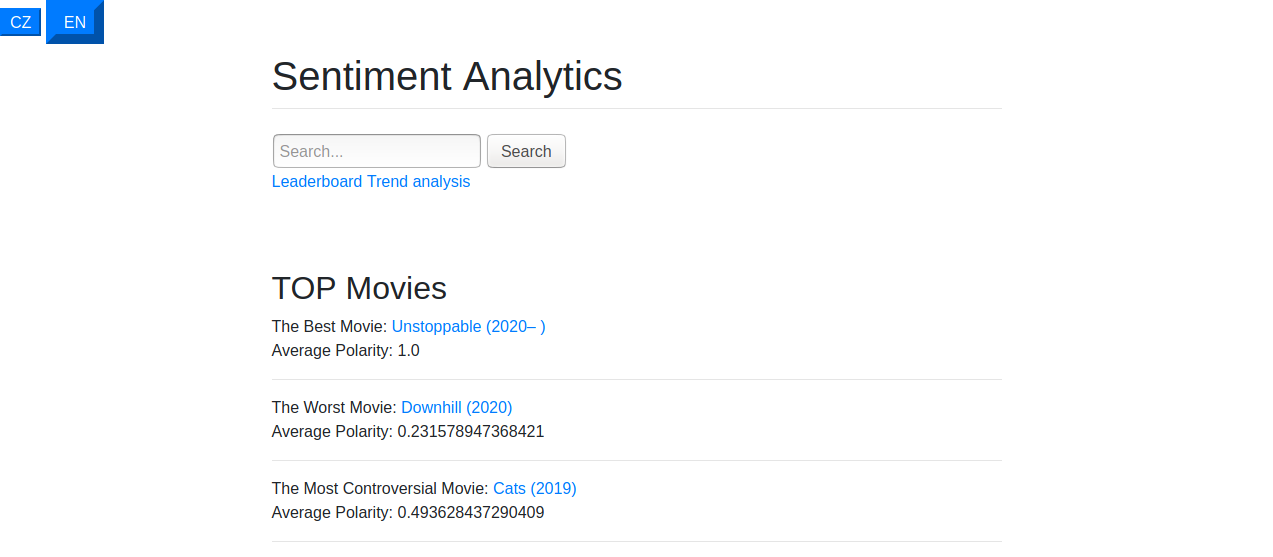
\includegraphics[width=\textwidth]{homepage.png}
\caption{Domovská stránka webového rozhraní.}
\end{figure}
\FloatBarrier
Obrázek \ref{homepg} ukazuje vzhled domovské stránky. V levém horním rohu jsou tlačítka pro přepnutí jazyka stránek. Celý systém je implementován pro češtinu i angličtinu, proto je i~zde možnost přepínat jazyky. Přepnutí jazyka změní text na stránkách i data dotazovaná z databáze. Stránky přepnuté do češtiny využívají pouze data získaná z českých zdrojů.

Domovská stránka nabízí vyhledávací okno, vyhledávat se dají tituly podle jejich názvu. Výsledkem vyhledávání je seznam všech titulů, jejichž název obsahuje hledaný výraz. Ke každému z vyhledaných filmů je připsána jeho popularita (celkový počet recenzí v databázi). 

Dále je na stránce tlačítko pro přejití na žebříček titulů, pod ním je seznam top filmů. Tlačítko pro přejití na stránku analýzy trendů je přítomno pouze pokud je stránka přepnuta do angličtiny. Analýza trendů se pro češtinu neprovádí.  

\pagebreak
\subsection{Žebříček}
\FloatBarrier
\begin{figure}[!htb]
\label{leaderb}
\centering
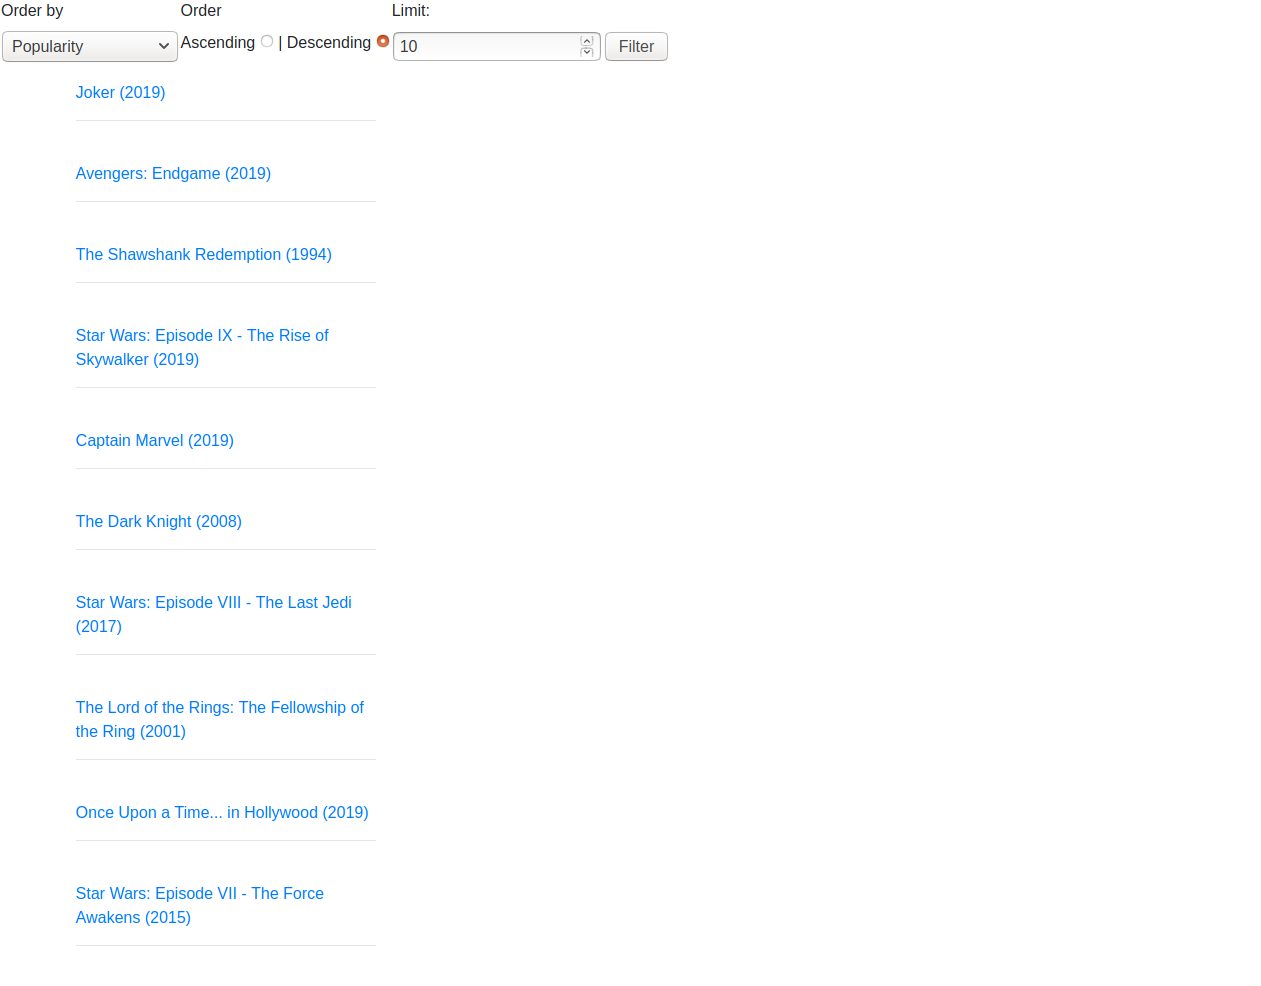
\includegraphics[width=\textwidth]{leaderboard.png}
\caption{Žebříček nejlepších / nejhorších titulů.}
\end{figure}
\FloatBarrier
Jak je vidět na obrázku \ref{leaderb}, žebříček nabízí limitovaný seznam titulů seřazených vzestupně nebo sestupně podle jednoho z následujících parametrů (hodnoty z tabulky movies):
\begin{itemize}
  \item Průměrná polarita.
  \item Průměrný počet hvězd.
  \item Popularita.
  \item Průměrné hodnoty jednotlivých aspektů. 
\end{itemize}
Celkově je tedy možnost řadit tituly podle jednoho z osmi parametrů. Limit počtu zobrazených titulů je samozřejmě nastavitelný. 

\pagebreak
\subsection{Detail filmu}
\label{moviedetail}
\FloatBarrier

\begin{figure}[!htb]
\label{movied}
\centering
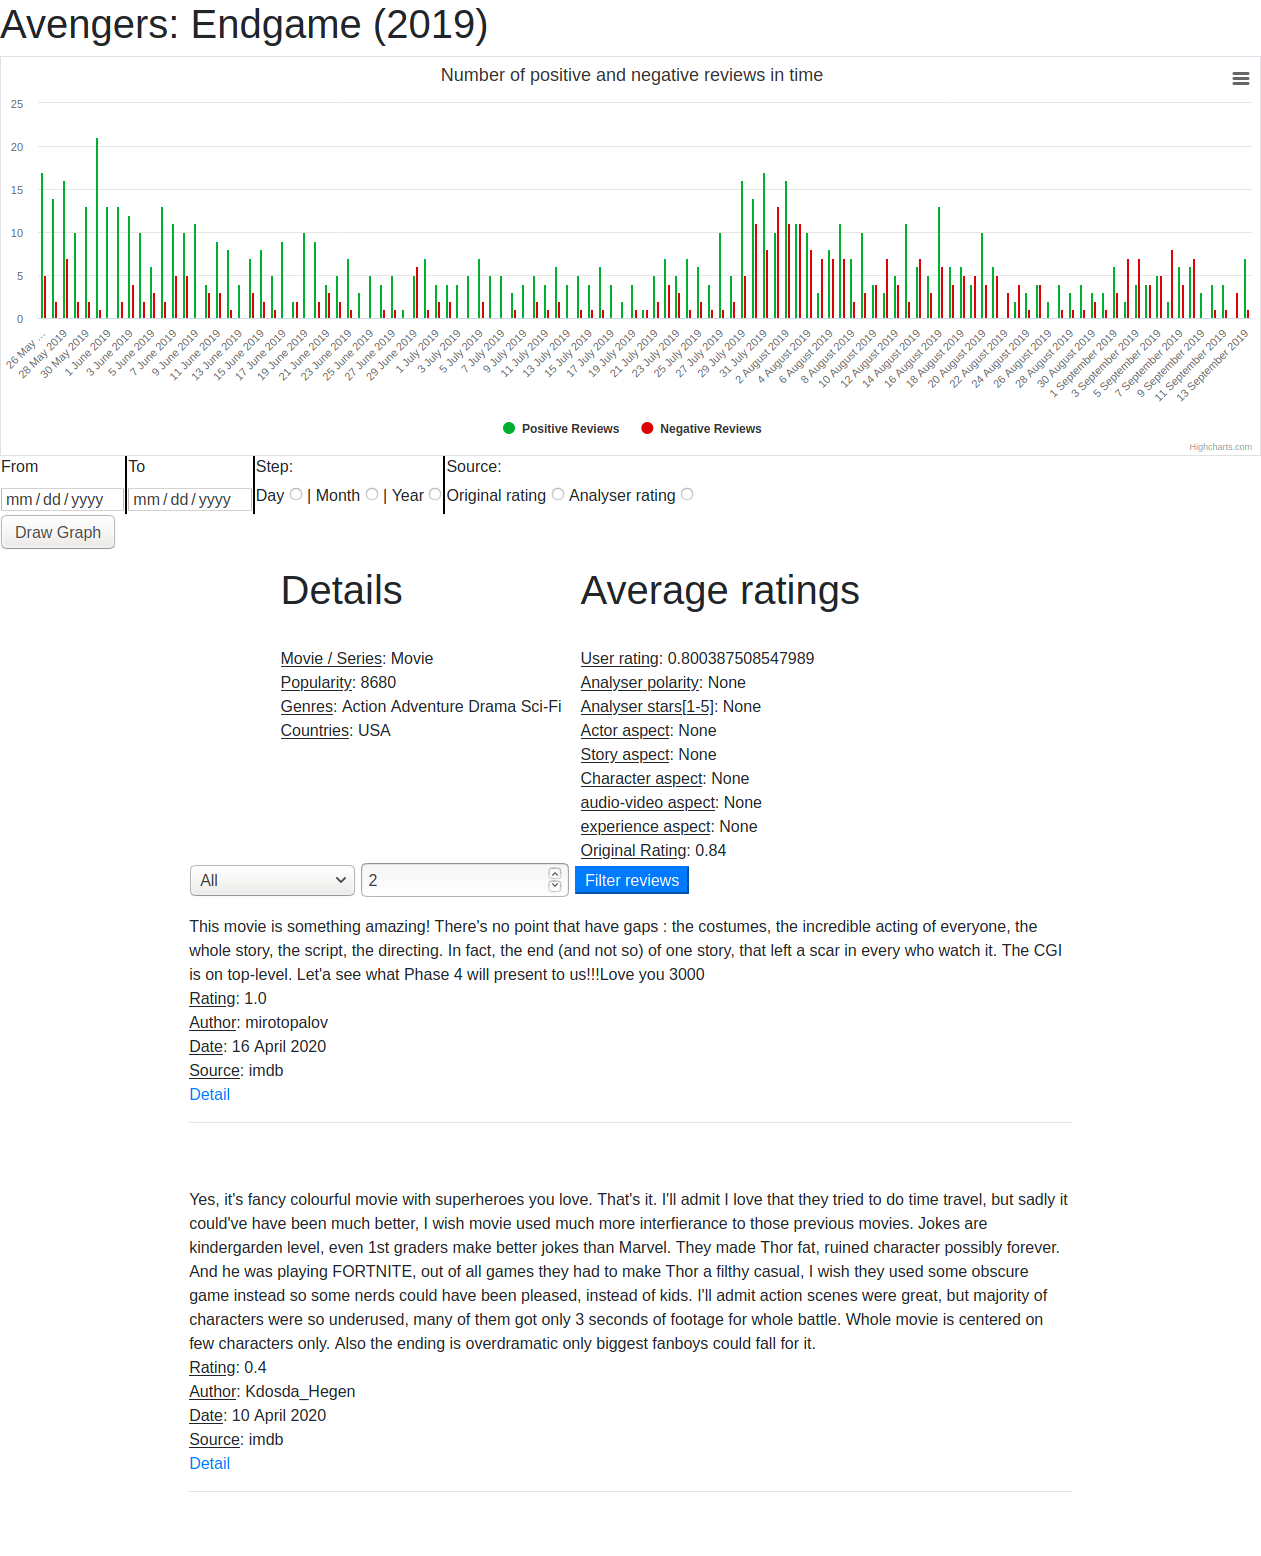
\includegraphics[width=\textwidth]{movie_detail.png}
\caption{Detailní informace o filmu.}
\end{figure}
\FloatBarrier
Stránka zobrazující detaily o filmu je na obrázku \ref{movied}. V horní sekci stránky je graf zobrazující názor na titul v čase. Nastavením grafu lze měnit časový interval i jeho krok. Dále lze nastavit zdroj názorů na daný film, první možností je originální hodnocení uživatelů, druhou možností jsou výsledky polaritní analýzy.

Ve spodní sekci stránky jsou jednotivé recenze k danému filmu. Ty je možné filtrovat podle aspektu o kterém recenze hovoří. Opět je možnost limitovat maximální počet zobrazených recenzí. 

\subsection{Detail recenze}
\FloatBarrier
\begin{figure}[!htb]
\label{reviewd}
\centering
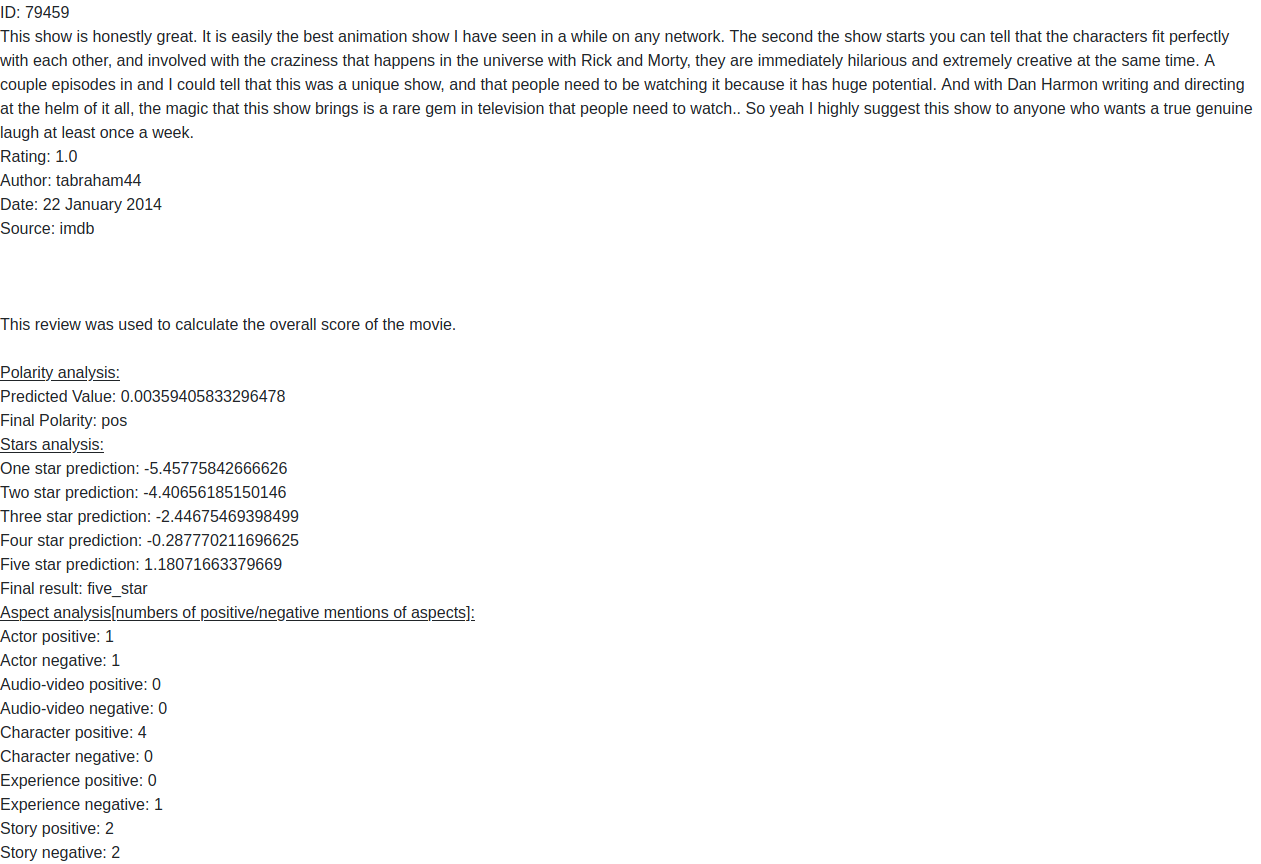
\includegraphics[width=\textwidth]{reviewdetail.png}
\caption{Detailní informace o recenzi.}
\end{figure}
\FloatBarrier
Stránka detailů recenze je na obrázku \ref{reviewd}. Obsahuje všechny detaily týkající se dané recenze. Pokud byla recenze již analyzována, obsahuje také výsledky analýz.

\pagebreak
\subsection{Analýza trendů}
\FloatBarrier
\begin{figure}[!htb]
\centering
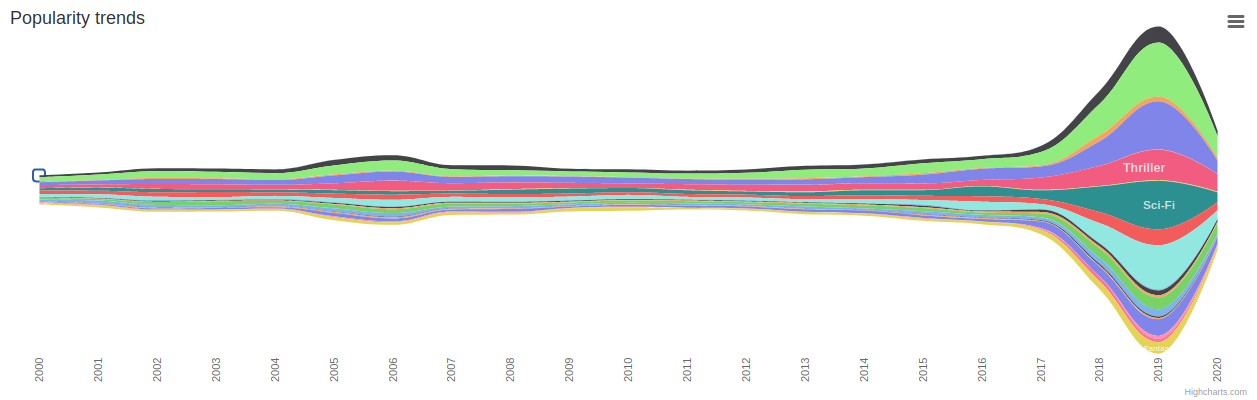
\includegraphics[width=\textwidth]{genres.png}
\label{trend}
\caption{Graf trendů popularity.}
\end{figure}
\FloatBarrier
Stránka obsahuje graf trendu popularity v čase (obrázek \ref{trend}). Popularita je zde definována jako celkový počet recenzí v databázi. Vykreslování grafu je opět nastavitelné. Krok grafu je vždy jeden rok, trendy nemá moc smysl sledovat v menším měřítku. Popularitu je možné sledovat podle typu titulu (film / seriál), podle žánru a podle země původu.


  \chapter{Vyhodnocení systému}
\label{vysledky}

Tato kapitola popisuje způsob vyhodnocení vytvořeného systému a jeho výsledky. Vyhodnocování přesnosti analyzátorů proběhlo experimentálně. Součástí této kapitoly jsou experimenty se systémem, kterými se snažím zjistit další informace, jako například schopnost systému analyzovat data z jiných domén. Pro tento systém je velice důležitý dostatek dat, proto je zde jejich množství sepsané a porovnané. Poslední část demonstruje použití vytvořeného systému.

Výsledky jsou porovnány s dalšími dostupnými publikacemi.


\section{Datová sada}


Celkově se podařilo nasbírat poměrně velké množství recenzí. Pro porovnání s dalšími publikacemi, tato česká práce \cite{cz_dataset} používá datovou sadu o velikosti 21 tisíc recenzí, anglická~\cite{en_dataset} používá 50 tisíc recenzí. Datová sada použita v anglické práci je tvořena recenzemi z~\emph{imdb.com}, tato datová sada je pro analýzu sentimentu využívána velice často, knihovna \emph{Pytorch} má vytvořenou třídu pro stažení a práci s touto datovou sadou. Mými zdroji dat byly weby \emph{čsfd.cz} a \emph{fdb.cz} pro české recenze. Zdroji anglických recenzí se staly weby \emph{imdb.com} a \emph{rottentomatoes.com}. Celkové počty nasbíraných recenzí z každého portálu jsou sepsány v~tabulce~\ref{tab:table1.1}. 

Data byla po jejich získání ukládána do databáze (tabulka \emph{reviews}). Pro trénování analyzátorů byla data uložena do lokálního souboru ve formátu JSON. Z databáze byly použity pouze záznamy, které měly neprázdný text recenze a obsahovaly číselné hodnocení autora.

Recenze byly ze všech webových portálů stahovány s číselným hodnocením autora recenze. Tyto hodnocení byly nejprve normalizovány na desetinné číslo od nuly po jedničku. Recenze byly dále rozděleny podle tohoto hodnocení na pozitivní a negativní. Negativní recenze byly všechny ty, které měly hodnocení menší nebo rovno 0.5. Pozitivní byly ty, které měly hodnocení větší než 0.5. Tímto byla vytvořena datová sada pro analyzátor polarity (pozitivní / negativní). 

Stejná data byla využita i pro vytvoření datové sady pro klasifikátor míry pozitivity (jedna až pět hvězdiček). Jednotlivé recenze byly rozděleny do pěti kategorií podle uživatelského hodnocení s krokem 0.2. 

Recenze byly dále rozděleny na trénovací (60\%), validační (15\%) a testovací (25\%). Validační data jsou využita již při trénování ke zjištění přesnosti (\emph{accuracy}) a ztráty (\emph{loss}). Tyto hodnoty jsou využity k vybrání epochy ve které byl model nejúspěšnější, tento model je uložen. Testovací data jsou použita až na konci trénování k detailnějšímu přehledu o~úspěšnosti modelu.

Všechny recenze jsou uloženy v původním stavu, předzpracovány jsou až v průběhu trénování / analýzy.




\FloatBarrier
\begin{table}[h!]
  \begin{center}
    \caption{Počet recenzí pro polaritní analyzátor a analyzátor míry polarity}
    \label{tab:table1.1}
    \begin{tabular}{l|r|r|r}
      \textbf{Zdroj} & \textbf{Pozitivní} & \textbf{Negativní} & \textbf{Celkem}\\ 
      \hline
      \textbf{IMDb} & 1\,811\,198 & 855\,672 & 2\,666\,870\\ 
      \textbf{Rotten Tomatoes} & 5\,098 & 74\,270 & 79\,368 \\ 
      \textbf{ČSFD} & 239\,290 & 758\,021 & 997\,311\\ 
      \textbf{FDb} & 37\,055 & 108\,562 & 145\,617\\ 
      \textbf{Celkem} & 2\,092\,641 & 1\,796\,525 & 3\,889\,166\\ 
    \end{tabular}
  \end{center}
\end{table}
\FloatBarrier
\FloatBarrier

Data pro aspektové analyzátory byly anotovány ručně, proto jich je také mnohem méně, konkrétní počty v tabulkách \ref{tab:table1.2} pro češtinu a \ref{tab:table1.3} pro angličtinu. Opět pro srovnání, tato práce \cite{en_dataset2} má pro angličtinu čtyři datové sady, každá okolo 2\,000 vět.

Datová sada byla vytvořena následovně, nejprve byly vybrány náhodné recenze, poté byly rozděleny na věty pomocí nástrojů \emph{spacy} a \emph{nltk}. Jednotlivé věty byly ručně označeny pomocí nástroje \emph{brat}, který běží v prohlížeči. Server pro tento nástroj byl spouštěn lokálně na mém počítači. Každá věta byla anotována žádným až pěti aspekty a polaritou daného aspektu. Takto anotovaná data byla použita pro trénování analyzátorů polarity aspektů. Pro vytvoření datové sady k trénování analyzátorů detekujících aspekty ještě byly doplněny náhodné věty, datová sada pro analyzátory detekující aspekt byla tedy oproti hodnotám v~tabulkách dvakrát větší. 

\begin{table}[h!]
  \begin{center}
    \caption{Počet vět pro klasifikátory polarity aspektů v češtině}
    \label{tab:table1.2}
    \begin{tabular}{l|r|r|r}
      \textbf{Aspekt} & \textbf{Pozitivní} & \textbf{Negativní} & \textbf{Celkem}\\ 
      \hline
      \textbf{Herec} & 127 & 107 & 234\\ 
      \textbf{Postava} & 69 & 69 & 138 \\ 
      \textbf{Audio vizuální efekty} & 97 & 78 & 175\\ 
      \textbf{Příběh} & 81 & 81 & 162\\ 
      \textbf{Zkušenost} & 79 & 83 & 162\\ 
      \textbf{Celkem} & 453 & 418 & 871\\ 
    \end{tabular}
  \end{center}
\end{table}
\FloatBarrier
\begin{table}[h!]
  \begin{center}
    \caption{Počet vět pro klasifikátory polarity aspektů v angličtině}
    \label{tab:table1.3}
    \begin{tabular}{l|r|r|r}
      \textbf{Aspekt} & \textbf{Pozitivní} & \textbf{Negativní} & \textbf{Celkem}\\ 
      \hline
      \textbf{Herec} & 125 & 127 & 252\\ 
      \textbf{Postava} & 89 & 92 & 181 \\ 
      \textbf{Audio vizuální efekty} & 107 & 99 & 206\\ 
      \textbf{Příběh} & 164 & 168 & 332\\ 
      \textbf{Zkušenost} & 104 & 107 & 211\\ 
      \textbf{Celkem} & 589 & 593 & 1\,182\\ 
    \end{tabular}
  \end{center}
\end{table}
\FloatBarrier


\section{Maximální dosažená přesnost}
V této sekci jsou porovnány maximální dosažené přesnosti všech prováděných analýz vzhledem k použité metodě. Analyzátory byly trénovány na dříve popsaných datových sadách. Pro trénování analyzátorů založených na neuronové síti se data vybalancovala a rozdělila na trénovací, testovací a validační sady. Využita byla tedy většina dat. Oproti tomu při trénování analyzátorů založených na metodě podpůrných vektorů a naivní Bayesovské metodě, jsem byl z důvodu paměťové náročnosti způsobu trénování nucen vždy použít jen část trénovacích dat. 

Sledována je pouze přesnost (\emph{accuracy}) analyzátorů, která je definována jako poměr mezi počtem správných předpovědí (\emph{true positive}$+$\emph{true negative}) a celkovým počtem testovacích příkladů. Recenze byly před trénováním i testováním předzpracovány stejně jako bylo popsáno v kapitole \ref{implementace}. 

Snažím se zde odpovědět na otázku, zda-li je vůbec při analýze recenzí nutné používat relativně komplikovanější a náročnější metody jako jsou neuronové sítě, nebo stačí jednodušší metody jako podpůrné vektory nebo naivní Bayesova.




\subsection{Analýza polarity}

Prvním testovaným analyzátorem je analyzátor polarity. Analyzuje na úrovni celého dokumentu (recenze) a přiřazuje mu pozitivní nebo negativní třídu.
\FloatBarrier
\begin{table}[h!]
  \begin{center}
    \caption{Maximální přesnost použitých metod}
    \label{tab:table1.4}
    \begin{tabular}{l|l|l}
      \textbf{Metoda} &  \multicolumn{2}{l}{\textbf{Přesnost (\emph{Accuracy})}}\\ 
      \hline
      \textbf & CZ & EN \\ 
      \textbf{Neuronová síť (oboustranné LSTM)} & 0.81 & 0.88  \\ 
      \textbf{Metoda podpůrných vektorů} & 0.80 & 0.83 \\ 
      \textbf{Naivní Bayesovská metoda} & 0.69 & 0.69 \\ 
     \end{tabular}
  \end{center}
\end{table}
Z tabulky \ref{tab:table1.4} je patrné, že nejvyšší přesnost má dle očekávání systém založený na hlubokém učení. Z tohoto důvodu byl zvolen pro automatizovanou analýzu recenzí. Tento klasifikátor (obzvlášť pro angličtinu) dosáhl poměrně vysoké přesnosti, za nejmodernějšími systémy však ještě zaostává. Nejlepších výsledků by se pravděpodobně dosáhlo využitím systému jako je BERT a jeho doladěním na doménu filmových recenzí. Chtěl jsem si však klasifikátor z osobních důvodů implementovat sám, proto jsem se vydal touhle cestou.

Porovnáním přesností lze vidět, že metoda podpůrných vektorů moc nezaostává a její přesnost by byla přijatelná. V tomto případě by tedy asi nebyla potřeba využívat komplikovanějších metod.  
\FloatBarrier


\subsection{Analýza míry pozitivity}
Druhým typem analyzátoru je analyzátor míry pozitivity. Také analyzuje na úrovní dokumentu, přiřazuje jednu z pěti tříd (jedna až pět hvězd).
\FloatBarrier
\begin{table}[h!]
  \begin{center}
    \caption{Maximální přesnost použitých metod}
    \label{tab:table1.5}
    \begin{tabular}{l|l|l}
      \textbf{Metoda} &  \multicolumn{2}{l}{\textbf{Přesnost (\emph{Accuracy})}}\\ 
      \hline
      \textbf & CZ & EN \\ 
      \textbf{Neuronová síť (oboustranné LSTM)} & 0.62 & 0.55  \\ 
      \textbf{Metoda podpůrných vektorů} & 0.46 & 0.53 \\ 
      \textbf{Naivní Bayesovská metoda} & 0.45 & 0.52 \\ 
     \end{tabular}
  \end{center}
\end{table}
\FloatBarrier
Pro automatizovanou analýzu je opět používán analyzátor založený na hlubokém učení kvůli jeho přesnosti. Ostatní metody však moc nezaostávají, takže by byly použitelné také. Hned na první pohled lze v tabulce \ref{tab:table1.5} vidět, že oproti analýze polarity mají všechny metody přesnost nižší. To se dá očekávat, protože tento typ klasifikace je obtížnější. 
Z~důvodu poměrně velké změny v přesnosti jsem se však rozhodl analyzovat chyby hlouběji. Analýza chyb byla provedena na anglické datové sadě s využitím klasifikátoru založeném na hlubokém učení.
Celkový počet testovacích příkladů byl 146\,664, z toho bylo 60\,565 chyb (to znamená přesnost 0.58). U každé chyby bylo zaznamenáno, jestli se klasifikátor dopustil chyby pouze o jednu hvězdu nebo více. Výsledky jsou následující (nalevo od pomlčky je předpokládaná odpověď analyzátoru).

\textbf{Počet chyb o jednu hvězdu:}
\begin{itemize}
    \item jedna hvězda - 792
    \item dvě hvězdy - 4\,132
    \item tři hvězdy - 10\,404
    \item čtyři hvězdy - 4\,921
    \item pět hvězd - 9\,361
\end{itemize}

\textbf{Počet chyb o více než jednu hvězdu:}
\begin{itemize}
    \item jedna hvězda - 4\,434
    \item dvě hvězdy - 9\,890
    \item tři hvězdy - 6\,324
    \item čtyři hvězdy - 7\,960
    \item pět hvězd - 2\,347
\end{itemize}

Celkově bylo 29\,610 chyb o jednu hvězdu, to je 48\,\% všech chyb. Předpokládám, že tohle je z důvodu malého rozdílu v obsahu textu recenzí mezi těmi blízko u sebe v hodnocení.

\FloatBarrier

\subsection{Analýza aspektů}
Aspektová analýza se skládá ze dvou úkolů, detekci aspektu (výsledky v tabulce \ref{tab:table1.6}) a~určení polarity daného aspektu (tabulka \ref{tab:table1.7}).
\FloatBarrier
\begin{table}[h!]
  \begin{center}
    \caption{Detekce aspektu}
    \label{tab:table1.6}
    \begin{tabular}{l|l|l}
      \textbf{Metoda} &  \multicolumn{2}{l}{\textbf{Přesnost (\emph{Accuracy})}}\\ 
      \hline
      \textbf & CZ & EN \\ 
      \textbf{Neuronová síť (oboustranné LSTM)} & 0.72 & 0.71  \\ 
      \textbf{Metoda podpůrných vektorů} & 0.74 & 0.73 \\ 
      \textbf{Naivní Bayesovská metoda} & 0.72 & 0.66 \\ 
     \end{tabular}
  \end{center}
\end{table}
\FloatBarrier


\begin{table}[h!]
  \begin{center}
    \caption{Určení polarity aspektu}
    \label{tab:table1.7}
    \begin{tabular}{l|l|l}
      \textbf{Metoda} &  \multicolumn{2}{l}{\textbf{Přesnost (\emph{Accuracy})}}\\ % <-- added & and content for each column
      %$\alpha$ & $\beta$ & $\gamma$ & $\delta$ \\ % <--
      \hline
      \textbf & CZ & EN \\ 
      \textbf{Neuronová síť (oboustranné LSTM)} & 0.69 & 0.69  \\ 
      \textbf{Metoda podpůrných vektorů} & 0.65 & 0.68 \\ 
      \textbf{Naivní Bayesovská metoda} & 0.64 & 0.67 \\ 
     \end{tabular}
  \end{center}
\end{table}
\FloatBarrier

Na české datové sadě byla přesnost zjištěna pro aspekt \uv{herec}, na anglické pro aspekt \uv{příběh}. Tyto aspekty byly vybrány, protože mají nejvíce anotovaných vět. Důvodem je nutnost rozdělení datových sad na trénovací a testovací části. Klasifikátory ostatních aspektů mají velice podobnou přesnost.

Z výsledků je patrné, že všechny metody mají velice podobné výsledky. Tohle je způsobeno menším počtem dat. Pro automatickou analýzu je opět zvolena neuronová síť. 

\section{Využití analyzátorů v jiných doménách}
Těmito experimenty je testována schopnost polaritních analyzátorů pracovat na datech z~jiných domén. Filmových recenzí je obrovské množství, navíc jsou již anotovány autorem. Kdyby se tedy ukázalo, že analyzátory natrénované na těchto datech jsou úspěšné i v jiných doménách, mohlo by  to ulehčit práci s hledáním trénovacích dat.  Testy byly provedeny na následujících datových sadách (vyvážená byla pouze sada Mallcz):
\begin{itemize}
    \item Facebook - česká datová sada, necelých 5\,000 příspěvků.
    \item Mallcz - česká datová sada, použito 10\,000 recenzí.
    \item Hudební nástroje - anglická datová sada, jedná se o recenze z webového portálu \emph{Amazon}. Přes 10\,000 recenzí.
    \item Automobilový průmysl - anglická datová sada, jedná se o recenze z webového portálu \emph{Amazon}. Přes 20\,000 recenzí.
    \end{itemize}

\FloatBarrier
\begin{table}[h!]
  \begin{center}
    \caption{Polaritní analyzátory v jiných doménách}
    \label{tab:table1.8}
    \begin{tabular}{l|l|l|l|l}
      \textbf{Metoda} &  \multicolumn{4}{l}{\textbf{Přesnost (\emph{Accuracy})}}\\ % <-- added & and content for each column
      %$\alpha$ & $\beta$ & $\gamma$ & $\delta$ \\ % <--
      \hline
      \textbf & Facebook & Mallcz & Hudební nástroje & Automobilový průmysl \\ 
      \textbf{Neuronová síť} & 0.57 & 0.51 & 0.83 & 0.75  \\ 
      \textbf{Podpůr. vekt.} & 0.52 & 0.47 & 0.77 & 0.59 \\  \textbf{Naivní Bayes.} & 0.43 & 0.45 & 0.14 & 0.12 \\ 
     \end{tabular}
  \end{center}
\end{table}
\FloatBarrier
Ve výsledcích jde vidět (tabulka \ref{tab:table1.8}), že obecně jsou úspěšnější anglické datové sady. To bude pravděpodobně tím, že čeština je bohatější jazyk a tím těžší pro klasifikátor na naučení. 

Přesnost naivní bayesovské metody v anglických datových sadách je opravdu zvláštní. Všechno bylo zkontrolováno, test byl proveden několikrát a vždy vyšel stejně. 

Z výsledků vyplývá, že analyzátory kromě třech případů nejsou velice úspěšné. Filmové recenze jsou nejspíše příliš konkrétní doménou a pro trénování analyzátorů do jiných domén se moc nehodí. Klasifikátory by se daly doladit (dotrénovat na konkrétní doméně) a tím zvýšit jejich přesnost. Toto už však testováno nebylo.  

\FloatBarrier

\section{Přesnost v závislosti na velikosti trénovacích dat}
Zde chci porovnat přesnosti metod polaritní analýzy v závislosti na počtu trénovacích příkladů. Cílem je zjistit potřebné množství dat pro natrénovaní analýzátoru s přijatelnou přesností. Využity jsou části již popsaných datových sad. Testování probíhalo na náhodně vybrané sadě o velikosti 100\,000 recenzí. Trénovací sada (také vytvořená náhodně) se postupně zvětšovala. 

\FloatBarrier
\begin{table}[h!]
  \begin{center}
    \caption{Přesnost v závislosti na velikosti trénovacích dat}
    \label{tab:table1.9}
    \begin{tabular}{r|r|r|r|r|r|r}
      \textbf{Počet recenzí} &  \multicolumn{2}{l}{\textbf{Neuronová síť}} & \multicolumn{2}{l}{\textbf{SVM}} & \multicolumn{2}{l}{\textbf{Bayes}}\\ 
      \hline
      \textbf & CZ & EN & CZ & EN & CZ & EN \\ 
      \textbf{50} & 0.65 & 0.54 & 0.66 & 0.69 & 0.54 & 0.52  \\ 
      \textbf{100} & 0.66 & 0.46 & 0.67 & 0.71 & 0.62 & 0.66 \\  
      \textbf{200} & 0.70 & 0.62 & 0.77 & 0.70 & 0.71 & 0.64 \\ 
      \textbf{500} & 0.70 & 0.67 & 0.78 & 0.76 & 0.72 & 0.67 \\ 
      \textbf{1000} & 0.72 & 0.65 & 0.77 & 0.77 & 0.74 & 0.68 \\ 
      \textbf{2000} & 0.72 & 0.66 & 0.80 & 0.78 & 0.72 & 0.68 \\ 
      \textbf{5000} & 0.74 & 0.68 & 0.79 & 0.80 & 0.73 & 0.69 \\ 
      \textbf{10000} & 0.78 & 0.75 & 0.81 & 0.80 & 0.75 & 0.71 \\ 
     \end{tabular}
  \end{center}
\end{table}
\FloatBarrier

V tabulce \ref{tab:table1.9} jde vidět, že po trénování na datové sadě o velikosti 5\,000 recenzí již za svým maximem zaostává pouze klasifikátor založený na neuronové síti. Z toho vyplývá, že pro menší datové sady je lepší využít jiné metody. 

Cekově z výsledků vyplývá, že pro natrénování poměrně přijatelně přesného klasifikátoru není potřeba příliš mnoho dat (v poměru k počtu dostupných recenzí). 

\section{Demonstrace systému}
V této sekci chci ukázat několik příkladů jak se dá vytvořený systém využít a jaké informace se dají za jeho pomoci získat. 


\subsection{Správné vydání filmu}

Pro analýzu dat byl použit dříve popsaný graf polarity (kapitola \ref{moviedetail}). 
\begin{figure}[!htb]
\label{ad_astra}
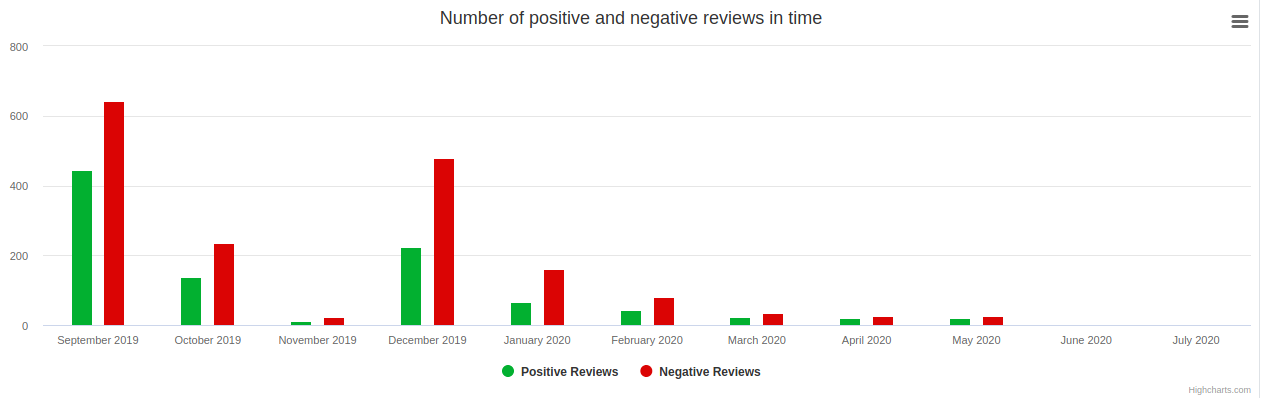
\includegraphics[width=\textwidth]{ad_astra.png}
\caption{Počet pozitivních a negativních hodnocení v čase pro film \emph{Ad Astra}}
\end{figure}

\begin{figure}[!htb]
\label{cats}
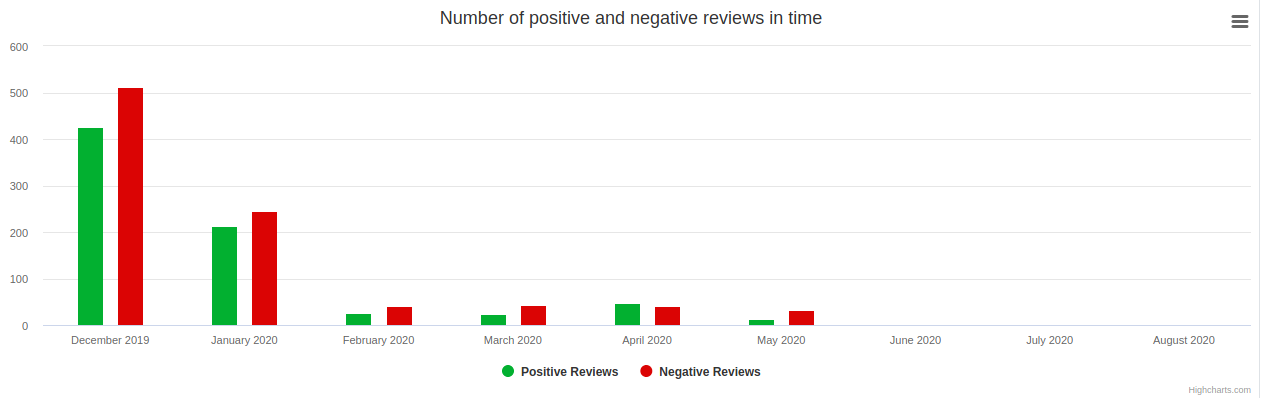
\includegraphics[width=\textwidth]{cats.png}
\caption{Počet pozitivních a negativních hodnocení v čase pro film \emph{Cats}}
\end{figure}

Oba filmy jsou poměrně neúspěšné, celkové hodnocení mají okolo 50\,\%. Pohledem na oba grafy \ref{ad_astra} a \ref{cats} lze zjisti, že jejich průběhy jsou velice podobné. Po vydání poměrně vysoká popularita (velký počet pozitivních i negativních recenzí). Po čase však tato popularita rapidně klesá. Pohledem na graf \ref{ad_astra} lze vidět v prosinci 2019 velký nárůst popularity. Po krátkém zkoumání lze zjistit, že v tomto měsíci byl film vydán na DVD, to je zhruba 3~měsíce po vydání. Tento fakt velice pozvedl popularitu. Oproti tomu film \emph{Cats} (graf \ref{cats}) žádný takový nárůst nemá. DVD tohoto filmu bylo totiž vydáno až téměř po půl roce od vydání, podle grafů tohle byla chyba. Po tak dlouho době již vyprší nadšení z nového filmu a jeho marketingové kampaně.  



\subsection{Pravdivost celkových hodnocení}
U převážné většiny titulů je originální celkové hodnocení a celkové hodnocení vytvořené systémem velice podobné. Zde prezentuji jeden příklad kdy tohle není pravdou. 

\begin{figure}[!htb]
\label{starwars}
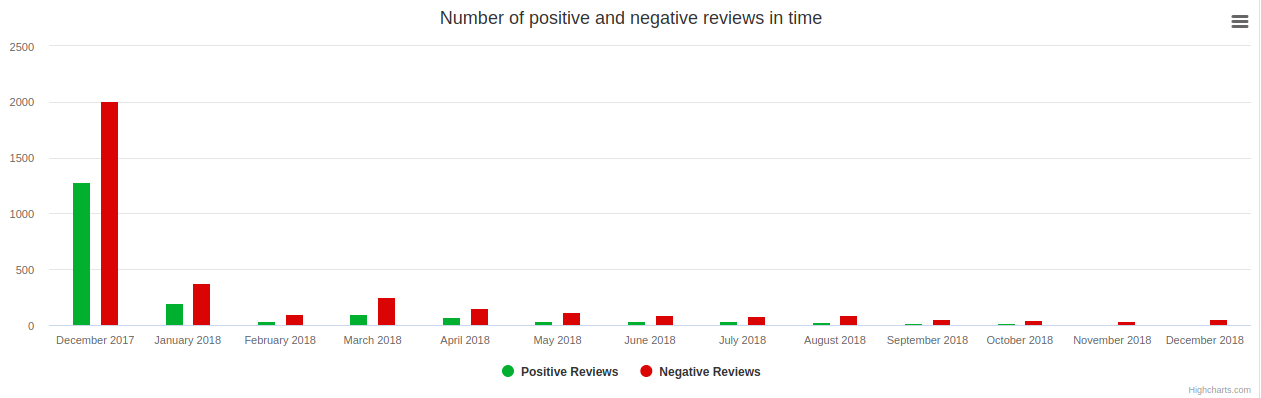
\includegraphics[width=\textwidth]{last_jedi.png}
\caption{Počet pozitivních a negativních hodnocení v čase pro film \emph{Star Wars: Episode VIII - The Last Jedi (2017)}}
\end{figure}

Již na první pohled lze v grafu \ref{starwars} vidět, že se nejedná o velice úspěšný film. Celkové hodnocení systému(vytvořené průměrem hodnocení uživatelů \emph{imdb}) je 41\,\%. Při návštěvě webových stránek \emph{imdb} však vidíme hodnocení 7/10. Velice podobný případ lze nalézt i~u~2~roky staršího předchůdce \emph{Star Wars: Episode VII - The Force Awakens}. Tam systém tvrdí 57\,\%, na \emph{imdb} je však napsáno 7,9/10.



\chapter{Závěr}
\label{zaver}

Cílem této práce bylo navrhnout a implementovat systém schopný pravidelně získávat, indexovat a analyzovat recenze filmů v češtině a angličtině. Cíl práce byl splněn. 

V práci je prostudována teorie základních i pokročilých metod pro rozpoznávání postojů a zpracování přirozeného jazyka. Dále byly určeny vhodné zdroje recenzí filmů a seriálů pro oba jazyky. Těmito zdroji se staly webové portály \emph{csfd.cz}, \emph{fdb.cz}, \emph{imdb.com} a \emph{rottentomatoes.com}. Recenze z těchto portálů jsou pravidelně stahovány a indexovány v relační databázi. Současně jsou v databázi téměř čtyři miliony recenzí filmů a seriálů. 

Využitím těchto recenzí byly natrénovány analyzátory třech typů. Prvním z nich je analyzátor polarity na úrovni dokumentu určující celkový postoj recenze (pozitivní / negativní). Tento analyzátor dosahuje přesnosti až 88\,\% pro angličtinu a 81\,\% pro češtinu. Druhým typem je analyzátor míry pozitivity pracující také na úrovni dokumentu, tento analyzátor rozděluje recenze do pěti tříd (jedna až pět hvězd). Tato analýza dává detailnější informace o recenzi, ale má nižší přesnost, a to 55\,\% pro angličtinu a 62\,\% pro češtinu. Po detailnější analýze chyb toho klasifikátoru se ukázalo, že má problém s rozlišením recenzí s podobným hodnocením (například recenze s pěti a čtyřmi hvězdičkami). Posledním typem je analýza aspektů, která dává nejdetailnější informace. Předem bylo definováno pět aspektů, které jsou u recenzí sledovány (herec, postava, příběh, audio vizuální efekty a zkušenost diváka). Analýza je rozdělena do dvou kroků, nejprve jsou jednotlivé aspekty nalezeny a poté ohodnoceny polaritou (pozitivní / negativní).

Výsledky z automaticky prováděných analýz jsou ukládány do relační databáze a zobrazovány ve webovém rozhraní (\url{http://athena1.fit.vutbr.cz:8078/}). Rozhraní uživateli nabízí vyhledávat a filtrovat filmy a seriály. Každý film má vytvořenou časovou osu názorů na daný film s detailní analýzou jednotlivých recenzí týkajících se filmu. Dále jsou sledovány trendy titulů podle žánru, země původu a jestli je daný titul film či seriál. 

V práci bych pokračoval anotací dalších dat pro aspektovou analýzu, tím by se zvýšila její přesnost, popřípadě bych otestoval další metody implementace analyzátorů. Dále bych rád udělal hezčí a dynamičtější webové rozhraní. Pro přilákání uživatelů na platformu by bylo dobré jim dát možnost přímo interagovat s klasifikátory, dnes je téma strojového učení velice populární.    
  %% Tento soubor nahraďte vlastním souborem s obsahem práce.
%=========================================================================
% Autoři: Michal Bidlo, Bohuslav Křena, Jaroslav Dytrych, Petr Veigend a Adam Herout 2019
\chapter{Úvod}
Zde bude cca jedna strana úvod…

\blindtext[2]
\todo{Upravit}.


\chapter{Automatizace domácnosti}
Následující část je shrnutím současného stavu v oblasti automatizace domácnosti a chytrých domovů. Není encyklopedickým výkladem problematiky, ale souhrnem informací, které mají k práci bezprostřední vztah. Nejprve je zde popis automatizace domácnosti, co to je, jaké jsou dnes možnosti jejího využití, přínosy a používané principy.

\section{Automatizace domácnosti a chytrý dům}
Automatizace domácnosti spočívá v automatizování činností, které řídí domácnost, normálně vykonávané člověkem. Můžeme ji definovat jako mechanismus, který nahrazuje lidskou námahu (při ovládání domácnosti), natolik, nakolik je to jen možné [U]. V souvislosti s tím někdy hovoříme o inteligentní, řízené či chytré domácnosti. Jedná se o kolekci zařízení a (pod)systémů, které jsou schopny spolu komunikovat či fungovat nezávisle. Přitom automatizovaný „dům budoucnosti“ slibují výrobci domácích zařízení prakticky již téměř od počátku minulého století [1]. Chytrý dům (či smart home) je pak definován jako dům, vybavený výpočetní a informační technologií, které předvídá uživatelovi potřeby a odpovídá na ně, a přitom dbá na jeho pohodlí, bezpečnost a zábavu [13]. Často se tedy tyto dva pojmy (automatizovaný a chytrý dům) zaměňují, ačkoli \todo{Z nějakého nového zdroje rozvést, viz odkaz}
\begin{verbatim}
https://www.google.com/search?q=smart+home+vs+home+automation&rlz=1C1AVFC_enCZ780CZ780&oq=smart+home+vs+hom&aqs=chrome.0.0i19j69i57j0i19i22i30j0i5i13i19i30l5.7375j0j7&sourceid=chrome&ie=UTF-8
\end{verbatim}




\subsection*{Možnosti využití automatizace v domácnosti}
Automatizace v mnohém usnadňuje život a umožňuje provádění akcí, které by jinak byli prakticky nemožné (například zabezpečení domu, efektivní řízení vytápění domácnosti a spotřeby energie). V současné době patří automatizace domácnosti mezi rychle se rozvíjející technologie \todo{Dopsat zdroj, viz  odkaz} []. 
\begin{verbatim}
https://www.google.com/search?q=home+automation+is+fast+developing&rlz=1C1AVFC_enCZ780CZ780&oq=home+automation+is+fast+deveopin&aqs=chrome.1.69i57j33i10i160.14343j0j7&sourceid=chrome&ie=UTF-8
\end{verbatim} 
Mezi typické aplikace automatizace domácnosti patří například:
\begin{itemize}
\item Zabezpečovací systém
\item Systém pro inteligentní vytápění a ventilaci (HVAC)
\item Zábava a multimédia
\item Komunikace
\item Osvětlení [3]
\item Ovládání spotřebičů [T]
\item Samo zavlažovací systémy [U]
\item A mnoho dalšího
\end{itemize}

\begin{figure}[hbt]
	\centering
	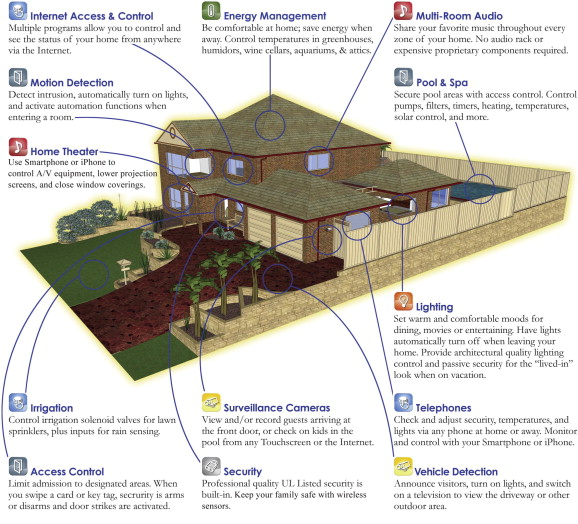
\includegraphics{obrazky/automation-example.jpg}
	\caption{Příklad možností automatizované domácnosti[U]}
	\label{asd}
\end{figure}
Nejaky text, mozna spise az sem o tom, že "V současné době patří automatizace domácnosti mezi rychle se rozvíjející technologie".


\newpage
\subsection*{Přínosy automatizace domácnosti}
Přidání inteligence do domácnosti přináší do života lidí řadu přínosů. Jde zejména o:

\begin{itemize}
\item Bezpečí – Chytré domy mohou používat různé senzory, které detekují nebezpečí a v souvislostí s nimi provést patřičné akce k jejich zabránění, případně minimalizaci škod. Příkladem mohou být záplavové a kouřové senzory a v neposlední řadě také zabezpečovací systém domácnosti.
\item Komfort – Chytré domácnosti svými funkcemi nabízejí různé způsoby, jak jejich uživatelům zpříjemnit různé rutinní akce. Mohou se postarat o automatické nastavování žaluzií dle intenzity venkovního světla, přes dotykový displej na dálku ztlumit světlo či hlasovým pokynem uvést celý byt do jiného světelného režimu. 
\item Přehled o provozu – Systémy pro automatizaci domácnosti zahrnují i displeje s přehledem o stavu jednotlivých zařízení a čidel. Také je v některých systémech možné tyto informace sledovat i z chytrých telefonů, tabletů či počítačů (a to i vzdáleně). V některých komplexnějších systémech, které například zahrnují komunikaci přes mobilní sítě je možné získávat přehled o provozu dokonce pomocí SMS zprávy (hodí se třeba při absenci internetového připojení) [15]
\item Úspora – V chytrých domácnostech je možné použít inteligentní vytápění domu založené na údajích z teplotních čidel, denní doby, případně nastaveném režimu domácnosti. Společnost ELKO EP odhaduje, že díky bezdrátové regulaci topení je možné ušetřit až 30 \% nákladů na energii [17]. Úsporu rovněž zajistí automatizovaná světla, o kterých je možné mít v automatizované domácnosti vždy přehled, na dálku je zapínat/vypínat dle potřeby a rovněž je napojit na senzory, které je budou ovládat například na základě přítomnosti osob v místnosti.
\end{itemize}
    

\subsection*{Základní klasifikace chytré domácnosti}
Chytrou domácnost můžeme rozdělit dle kabeláže:

\begin{itemize}
\item Drátovou
\item Bezdrátovou 
\item Kombinovanou
\end{itemize}
Pokud má být domácnost komplexně automatizovaná, je často vhodnější mít celý systém propojený pomocí kabelů, jelikož takový systém bude spolehlivější a v případě potřeby nabízí rychlejší přenos dat (například pokud mají být součástí systému multimédia). Bezdrátové systémy se hodí zejména tam, kde není žádané zasahovat do elektroinstalace, či pokud uživatel potřebuje pouze jednodušší systém (například s ovládáním několika málo zařízení). Připravená kabeláž pro automatizaci domácnosti rovněž přináší výhodu snadnějšího řešení napájení jednotlivých chytrých zařízení, které se tak může rozvádět po bytě spolu s datovými kabely. Přitom pro propojení jednotlivých chytrých zařízení mezi sebou je možné využít různé typy kabelů (např. ethernetový) [15]. Systémy s kombinovanou kabeláží pak vycházejí z klasické kabelové instalace s možností použití některých bezdrátových prvků (např. snímačů).


\subsection*{Mechanismy používané v chytrých domovech}
V chytrém domě se při automatizaci obvykle používají následující principy:

\begin{itemize}
\item Přímé ovládání spotřebičů
\item Nastavení scény
\item Podmínky [16, pokud neseženu lepší]
\end{itemize}
Přímé ovládání spotřebičů se obvykle provádí dálkovým ovládáním, používá-li spotřebič pro komunikaci technologii rádiového přenosu na frekvencích 443 MHz. Příkladem takového zařízení může být „bla bla bla“ od společnosti...Jiný způsob ovládání rovněž zahrnuje použití jiného chytrého zařízení (například chytrého telefonu), pokud ovládané zařízení umí komunikovat pomocí stejné technologie (např. WiFi). Ovládání pomocí telefonu či podobného chytrého zařízení je možné i v případě, že ovládané zařízení neumí komunikovat stejnou technologií, ale v domácnosti existuje centrální prvek (hub), který podporuje obě technologie a funguje zde jako prostředník mezi oběma zařízeními. \newline
V chytrých domovech je rovněž často možné použít rovněž nastavení některé předem definované scény. Tato scéna sdružuje několik příkazů přímého ovládání. Může se například jednat o scénu odchodu z domu, která vypne všechna světla, odpojí spotřebiče od elektrické sítě a aktivuje zabezpečovací systém.\newline
Dalším principem uplatňovaným v chytrém domě jsou nastavené podmínky. Ty způsobí, že při určité akci systém zareaguje nějakým předem nastaveným způsobem. Například se může jednat o podmínku, aby v případě že s….\newline

\subsection*{Komponenty chytré domácnosti}
Na trhu dnes existuje nepřeberné množství různých systémů. Typická automatizovaná domácnost využívá některé (či všechny) z následujících komponent: \newline

\begin{itemize}
\item Vstupní prvky (různá čidla, tlačítka, dotykové displeje…)
\item Výstupní prvky (Světla, spotřebiče a různá zařízení)
\item Virtuální (hlasový) asistent
\item Centrální jednotka
\item Aplikace pro řízení domácnosti z chytrých zařízení (telefonu, tabletu, počítače…)
\end{itemize}

\subsection*{Chytrá zařízení a IoT}
\todo{todo}

\subsection*{Protokoly používané v automatizaci domácnosti}
\todo{todo - MQTT atd...}
\todo{Možná změnit uplně kapitolu technol. bezdrátového přenosu na Protokoly a tam radši dát MQTT atd?}


\section{Virtuální hlasoví asistenti a centrální prvky chytré domácnosti}
Virtuální osobní asistent (VPA) je osobní asistent, který zajišťuje interakci mezi uživatelem chytré domácnosti a zařízeními v ní. Jako jiné označení se rovněž používá inteligentní či digitální osobní asistent, či mobilní asistent. Je-li ovládaný hlasem, pak se někdy označuje jako hlasový asistent [6]. Dále v textu této kapitoly je vždy asistentem míněn právě hlasový asistent, nebude-li specifikováno jinak. Jedná se o software, jehož úlohou je asistovat uživateli při nejrůznějších příležitostech, mezi jinými i při ovládání domácnosti. Hlasoví asistenti běží na některém zařízení s reproduktorem a mikrofony nebo mobilním zařízení. Dnes jich existuje na trhu veliké množství (zejména pro chytré telefony), mezi jejich nejznámější představitele v současné době patří:
\begin{itemize}
\item Apple Siri
\item Amazon Alexa
\item Microsoft Cortana
\item Google Assistant [2]
\item Samsung S voice
\item Facebook M
\item Nuance dragon [6]
\end{itemize}
V současné době žádný z výše uvedených hlasových systémů nepodporuje češtinu, nicméně Assistant od společnosti Google by ji v dohledné době mohl podporovat [14]. Amazon Alexa pak sice nerozumí česky, ale již dokáže číst některé knihy v češtině []ttt. Pro českého uživatele jsou tak pouze 2 možnosti – buďto používat asistenta v angličtině a spokojit se s případnou absencí některých funkcí, které nejsou v česku podporované (UVÉST KTERÉ A CITOVAT ZDROJ – NAPŘÍKLAD VOLÁNÍ JEN V USA, BEZTAK I NAKUPOVÁNÍ???), nebo použít některého českého virtuálního asistenta, ovšem s omezenou funkcionalitou oproti jejich „něco“ protějškům. Mezi české hlasové asistenty patří například:
\begin{itemize}
\item Emma
\item Intelli
\end{itemize}
Zmínit se o českých asistentech (EMMA, INTELLI) a najít další
\ subsection*{Použití virtuálních asistentů}
Každý z virtuálních asistentů má své vlastní specifikace, ovšem jsou typy úloh, které vykonávají více méně všichni asistenti:
\begin{itemize}
\item Číst a psát SMS a emailové zprávy, uskutečňovat hovory
\item Nastavovat časové a kalendářové akce (časovače, upomínky…)
\item Odpovídat na některé základní informativní otázky (počasí, čas, převody jednotek…)
\item Ovládat média jako televizi či připojené reproduktory (pouštět filmy, hudbu)
\item Vyprávět vtipy a příběhy
\item Konečně ovládat prvky chytré domácnosti [2]
\end{itemize}
Používání virtuálních osobních asistentů nejen, že umožňuje přistupovat k různým úkolům inovativním a interaktivním způsobem, ale v mnoha případech i zjednodušuje jinak relativně zdlouhavou činnost. Dobrým příkladem je například manuální nastavení budíku (bez použití VPA). Na mobilním telefonu (Nexus 5) je potřeba vykonat následující akce:
\begin{enumerate}
\item Kliknout na tlačítko pro návrat na domovskou obrazovku (pokud se tam uživatel nenachází)
\item Kliknout na ikonu hodin
\item V otevřené aplikaci najít ikonu budíku a kliknout na ni 
\item Kliknout na tlačítko „+“ pro přidání budíku
\item Nastavit hodinu, překliknout na volbu minuty a nastavit minuty
\item Potvrdit kliknutím na tlačítko „OK“
\end{enumerate}
Při použití hlasového asistenta je celá úloha značně zredukována pouze na aktivování asistenta a vyslovení požadovaného úkolu [6]. \newline
Bez použití VPA je dokonce řada úkolů nerealizovatelná. Například připomenout či udělat něco v okamžiku, kdy se uživatel vrátí domů, což je funkce, kterou někteří virtuální asistenti podporují [16]. Interaktivitu zajišťují virtuální asistenti i při automatizaci domácnosti, pro její řízení není potřeba otevírat k tomu určené (a mnohdy jednoúčelové) aplikace, ale stačí vyslovit žádost, třeba i s jistou vzdáleností od zařízení s hlasovým asistentem a ten se již o vše postará [DOLOŽIT!!!]. Kromě toho, virtuální asistenti v sobě mohou nést i funkce sloužící přímo pro automatizaci domácnosti. Například nastavení podmínek, scénářů atd [Rozveď to a uved nejaky zdroj!!!]. \newline
Virtuální asistenti díky svým funkcím a vlastnostem k chytré domácnosti neodmyslitelně patří, ovšem je nutné si uvědomit, že zde nejsou nutností. Spíše často fungují jako prostředník mezi uživatelem a chytrými zařízeními, který usnadňuje řízení domácnosti. Často pak bývají zabudováni do chytrého zařízení, plnící funkci centrálního prvku (hubu), jako například v případě zařízení Echo od společnosti Amazon. [DOLOŽIT NĚJAK!!!] \newline
\ subsection*{Amazon}
\ subsection*{Google}
\ subsection*{Microsoft}
\ subsection*{Apple}
\ subsection*{Emma}

Emma je český hlasový asistent, kterého vytvořil David Beck pomocí aplikace Zkratky (na systému iOS). Jak již bylo zmíněno, nativním virtuálním asistentem pro iPhone je Siry, ta však neumí česky, a to se rozhodl David Beck změnit [20]. Nejedná se o samostatnou aplikaci, ale o zkratku v aplikaci Zkratky na systému iOS. Tato aplikace zkratky umožňuje uživatelům sloučit různé akce do jedné zkratky. Celkově pro zkratku Emma nastavil 7 tisíc akcí a další se chystá přidávat. Systém v současné době již podporuje češtinu, částečně slovenštinu a polštinu. Plánuje také přidat maďarštinu, řečtinu a rumunštinu [21]. 

\section{Existující řešení chytrých domů}
Dnes je na trhu nepřeberné množství systémů, lišících se v ceně, komplexnosti, způsobem komunikace a podobně. Jednou z nejčastějších aplikací automatizace, kterou různé společnosti nabízejí je ovládání světel a zásuvek. Mezi další aplikace patří ovládání hlavic radiátorů, chytré termostaty, ovládání ventilátorů, stínící techniky, alarm a podobně. Mezi konkrétní systémy, které jsou dostupné na českém trhu patří:
\begin{itemize}
\item Loxone
\item Jablotron
\item Apple HomeKit
\item Sonoff
\item Fibaro
\item Homeconnect
\item A mnoho dalších
\end{itemize}
Kromě komerčně prodávaných systémů je k dispozici rovněž open source řešení, mezi známější patří například:
\begin{itemize}
\item Home Assistant
\item A další
\end{itemize}

\subsection*{Loxone}
Loxone je společnost, zaměřující se na automatizaci budov, v rozsahu od malých bytů, přes hotely až po rozsáhlé budovy a výrobní haly. Zaměřují se na širokou škálu aplikací, v oblasti automatizace domácnosti jde zejména o:
\begin{itemize}
\item Bezpečnost (Pohybové senzory, dveřní a okenní senzory)
\item Přístup do budovy (Přístup kódem zadávaným na klávesnici, NFC přívěškem či iButtonem, kamera)
\item Řízení filtrace bazénu
\item Větrání (Automatické řízení ventilace, například na základě přítomnosti osoby, vlhkosti, teplotě…)
\item Regulace teploty (Loxone je možné připojit k jakémukoli zdroji teploty i chlazení)
\item Úspora energie (Ovládání budovy k úsporám energie – například automatické stínění jako ochrana přetopení ze slunečního tepla)
\item Osvětlení (ovládání bodového světla, LED pásků či Loxone závěsných světel)
\item Multimédia (Ovládání audia, TV…)
\item Stínění (Ovládání stínící techniky pomáhá při vytápění a chlazení v domě)
\item A díky rozšířením také mnoho dalšího [32]
\end{itemize}
Systém loxone se skládá z několika různých prvků:

\begin{itemize}
\item Miniserver
\item Rozšíření
\item Příslušenství (Loxone Tree zařízení)
\item Loxone Tree a Loxone Link kabeláž
\item Aplikace Loxone App a Loxone Config
\end{itemize}
Loxone prvky ke své činnosti potřebují tzv. miniserver. Ten v systému funguje jako centrální řídící jednotka, která se stará o automatizaci domácnosti. Loxone nabízí celkem 3 různé verze miniserveru:

\begin{itemize}
\item Miniserver Gen. 1
\item Miniserver Gen. 2
\item Miniserver Go
\end{itemize}

Miniserver 1. i 2. generace mají oba 8 digitálních a 4 analogové vstupy a 8 digitálních výstupů (relé spínající max 250VAC/30VDC). Miniserver 1. generace má ještě navíc 4 analogové výstupy [27]. Obě generace miniserveru slouží pro kabelovou komunikaci a jsou určené k instalaci na DIN lištu. Také jsou obě generace vybaveny rozhraním Loxone Link (pro kabelové připojení až 30 tzv. rozšíření) a LAN port (Fast ethernet). Pouze první generace obsahuje KNX rozhraní, naopak pouze druhá generace a verze Go obsahují již integrované rozhraní Loxone Tree (K první generaci je pro komunikaci po Loxone Tree sběrnici dodat rozšiřující modul) [28]. \newline
Pokud si uživatel přeje využívat bezdrátové komunikace mezi prvky systému Loxone (zejména Pro bezdrátové ovládání pak Loxone nabízí 3. verzi miniserveru – Miniserver Go. Ten komunikuje s bezdrátovými periferiemi (rozšířeními a příslušenstvím) rádiovou komunikací na frekvenci 868MHz pro SRD pásmo pro Evropu (na 4 kanálech), případně 915MHz pro ITU region 2 (10 kanálů), s maximálním výkonem 3.16 mW [26]. Obsahuje také LAN port (Fast ethernet) a rozhraní Loxone Link. K této verzi miniserveru je možné bezdrátově připojit až 128 periferií [31].

\begin{figure}[hbt]
	\centering
	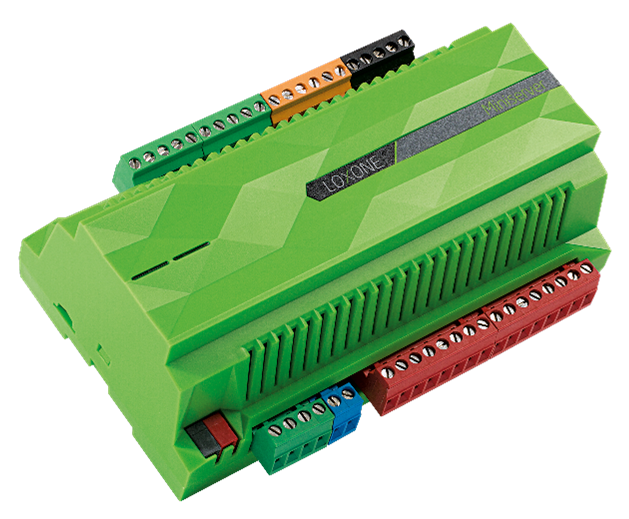
\includegraphics{obrazky/loxone-miniserver.png}
	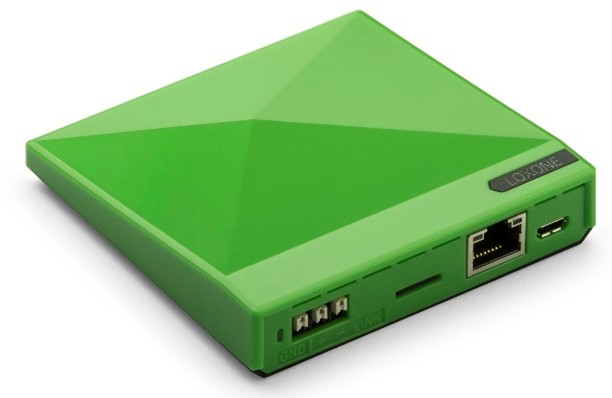
\includegraphics{obrazky/loxone-miniserver-go.jpg}
	\caption{Loxone Miniserver gen. 1 a Miniserver Go. Převzato z Loxone web}
	\label{miniserver}
\end{figure}


Všechny verze Miniserveru v sobě obsahují Loxone OS s integrovaný webový server, jsou konfigurovatelné z programu Loxone Config a ovladatelné přes mobilní aplikaci (Loxone App) [33]. Všechny miniservery obsahují slot pro SD kartu (s firmwarem). 

\begin{figure}[hbt]
	\centering
	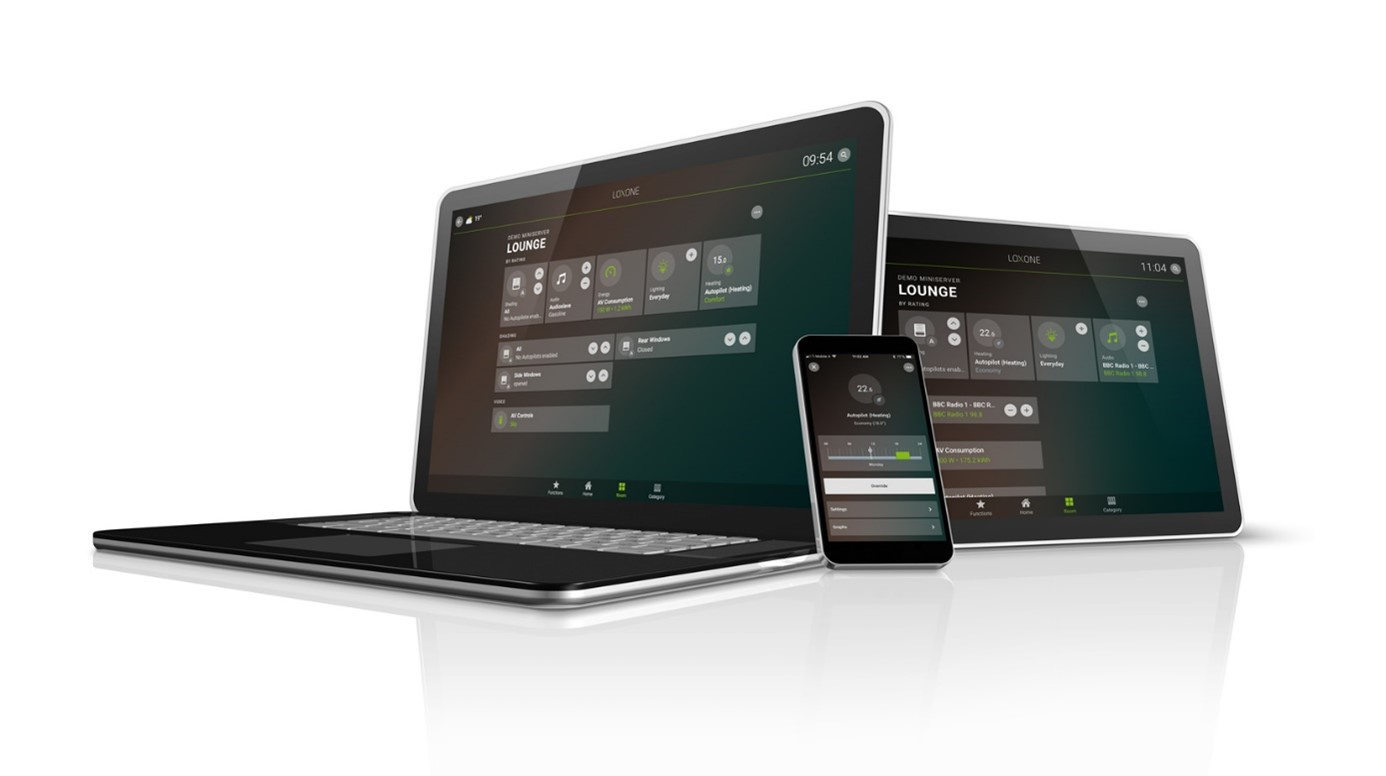
\includegraphics{obrazky/loxone-app.jpg}
	\caption{Loxone App. Převzato z Loxone web}
	\label{loxone-app}
\end{figure}

Loxone Extensions (rozšíření) slouží pro rozšíření funkcí Miniserveru. K Miniserveru se připojují pomocí sběrnice Loxone Link (kterou obsahují všechny verze Miniserveru). Tato sběrnice může být až 500 m dlouhá. Díky rozšířením může uživatel zakoupit systém pouze s těmi technologiemi, které chce opravdu využívat a nemusí tak platit za zbytečné vlastnosti systému. Příkladem rozšíření mohou být Tree Extension (pro připojení až 100 Tree zařízení; zejména pro doplnění Miniserveru 1. generace, který neobsahuje rozhraní pro komunikaci přes tree sběrnici) [36], Air Base Extension (Pro doplnění Miniserverů 1. a 2. gen – k bezdrátové komunikaci) [37], Dimmer Extension (pro stmívání světel) [38] a mnoho dalších.\newline
Loxone nabízí pro automatizaci domácnosti více než 400 produktů [33].
Loxone pro propojení prvků v systému vyvinulo tzv. Loxone Tree technologii. Jedná se o sběrnici, na kterou je možné připojit až 50 prvků, a Loxone uvádí, že díky tomu je možné ušetřit až 80\% kabeláže [DOLOŽIT!]. Podobně jako Loxone Link, i Loxone Tree může sahat až 500 m daleko. \newline

V oblasti inteligentního vytápění nabízí Loxone souhru technologií pro vytápění, chlazení, rekuperaci, a automatizovanou stínící techniku, což přináší do regulace vytápění vysokou efektivitu [34]. \newline
Z hlediska regulace teploty nabízí tzv. „zónové“ vytápění. Jedná se o inteligentní topení, které na rozdíl od klasického inteligentního vytápění (zahrnující obvykle nějaký bezdrátový termostat, wifi termostatické hlavice apod.) umožňuje inteligentněji řídit teplotu – tím že uživatel zvolí, ve které místnosti (případně i ve který čas) má být jaká teplota. Uživatel chytrého domu s tímto systémem si tak může navolit například větší teplo v koupelně oproti například místnosti kde spí. Tento systém tak umožňuje mít větší kontrolu nad vytápěnými místnostmi, potažmo vyšší efektivitu. \newline
Inteligentní vytápění Loxone podporuje režim učení, systém se tedy na základě předchozích zkušeností spustí vytápění tak, aby byla v dané místnosti požadovaná teplota ve správný čas. Uživatel si tak může nastavit například to, aby měl v 7:00 vyhřátou koupelnu na 23 °C. \newline
Loxone vytápění má dle oficiálních stránek [25] následující výhodné vlastnosti:
\begin{itemize}
    \item Inteligentní řízení teploty – využití již zmíněného režimu učení k dosažení požadované teploty v žádaný čas. Loxone rovněž při regulaci zohledňuje venkovní teplotu.
    \item Úspora nákladů – Loxone dokáže inteligentně rozhodovat o nejefektivnějším řešení. Například energeticky náročnou klimatizaci může nahradit energeticky výhodnějším stínění
    \item Režim nepřítomnosti – Systém od loxone podporuje úsporný režim pro chvíle, kdy uživatel není doma
    \item Ochrana budovy – Loxone dokáže reagovat na různá nebezpečí, například v případně vzniku požáru vypnout ventilaci i rekuperaci
    \item Loxone aplikace a statistiky – Loxone nabízí zdarma aplikaci na zařízení s androidem přes které uživatel může sledovat i nastavovat teplotu v domě vzdáleně
    \item Notifikace – V případě problému s některou technologií Loxone upozorní uživatele
    \item Státní svátky – Na základě znalosti státních svátků může Loxone adekvátně upravovat svoji činnost
    \item Údržba – Loxone uživatele upozorňuje na termín pravidelné údržby
\end{itemize}
Z hlediska automatizace domácnosti v porovnání s dříve uvedenými systémy je rovněž důležitá přítomnost ovládané chytré zásuvky. Ta s Miniserverem komunikuje technologií Loxone Air. Má v sobě teplotní čidlo a rovněž elektroměr s vyhodnocením výkonu a spotřeby \newline
//ještě zmínit loxone touch a tlačítko na stul \newline

\subsection*{Jablotron}
Jablotron je česká firma, která se od svého založení zaměřuje především na zabezpečovací systémy [40]. Kromě nich se také zabývá zabezpečením a monitoringem vozidel, topením a ventilací, monitoringem dechu a rovněž ovládáním a automatizací domácnosti [39]. \newline
Jablotron nabízí několik různých systémů. Dva nejnovější jsou Jablotron 100 a Jablotron 100+ [40]. Primárním úkolem obou systémů je zabezpečení budov, ovšem je možné je využít i v oblasti automatizace (zejména díky programovatelným výstupům). Samotné zabezpečení je možné využít v rámci automatizace (Například automatické zapnutí světel při odkódování alarmu) [43]. \newline
Na své systémy poskytuje Jablotron při splnění podmínek až 7letou záruku [42]. \newline
Pro odjištění/zajištění systému se vždy musí provést nejprve autorizace uživatele. Systém totiž uchovává informaci o oprávnění jednotlivých uživatelů. Každému z uživatelů je možné pro účely autorizace přiřadit jeden kód (4,6 nebo 8místný) a až dva RFID čipy [44]. \newline
 Typy automatizace, které je možné v těchto systémech použít jsou:
 \begin{itemize}
     \item Zapínání a vypínání
     \item Akce v kalendáři 
     \item Automatické akce [47]
 \end{itemize}
Mezi akce, které lze automatizovat v systému Jablotron patří zejména ovládání světel, ovládání žaluzií, chytrá termoregulace (řízení vytápění a klimatizace) [48] či ovládání jiných zařízení pomocí programovatelných výstupů. \newline
Systém od Jablotronu je možné rozdělit na tyto různé části:
\begin{itemize}
    \item Ústředna
    \item Různé vstupní či výstupní prvky
    \item Aplikace MyJablotron
    \item Program J-Link
\end{itemize}
Ústředna v systémech Jablotron slouží jako centrální prvek, který shromažďuje informace ze snímačů a patřičně na ně reaguje. Komunikace mezi prvky systému a ústřednou může probíhat podobně jako u systému Loxone buď pomocí kabelů, nebo bezdrátově. Zařízení, která komunikují pomocí kabelu se zde nazývají sběrnicové [43].\newline
Mezi produkty firmy Jablotron pro automatizaci domácnosti můžeme najít například:

\begin{itemize}
    \item Záplavový detektor
    \item Snímač teploty
    \item Magnetický detektor (detekce otevření dvěří/okna)
    \item Termoelektrická hlavice
    \item Relé na DIN lištu 
    \item A další [41]
\end{itemize}

Systém Jablotron 100+ je možné ovládat celkem 4 způsoby a to:
\begin{itemize}
    \item Přístupovým modulem
    \item Mobilní aplikací pro chytré telefony (MyJABLOTRON)
    \item Webovou aplikací (rovněž MyJABLOTRON)
    \item Či klíčenkou [46]
\end{itemize}

Přístupový modul slouží pro rychlé odjištění/zajištění objektu, případně k dalším funkcím automatizace. Jablotron nabízí celkem 3 typy těchto modulů:

\begin{itemize}
    \item Čtečka RFID karet
    \item Klávesnice se čtečkou RFID karet
    \item Klávesnice s displejem a čtečkou RFID karet
\end{itemize}

Ke každému z modulů je možné připojit až 20 segmentů. Ty obsahují popisek a dvě prosvětlená tlačítka. Jejich funkcí může být buďto zajištění/odjištění, signalizace stavu (například signalizace otevření garážových vrat) nebo ovládání zařízení v rámci automatizace (například žaluzií) [44]. Barvy prosvětlení odpovídají semaforu, kde červená odpovídá stavům jako zajištěno/zapnuto, žlutá zajištěno částečně a zelená znamená odjištěno/vypnuto. \newline
Jak již bylo zmíněno, systém od Jablotronu lze ovládat rovněž mobilní aplikací MyJablotron. Je k dispozici jak na Google Play (pro zařízení s androidem), tak i na App Store (pro iOS zařízení). Kromě toho existuje i její webová verze. Jablotron tak nabízí rychlý přehled o tom co se děje v domácnosti. Ovládání domácnosti přes aplikaci funguje podobným způsobem jako přístupový modul – pomocí tlačítek s barvami semaforu. \newline
Klíčenka k ovládání systému je dostupná ve dvou verzích – jednosměrný a obousměrný ovladač. Ten druhý má výhodu v tom, že provedení akce je potvrzeno kontrolkou na ovladači. V případě chyby tak ví, že je například mimo dosah ústředny a akce se neprovedla [43]. \newline
K nastavení uživatelských parametrů v systému (jako oprávnění) slouží program J-Link. V něm je možné definovat uživatele i s jejich přístupovými oprávněními, provádět diagnostiku systému, kontrolu programovatelných výstupů a vytvářet či upravovat kalendář akcí (pro ovládání automatizovaných funkcí) [47]. \newline

\subsection*{Apple HomeKit}
Apple HomeKit je systém, který umožňuje uživateli bezdrátově ovládat nejrůznější chytrá zařízení v domácnosti. Na rozdíl od systémů jako je Loxone je HomeKit určen výhradně pro bezdrátovou komunikaci. Podporuje technologie Bluetooth a Wifi. V systému tvořeném HomeKitem je potřeba nějakého centrálního prvku (hubu). Výhodou zde je, že není vždy nutné mít nějaké „mimořádné“ zařízení – jako centrální prvek zde může posloužit 


\subsection*{Sonoff}
Sonoff je bla bla…


\subsection*{homeconnect}

Zcela jiný přístup k chytré domácnosti přináší systém homeconnect…
\newpage

\chapter{Technologie dálkového přenosu}
Následující část je shrnutím technologií, používaných systémy automatizace domácnosti. Není encyklopedickým výkladem problematiky, ale souhrnem informací, které mají k práci bezprostřední vztah. První část se věnuje obecně technologii bezdrátového přenosu a dále následuje krátké seznámení s technologiemi Wifi, Bluetooth a ZigBee.

\section{Technologie bezdrátového přenosu}
Pro přenos dat či řídících signálů je vždy potřeba zvolit vhodné médium, přes které se budou tyto informace přenášet. V některých situacích není pro přenos vhodné (a někdy dokonce ani možné) používat kabely (ať už metalické nebo optické). V těchto případech je potřeba přenášet informace bezdrátově, tj. za využití jiných médií, jako je vzduch. 
Podobně jako je nutné u kabelového spojení využít vhodný způsob komunikace (například zvolit vhodnou sběrnici a nastavit ji správné parametry) je potřeba se způsobem komunikace zabývat rovněž u bezdrátového přenosu. Zde je nutné zejména zvolit vhodnou technologii (jako je Wifi, Bluetooth či ZigBee) a její parametry [A].

\subsection*{Výhody bezdrátového přenosu}
Bezdrátová komunikace má oproti kabelové řadu výhod. Zejména se jedná o následující:

\begin{itemize}
    \item Jednodušší připojení – zařízení není potřeba připojovat kabelem, a dokonce nemusí být ani vybaveno konektorem pro toto připojení (pozn. pro dálkový přenos prostřednictvím světla je však stále potřeba mít nějaký přijímající port). Z toho rovněž plyne, že není potřeba měnit strukturu sítě kvůli změnám v místnosti a rovněž není potřeba myslet na konkrétní strukturu sítě ještě před budováním.
    \item Větší spolehlivost – Častým zdrojem problémů s kabelovým připojením jsou chyby na straně kabelů – jejich poškození. Použitím bezdrátových technologií se lze vyhnout tomuto typu chyb.
    \item Snadná rozšiřitelnost sítě – U kabelového připojení je potřeba řešit způsob rozšíření sítě a v případě, že stávající struktura sítě rozšíření nepodporuje, tak je potřeba ji celou pozměnit. Bezdrátové sítě tento problém eliminují.
    \item Nižší cena – Použitím bezdrátových technologií se značně sníží pořizovací cena sítě – není potřeba kupovat drahou kabeláž. Rovněž instalace kabelů do starých budov může být velmi nákladná a problémová.
\end{itemize}

\subsection*{Nevýhody bezdrátového přenosu}
Kromě množství výhod, které bezdrátová komunikace představuje jsou zde rovněž některé nevýhody tohoto typu komunikace:

\begin{itemize}
    \item Rušení signálu – zařízení, využívající bezdrátové technologie může způsobovat rušení ostatních zařízení a rovněž opačně – dané zařízení může být rušeno od ostatních zařízení, pracujících na podobném principu
    \item Bezpečnost – bezdrátová komunikace často vysílá (a přijímá) signály do relativně rozsáhlého otevřeného prostoru, tudíž jsou takto vysílaná data často daleko méně chráněná než u kabelového přenosu (kde je k získávání dat potřeba mít fyzické připojení k síti, ve které se data přenáší) [A] [Q, str. 5-6] [R, str. 406]. Je tedy nutné zabezpečit přenos dat.
\end{itemize}


\subsection*{Způsob komunikace}
V případě bezdrátových technologií se využívá některého pásma elektromagnetického vlnění. Rychlost šíření tohoto záření je ve vakuu rovno konstantě c (přibližně 3 x 108), v médiu jako je vzduch se pak šíří rychlostí c, podělenou indexem lomu (konkrétně pro vzduch je tento index blízký 1, takže můžeme uvažovat prakticky stejnou rychlost jako pro vakuum) [M] [N, str 2-3] [O, str.24] [P, kap 8.2].\newline
V současnosti se na trhu s elektronikou zařízení, využívající především dva různé principy dálkového přenosu informací, první je založen na využití světla, druhý pak využívá rádiové vlny. [A]

\subsection*{Přenos informací pomocí světelného signálu}
V případě světelného signálu se většinou využívá infračerveného záření, jelikož není lidským okem viditelné, avšak je možné vyrobit přijímač, která tento signál detekuje (a to je vlastnost, která se zde vyžaduje). \newline
Kromě těchto definovaných protokolů je pro komunikaci pomocí IR záření možno použít standardů IEEE 802.11 (Tyto standardy to tak definují). V praxi se však nikdy nic takového nedočkalo rozšíření. \newline
První princip, který je možný použít je využití infračerveného záření. Jelikož není obvykle v domácnosti mnoho zařízení, pracujících s IR, nebývají většinou zařízení navzájem příliš rušeny. Stále zde však existuje rušení od jiných zdrojů infračerveného záření, například ze slunečního záření, nebo fluorescenčního světla. Rušení od těchto zdrojů je však možné potlačit jistými principy. Prvním je vyhrazení určité vlnové délky, která se bude pro přenos informací používat a následným použitím filtru na přijímací diodě, který odfiltruje ostatní vlnové délky. Nepotlačené rušení (od zdrojů, které vyzařují v oné vyhrazené vlnové délce (problémem je tedy zejména Slunce) je možné dále potlačit tím, že bude přijímač reagovat pouze na nějakou modulovanou frekvenci, nepřítomnou v daném zdroji (tedy například ve slunečním záření). Systémy využívající IR záření se vyznačují tím, že je musejí splňovat podmínku přímé viditelnosti vysílače a přijímače. Není tedy možné (bez případných dodatečných, opakovacích zařízení) ovládat zařízení za rohem, pokud není přímo viditelné. Právě díky této vlastnosti je možné volně využívat zařízení, využívající tohoto principu, protože nedochází k žádnému rušení a není tak potřeba regulovat směrnicemi používaní IR vysílání. Dosah IR vysílačů se obvykle udává v jednotkách, případně desítkách metrů.

\subsection*{Přenos informací pomocí rádiových vln}
Kromě IR záření mohou zařízení k dálkovému přenosu informací využívat také rádiových vln na různých frekvencích. Zde však již existují jistá omezení. Rádiové vlny se totiž (na rozdíl od IR světla) šíří i skrze předměty. To je příčinou toho, že se mohou i relativně vzdálená zařízení komunikující na stejných vlnách vzájemně rušit. Aby se předešlo naprostému zarušení prostoru, je potřeba mít k vysílání na určitých frekvencích licenci. Je zřejmé, že si běžní uživatelé zařízení v domácnosti nemohou dovolit kupovat drahé licence kvůli každému bezdrátově ovládanému zařízení, které si koupí. Z tohoto důvodu bylo navrženo tzv. pásmo ISM. \newline
V pásmu ISM jsou definovány frekvenční rozsahy, které je možné volně použít pro schválená zařízení bez licence. To ovšem také znamená, že zařízení pracující v těchto rozsazích musejí tolerovat rušení od ostatních zařízeních pracujících na stejných frekvencích. [C, s.66]. Dokument „ITU Radio Regulations“ toto pásmo vyhrazuje pro „Provoz vybavení nebo zařízení určených ke generování a využívání lokální vysokofrekvenční energie pro průmyslové, vědecké, lékařské, domácí nebo podobné účely, s výjimkou aplikací v oblasti telekomunikací“. \newline
Nejčastěji se pro komunikaci v pásmu ISM používá frekvenční pásmo 2,4 GHz. To je dané historickým vývojem. Zejména u mikrovlnných trub bylo potřeba zvolit vhodné pásmo [X]. Zvolené pásmo 2,4 Ghz bylo vybráno z několika důvodů, zejména [Everything2\_4GHZ] však na základě empirického měření průniku a šíření tepla pro různé potraviny (při použití frekvencí tohoto pásma) a s ohledem na rozměry použitého magnetronu (součástky, která generuje mikrovlnné záření [W, kap. 6-20]).

\section{Přenos pomocí WiFi}

Wifi je technologie, využívající standardů z rodiny IEEE 802.11. První verze tohoto standardu byla organizací IEEE schválena v roce 1977 [A, s.6]. Od té doby vyšlo mnoho dalších verzí standardů. Jednotlivé verze se od sebe mohou odlišovat různými parametry, například frekvenčním pásmem, šířkou pásma jednotlivých kanálů, maximální rychlostí přenosu atd. Organizace Wi-Fi Alliance rozlišuje některé standardy IEEE 802.11 číslem generace WiFi, nejnovější je prozatím zatím 6. generace (založená na standardu 802.11ax). 

\begin{figure}[hbt]
	\centering
	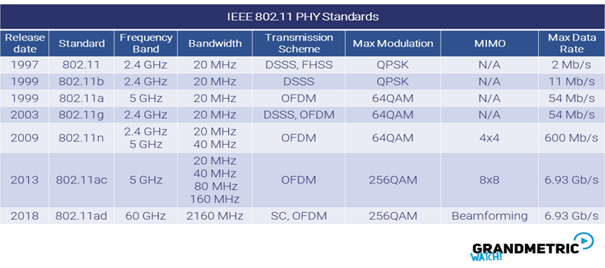
\includegraphics{obrazky/wifi-standards.png}
	\caption{Některé důležité verze standardu IEEE 802.11 a jejich parametry. Převzato z \url{https://www.grandmetric.com/2018/05/29/wi-fi-standards-evolution/}}
	\label{wifi-standards}
\end{figure}
Wifi funguje na principu vysílání a přijímání rádiových vln. Organizace IEEE rozhodla využít pro technologii Wi-Fi frekvence z pásma ISM [B, str.2]. Wifi standardně využívá frekvencí 2,4Ghz a 5Ghz. Nejprve byla zařízení Wi-Fi schopná pracovat pouze v jednom z těchto dvou frekvenčních pásem, ale 4. generace (IEEE 802.11n) přidává možnost práce v obou zmíněných pásmech. Moderní zařízení s wifi si tak mohou vybrat (a dokonce během své činnosti měnit) frekvenci, na které budou spolu komunikovat.
Obě pásma mají svá pro i proti. Mezi výhody pásma 2.4Ghz patří zejména větší pokrytí signálu a rovněž větší kompatibilita (platí spíše pro starší zařízení). Na druhou stranu pásmo 5Ghz nabízí podstatně vyšší přenosové rychlosti a dále větší množství komunikačních kanálů [D].

\subsection*{Režim sítě}
Wifi nachází uplatnění v (bezdrátových) lokálních sítích. V nich pak rozlišujeme 3 režimy na základě toho, jak se Wifi zařízení v síti mezi sebou navzájem spojují (jakou plní roli):
\begin{itemize}
    \item Režim infrastruktury
    \item Ad hoc režim
    \item Smíšený režim
\end{itemize}
V režimu infrastruktury je v sítí přítomen minimálně jeden centrální prvek (tzv. přístupový bod), který zprostředkovává komunikaci mezi jednotlivými prvky (klienty) sítě, případně poskytuje připojení do jiné sítě přes distribuční systém (DS). V tomto režimu sítě je výhoda, že je snadné připojit do stávající infrastruktury nový prvek. \newline
Ad hoc je režim bezdrátové sítě, ve které není přítomen žádný centrální prvek (přístupový bod) se kterým by prvky sítě komunikovali, ani zde není žádné spojení se pevnou sítí přes distribuční systém. Jedná se tedy o decentralizovanou síť. Jednotlivé prvky tedy mezi sebou navzájem komunikují přímo (toto spojení se někdy označuje jako tzv. peer-to-peer). V tomto režimu má síť rovněž SSID identifikátor, kterým je možné síť identifikovat. [A][B] \newline

\subsection*{Bezpečnost v síti Wi-Fi}
\todo{Todo...}
\section{Bezdrátový přenos pomocí Bluetooth}
Bluetooth je standard, definovaný v IEEE 802.15.1. Vytvořila jej firma Ericsson v roce 1994 a od té doby vyšlo několik nových verzí [A]. Podobně jako WiFi pracuje v ISM pásmu 2,4 GHz. Na rozdíl od Wi-Fi však není definován pouze na prvních dvou vrstvách ISO/OSI, ale definuje protokoly na všech sedmi vrstvách tohoto modelu. Na nejnižší úrovni, kde definuje způsob přenosu jednotlivých bitů využívá metodu FHSS, která zajišťuje, že při přenosu bitů vysílač přeskakuje mezi několika frekvencemi [AD].\newline
Zařízením, které jej využívají, umožňuje vytvořit tzv. PAN (osobní síť). V těchto sítích má každé zařízení přiřazeno unikátní 48bitovou adresu BD\_ADDR (BlueTooth Device Address) – jedná se o obdobu MAC adresy u ethernetu. Tu používá pro komunikaci s ostatními zařízeními. Jedno zařízení může být v roli master (řídící), slave (podřízená) nebo obojího [AB, str.4]. K jedné řídící stanici se připojuje jedno a více podřízených zařízení (používá se pouze adhoc komunikace mezi master a slave stanicí). Zde hovoříme o tzv. piconetu (pikosíti). Maximální počet zařízení v jedné pikosíti je 8 (jedna řídící stanice a až 7 podřízených). Stanice náležící do jedné pikosítě může zároveň patřit do jiné pikosítě. Jedná se tedy o rozšíření sítě mezi zařízeními. Takto vytvořenou síť nazýváme tzv. scatternet (rozprostřená síť). V každé rozprostřené síti má každá pikosíť unikátní identifikátor – je jím BD\_ADDR její řídící stanice. Díky rozlišení jednotlivých pikosítí pak může každá tato síť využívat jiné skokové sekvence (frekvenčních kanálů na kterých se vysílají/přijímají data) [AC, str. 20].

\section{Technologie ZigBee}
Zigbee je bezdrátová technologie, založená na standardu IEEE 802.15.4. Je určená pro vytváření sítě PAN (osobní síť) a pracuje v pásmu ISM 868 MHz, 902-928 MHz a 2,4 GHz [A]. 

\subsection*{Zařízení v ZigBee síti}
ZigBee standard specifikuje 2 typy zařízení – FFL (Full Function Device) a RFD (Reduced Function Device). FFL zařízení je obvykle schopné mnoha funkcí a je stále aktivní, zatímco RFD se nachází většinu času v režimu spánku, ze kterého se občas probudí, například aby odeslalo hodnoty neměřené na nějakém senzoru.\newline
V síti pak každé ze zařízení plní některou ze 3 funkcí:

\begin{itemize}
    \item Koordinátor
    \item Koncové zařízení
    \item Směrovač
\end{itemize}

\subsection*{Topologie sítě}
Na základě definovaných zařízení pak existují 3 možné topologie ZigBee sítě:

\begin{itemize}
    \item Hvězda
    \item Strom
    \item Mesh síť [AG, str.5]
\end{itemize}

\subsection*{ZigBee Model}
ZigBee podobně jako Bluetooth definuje komunikaci na všech úrovních modelu ISO/OSI, nekopíruje však přesně jednotlivé vrstvy. První 3 vrstvy modelů ISO/OSI a ZigBee si odpovídají, ale vrstvy L4-L7 jsou spojené do vrstev APS (Application Support) a ZDO (ZigBee Device Object). [AH, str. 42]\newline

Thread, WeMo, ZigBee and Z-Wave (https://www.tomsguide.com/us/smart-home-wireless-network-primer,news-21085.html)

\chapter{Vestavné systémy a vývojové prostředky}
\label{vestavne-systemy}
Následující část je shrnutím současného stavu v oblasti vestavných systémů a Python knihoven pro vývoj GUI aplikací. Není encyklopedickým výkladem problematiky, ale souhrnem informací, které mají k práci bezprostřední vztah. Nejprve je zde úvod do vestavných systému, následně je pojednáno o platformě Raspberry Pi, modulech ESP8266 a ESP32 a nakonec o možnostech programování GUI pomocí Python knihoven.

\section{Vestavný systém}

Vestavný systém můžeme definovat jako software spolu s počítačem, zabudovaným do nějakého zařízení takovým způsobem, že jej uživatel nevidí jako počítač [E, str.3]. Tento počítač je většinou jednoúčelový, určený pro předem navržené použití. Tím se liší od univerzálních počítačů, které mohou poskytovat různé funkce a jejichž uplatnění se může měnit (například osobní počítač) [F, str. 3].

\todo{Definovat mikropočítač, jednodeskový počítač, mikrokontrolér, mikroprocesor... (možná kapitola něco jako základní pojmy u vestavných systémů??}
\todo{Zkusit něco vytvořit z nějakého takového souhrnu: https://www.guru99.com/embedded-systems-tutorial.html}
\todo{https://jayconsystems.com/blog/microprocessor-vs-microcontroller-vs-microcomputer}
\todo{Historie smazána, vrátit ji? (Ale upravit!)}


\subsection*{Architektura řídícího zařízení}

Při návrhu systému se využívá jedna ze dvou architektur:

\begin{itemize}
    \item Von Neumannova architektura
    \item Harvardská architektura
\end{itemize}

Hlavním rozdílem je způsob práce s pamětí. Ve Von Neumannově architektuře je paměť pro program i data spojená do jedné paměti, v Harvardské architektuře je pak rozdělena. \newline
Mikroprocesor (CPU) je programovatelné elektronické výpočetní zařízení, určené pro všestranné použití. Jedná se o čip, obsahující 3 základní součásti:
\begin{itemize}
    \item Aritmeticko-logickou jednotku
    \item Řídící jednotku
    \item Registry [I, str. 18–19]
\end{itemize}

Mikroprocesor sám o sobě je z hlediska vestavěných systémů relativně jednoduché zařízení, které pro funkci systému potřebuje připojit některé další součásti, jako jsou paměti (RAM a ROM), čítače, časovač a podobně. Návrhář tedy musí tyto součásti přidat externě, aby zařízení fungovalo správně. Systémy, zahrnující mikroprocesory jsou obvykle založeny na Von Neumannově architektuře [J].\newline
Mikrokontrolér je zařízení, které na rozdíl od mikroprocesoru má již všechny součásti, potřebné pro svoji činnost v sobě. Obvykle využívá Harvardské architektury [J]. 

\section{Jednodeskový počítač Raspberry Pi}
Zařízení Raspberry Pi je levný univerzální počítač malých rozměrů. Poskytuje široké možnosti v oblasti multimédií a 3D grafiky, předpokládá se, že bude časem využíván i jako herní platforma.\newline
Název Raspberry Pi vytvořila komise dozorčí rady. Slovo Raspberry je vzato jako název ovoce (malina), jak už je u počítačových systémů zvykem nazývat podle ovoce. Slovo “Pi” označuje zkráceně “Python” - programovací jazyk, který měl být původně jediným programovacím jazykem dostupným na platformě Raspberry Pi [AA].

\subsection*{Historie}
Raspberry Pi vzniklo v r. 2006 za přispění studijního ředitele pro informatiku na Cambridgeské univerzitě za účelem lokálních potřeb. Měl to být nástroj, který by poskytl prvotní impuls studentů k nějakému z univerzitních kurzů.

\section{Moduly ESP8266 a ESP32}
Jedná se o levný mikročip, disponující Wi-Fi stackem, schopný provozu RTOS (realtime operačního systému). Je založen na 32bitovém procesoru s architekturou RISC [AE]. \newline
ESP32 je nástupce ESP8266. Kromě komunikace přes Wi-Fi umožňuje rovněž komunikaci pomocí Bluetooth, díky hybridnímu Wi-Fi/Bluetooth čipu [AF]. 


\begin{figure}[hbt]
	\centering
	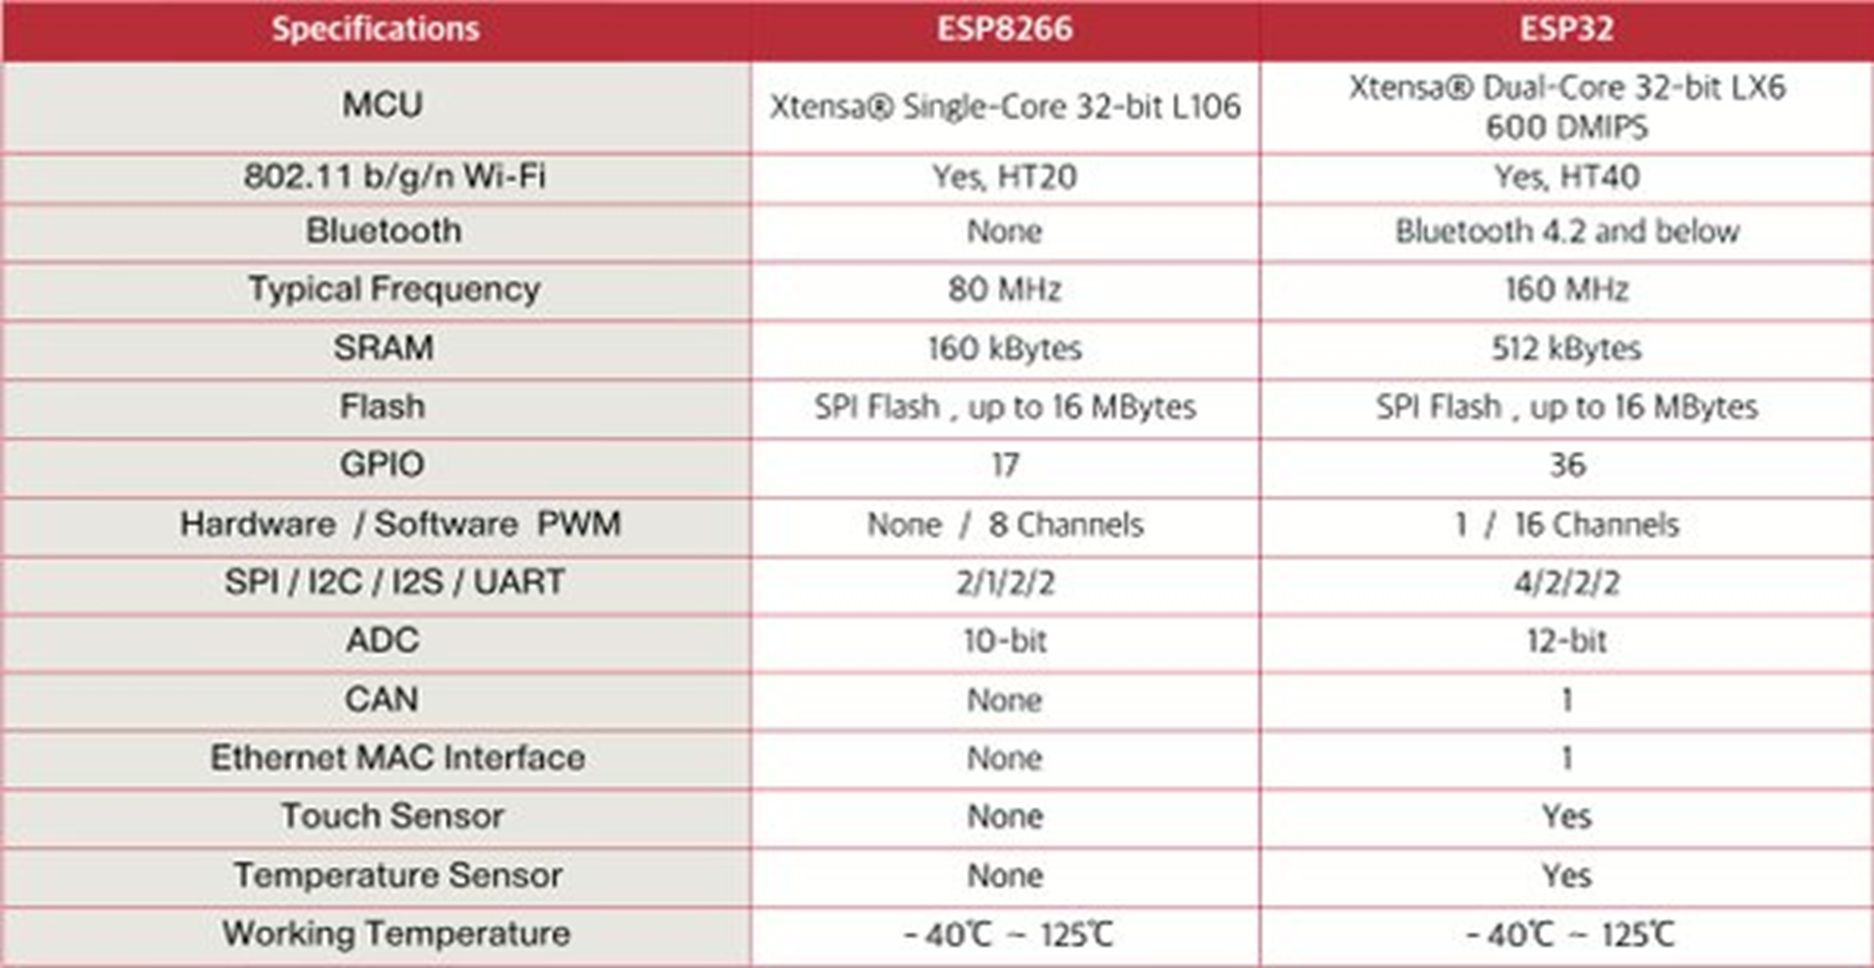
\includegraphics{obrazky/ESP.png}
	\caption{Srovnání specifikace modulů ESP8266 a ESP32. Převzato z \url{https://www.cnx-software.com/2016/03/25/esp8266-and-esp32-differences-in-one-single-table/}}
	\label{wifi-standards}
\end{figure}

\section{Python knihovny pro vývoj GUI}
K programování grafického uživatelského rozhraní existuje mnoho různých knihoven. Pro jazyk Python se nejčastěji používá některá z následujících knihoven:

\subsection*{Tkinter}

Knihovna tkinter je základní knihovna pro tvorbu okenních aplikací. Na rozdíl od ostatních knihoven je již obsažená v samotném jazyce Python, nemusí se tedy dodatečně instalovat [AL]. Používaní knihovny je tedy zdarma.\newline
Doporučuje se zvláště začátečníkům pro svou jednoduchost. Pro plnohodnotné využití je možné ke knihovně stáhnout dodatečné moduly [AM].

\subsection*{Kivy}

Knihovna Kivy patří mezi multiplatformní knihovny. Dle oficiálních stránek knihovny je možné vytvářet aplikace běžící na následujících zařízeních:

\begin{itemize}
    \item Desktopové počítače: OS X, Linux a Windows
    \item IOS zařízení: IPad a IPhone
    \item Android zařízení: tablety a telefony
    \item Jakékoli jiné dotykové zařízení, podporující TUIO (Tangible User Interface Objects) [AJ]
\end{itemize}

Knihovna přináší mnoho různých aspektů, které dle autorů knihovny mají zjednodušit tvorbu grafického rozhraní, obsluhu událostí a podobně.\newline
Ke knihovně rovněž patří zvláštní jazyk (nazvaný stejným jménem jako knihovna – jazyk Kivy). Jedním z jeho cílů je oddělení zodpovědnosti za prezentaci (zobrazení) a logiku programu [AK]. Zobrazení je dáno právě souborem kv (napsaném v jazyce Kivy) a logika souborem s Python kódem.\newline
Podobně jako tkinter, je i tato knihovna nabízena zdarma. Musí se však na rozdíl od tkinteru instalovat dodatečně.

\chapter{Zhodnocení současného stavu a plán práce}
V této kapitole se věnuji zhodnocení již existujících řešení automatizace domácnosti. Následně uvádím můj návrh řešení na základě nastudovaných řešení a vhodného rozsahu práce. Nakonec v bodech stanovuji cíle vyplývající z návrhu řešení, které se v práci snažím splnit.
\section{Současný stav}

Na trhu se v současné době nachází velké množství systémů. Z těch, které jsem popsal v části o existujících řešení je nejrozvinutějším systémem ten od společnosti Loxone. Zabírá opravdu širokou škálu možností a jen stěží by se hledala aplikace, pro kterou by nebyl vhodný. Kromě komplexnosti u něj oceňuji rovněž českou jazykovou lokalizaci. V češtině je k dispozici jak aplikace na ovládání (Loxone App), tak rovněž program pro konfiguraci systému (Loxone Config). Čím mě Loxone mile překvapilo je, že jsem si jejich aplikaci Loxone App mohl vyzkoušet v demoverzi i bez zakoupených komponent.\newline
Jako nevýhodu Loxone vidím příliš vysokou cenu. Uživatel, který si chce nainstalovat pár chytrých zařízení bude zřejmě překvapen cenou. Například při pořízení 3 chytrých zásuvek a miniserveru (který je k ovládání zásuvek potřebný) zaplatí přibližně 15 000 kč. Přitom adekvátní řešení od jiných firem, jako sonoff bude stát necelé 3000 kč, což je velký rozdíl – a při rozšiřování domácnosti o další prvky tento rozdíl znatelně roste. Na druhou stranu, pokud uživatel staví nový dům, může řešení od Loxone stát srovnatelnou cenu, jako konkurenční „neinteligentní“ instalace. Jako další nevýhodu vidím to, že celkově je instalace systému orientovaná spíše pro profesionální montáž pro pracovníky s příslušnou klasifikací (většina produktů je určena k zabudování do rozvaděče, příp. ke komunikaci s moduly v něm). Celkově je však řešení od Loxone na hodně vysoké úrovni.\newline

Řešení od firmy Jablotron je jistě zajímavé jejich dvoutlačítkovými (rozšiřitelnými) segmenty. Zdá se mi však nepraktické spojovat přístupovou klávesnici do domu s prvky automatizace domácnosti. Působí to poněkud omezeně. Navíc rozhraní pro ovládání domácnosti a alarmu v aplikaci MyJablotron se snaží napodobovat onu klávesnici, což příliš k přehlednosti nepřispívá. Na druhou stranu pro uživatele, jehož hlavní požadavek je zabezpečení objektu a pouze doplňková automatizace domácnosti (jako rozsvícení světel při odjištění domu) budou systémy od firmy Jablotron ideální.  \newline

Systém HomeKit je zajímavý v tom, že zde není potřeba žádný „speciální“ centrální prvek – pokud již uživatel vlastní například iPhone (či jiný produkt, který zastoupí funkci centrálního prvku). Nevýhodou je to, že aby byl systém ovladatelný globálně, tak je potřeba přeci jen mít v domácnosti nějaký prvek, co bude domácnost řídit. A pokud uživatel již nějaký nevlastní, tak se stává další investicí. Co je na systému HomeKit pozitivní je jeho nízká cena – ve srovnání se systémy od společnosti Loxone či Jablotron. Systém HomeKit se stále rozrůstá a má velkou podporu v rozmanitosti produktů. A na rozdíl od předchozích zmíněných systémů je více orientovaný na běžné uživatele. Jednou z nevýhod je zde to, že je systém orientovaný zejména na bezdrátovou komunikace, která samozřejmě někdy může být méně spolehlivá. Tím spíše že mnoho produktů komunikuje pouze pomocí Bluetooth, takže si uživatelé musejí hlídat dosah zařízení.\newline

Systém HomeConnect vnáší do automatizace domácnosti zajímavý koncept. Zatímco některé systémy umožňuji automatizovat domácnosti například chytrými zásuvkami či spínači, HomeConnect ve spolupráci s jinými společnostmi vyvíjí přímo spotřebiče s prvky chytré domácnosti, čímž tyto spotřebiče obsahují mnohem více „inteligence“, na rozdíl od pouhého „zapínání/vypínání“. Nicméně nevýhodou je zde příliš malý sortiment produktů, a tudíž jednoúčelová aplikace navíc, kterou stejně musejí uživatelé doplnit o další aplikace, chtějí-li například rovněž ovládat zásuvky, světla či rolety. Kromě toho je rovněž cena produktů dost vysoká.\newline
...

\section{Návrh řešení}
Na základě výzkumu dostupných řešení a jejich zhodnocení jsem se rozhodl vyvinout systém, který bude mít některé spíše základní funkce automatizace. Především zde bude řešeno dálkové ovládání jednoho zařízení druhým, jelikož je to zadání mé bakalářské práce. V systému tedy bude figurovat nějaký ovladač a dále ovládané prvky. 

V práci tudíž bude nutné zvolit vhodné vestavné zařízení, které bude sloužit jako ovládací část systému a také zařízení, která budou přijímat povely. Rozhodl jsem se, že ovládaný prvek zde nebude žádné konkrétní zařízení (jako zásuvka, spínač, či lampička) ale spíše nějaký obecný modul se vstupně výstupními porty, přes které bude možné ovládat jiná, už konkrétnější zařízení. Pro plnohodnotnou funkci systému bude tento modul nutné opatřit dalšími přídavnými součástkami. Půjde zejména o relé pro možnost ovládání zapnutí a vypnutí zařízení připojeného k tomuto modulu (tímto způsobem bude možné například ovládat LED pásek, či vytvořit bezdrátovou zásuvku). K modulu budou připojeny rovněž tranzistory pro možnost použití PWM modulace na výstupu - takový výstup pak bude sloužit pro stmívání světel, zejména LED pásku či bodových LED světel na 12 V. Ovládat tak bude možné rovněž servo motory, které se řídí PWM signálem.

Aby bylo ovládání systému co nejjednodušší, bude zde možnost ovládání na dotykovém displeji. Jelikož systém ovládaný jen z jednoho místa není v oblasti automatizace úplně nejšťastnějším a efektivním řešením (například uživatel sice nemusí dojít k vypínači světla, aby shasnul, ale stejně musí dojít někam k ovládacímu zařízení systému), rozhodl jsem se, že bude možnost ovládání i z telefonu, počítače a dalších zařízení (požadavky na zařízení budou definovaná později v části 6.X Návrh systému) \todo{Zmínit v implementaci požadavky}. Aby byl plněji využit potenciál displejů (ať už připojeného k ovládacímu zařízení, či ostatním zařízením, ze kterých bude možné moduly ovládat), rozhodl jsem se, že v systému bude možnost využívat několika různých senzorů.

Půjde o tyto senzory:
\begin{itemize}
    \item teploty
    \item pohybu
    \item sepnutí (kontaktu/tlačítka)
\end{itemize}
\todo{Uvést že dále budu ovládacímu zařízení říkat centrální prvek? Hub??}
Jde o typické představitele analogových i digitálních senzorů. Pro účely práce budou použity jen tyto tři, nicméně řešení chci pojmout jako open source (a s ohledem na tento fakt se budu snažit o co největší rozšiřitelnost systému), a další senzory bude možné přidat v budoucnu. Všechny senzory budou mít v systému pouze informativní charakter pro uživatele, tzn. bude si moci například zobrazit teplotu v konkrétní místnosti, zda se v ní někdo nachází, či zda byl sepnut nějaký kontakt (např. dveře). Nebude možné přímo systém pomocí senzorů ovládat, ale opět nic nebrání tomu, aby byla tato funkce implementována v budoucnu. U modulů s výhodou využiji, že budou mít více vstupů/výstupů a jeden modul tak může sdružovat více různých funkcí (například mít připojené 2 různé senzory a ovládat 5 výstupů).

Mým řešením bych chtěl doplnit existující open source řešení o takové, které bude svými vlastnostmi určeno spíše pro kutily v oblasti automatizace domácnosti. Bude poskytovat jednoduchý systém pro ovládání mnoha zařízení pomocí jednoho vestavného zařízení s připojeným displejem. Svou prací bych si chtěl rovněž vyzkoušet celý návrh a realizaci systému automatizace domácnosti, který bych následně mohl sám využívat. Vylepšením oproti některým již existujícím systémům bude možnost sdružení několika přijímajících zařízení do jednoho (jak jsem zmínil v předchozím odstavci).

Při práci budu využívat již existující moduly a mikropočítač (který bude sloužit jako „mozek“ systému), které však naprogramuji a vhodným způsobem doplním o některé elektronické součástky (jako zmíněné relé, či tranzistor). Práce se však nebude zabývat konstrukčním návrhem prvků systému, ani návrhem DPS pro hotový systém. Pro případně spojení komponent systému budou použita nepájivá kontaktní pole.

\section{Cíle práce}
Na základě předchozích úvah jsem se rozhodl, že vytvořím systém, který bude splňovat následující vlastnosti:

\begin{itemize}
    \item Bude zvolen vhodný mikropočítač, který bude sloužit jako ovládací část systému
    \item Pro ovládací část bude zvolen dotykový displej patřičných rozměrů, aby byl systém přehledný a mohl sloužit pro ovládání zařízení
    \item Displej by měl být rovněž vybrát s ohledem na možnost zobrazení přehledu o stavu zařízení v systému (například. zobrazení, které zařízení jsou zapnutá, či jaké hodnoty se nacházejí na PWM výstupu)
    \item K implementaci bude zvolen vhodný programovací jazyk
    \item Bude podporována funkce přímého ovládání výstupů ovládaných modulů
    \item Také zde bude funkce zobrazení dat ze senzorů
    \item Systém bude obsahovat českou jazykovou lokalizaci
    \item K systému bude možné přistupovat jak lokálně, tak i vzdáleně
    \item Pro vzdálený přístup zde budou fungovat uživatelské účty, přičemž z jednoho účtu bude možné ovládat jen jednu domácnost
    \item Bude zvolena vhodná technologie bezdrátového přenosu tak, aby byl systém co nejjednodušší na implementaci a případné rozšiřování
    \item Projekt bude uvolněn jako open source, čímž bude cena systému jako takového pro potenciální uživatele minimální (daná pouze cenou použitých součástek a zařízení)
\end{itemize}

\chapter{Realizace a testování}
V této kapitole se věnuji vlastní realizaci řešení a následnému testování a vyhodnocení. V první podkapitole uvádím celkový návrh systému -tedy z jakých aplikací a zařízení se bude skládat, jak mezi sebou budou komunikovat apod. Následně se věnuji návrhu grafického uživatelského rozhraní pro aplikaci, ke kterým uživatel bude přistupovat. V dalších kapitolách již rozebírám implementaci konkrétních aplikací. Nakonec uvádím jak jsem systém testoval a k jakým výsledkům testy vedly.
\todo{Někde vymezit pojmy...klient, klientská aplikace, (koncový) modul...}
\section{Celkový návrh systému}
Systém se bude skládat celkem ze tří aplikací a několika zařízení (každé zde bude mít svou roli). 

\subsection*{Zařízení}
Jmenovitě budou v systému fungovat tato zařízení:
\begin{itemize}
    \item Centrální jednotka (s připojeným displejem)
    \item Koncové moduly
    \item Senzory
    \item Ovládaná zařízení
    \item Ostatní zařízení, přes která bude možné systém ovládat (klienti)
\end{itemize}

Centrální jednotka bude mít na starosti celý systém řídit. Pokud například uživatel zadá pokyn ke změně hodnoty na některém výstupu modulu, bude to právě Centrální jednotka, kdo tuto žádost (v jistém smyslu) přijme a pošle ji dále jako příkaz na konkrétní koncový modul.
Jelikož k centrální jednotce bude potřeba připojit (dotykový) displej, musí mít dostatečný výkon pro vykreslování na něj a zpracování dat. Bylo tedy potřeba zvolit vhodný mikropočítač (protože mikrokontrolery mívají obecně daleko menší výkon) opatřený nějakým portem pro přenos obrazu. Jedním z nejpoužívanějším a také nejrychleji vyvíjejícím se mikropočítačem je Raspberry Pi, vlastní ho tedy již mnoho IT\todo{?} nadšenců. Je relativně levné (ve verzi 3 se dá sehnat do jednoho tisíce kč, verzi Zero W je dokonce možné na českém trhu sehnat za přibližně 300 kč) a tedy i snadno dostupné. Nadto je použití Raspberry Pi doporučeno v zadání mé práce.

Koncový modul (dále již jen modul) bude zařízení, které bude mít nějaké vstupy a výstupy. Modul bude měnit hodnoty na svých výstupech dle instrukcí, přicházejících z centrální jednotky. K těmto výstupů pak budou dále připojeny příslušné součástky (jako relé, či tranzistor) a k nim dále již reálná zařízení, ve kterých budou nějakým způsobem spínat kontakt. Rovněž bude v pravidelných intervalech číst hodnoty na svých vstupech (ke kterým budou připojeny senzory). Jako koncový modul je potřeba vybrat zařízení s nízkou cenou, jelikož těchto zařízení může být i více. Kromě toho bude modul přijímat pouze jednoduché příkazy od Raspberry Pi, může se tedy klidně jednat o nějaký mikrokontroler s omezeným výpočetním výkonem. Je však potřeba, aby byl tento mikrokontroler schopný komunikovat po síti (tento požadavek vyplývá ze zadání mé bakalářské práce). Na trhu existují především 2 takové mikrokontrolery - ESP8266 a novější ESP32.

Ovládanými zařízeními zde myslím ta, co budou připojena na některý z výstupů modulu. Půjde tedy například o LED pásek, či zařízení, u kterého bude spínat kontakt.

Klientská zařízení budou libovolná zařízení, přes které bude uživatel moci ovládat systém. Jedinými požadavky na tato zařízení jsou zde vzhledem k implementaci:
\begin{itemize}
    \item Přístup k internetu
    \item Dostatečně velký displej (ideálně 5´´ a více)
\end{itemize}

\subsection*{Aplikace}
Dále kromě zařízení budou v systému fungovat tyto tři aplikace:
\begin{itemize}
    \item Klientská aplikace (dále již jen klient), určená jako grafické rozhraní pro uživatele k ovládání systému
    \item Server, který bude od klienta (ať už přímo, nebo zprostředkovaně skrze databázi) získávat instrukce a vykonávat je
    \item Aplikace na modulech
\end{itemize}

Po úvaze jsem dospěl k názoru, že nejvhodnější bude, když bude klient implementován jako jednostránková webová aplikace. A to z několika důvodů:
\begin{itemize}
    \item Webové aplikace jsou obecně vzato multiplatformní (pokud mají alespoň trochu responzivní design), čehož vhodně využiji v rámci možnosti ovládat domácnost i na dálku
    \item K přístupu k aplikaci tak bude stačit mít zařízení s přístupem k internetu (a obrazovkou pochopitelně)
    \item Webové technologie patří mezi rychle se rozvíjející, což přispívá k budoucímu rozvoji systému
    \item Jazyk Typescript (který budu používat) je jeden z vůbec nejpoužívanějších a nejznámějších programovacích jazyků, pokud se tedy najde programátor, který by chtěl v budoucnu systém rozšířit, je velká pravděpodobnost se nebude muset učit nic nového.
\end{itemize}

\begin{figure}[!hbt]
	\centering
	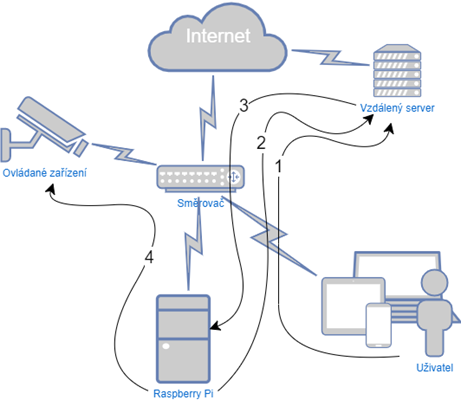
\includegraphics[scale=0.7]{obrazky/architektura.png}
	\caption{Architektura systému pro automatizaci domácnosti}
	\label{architektura}
\end{figure}
\todo{Upravit scale obrázku výše!}

Druhá aplikace pak bude běžet na Raspberry Pi jako server zpracující požadavky jednak od klientů, a pak také samozřejmě požadavky zadané přímo na displeji Raspberry Pi \todo{...rozvést...}


Jako alternativu těchto prvních dvou aplikací bylo možné vytvořit jen jednu, běžící na Raspberry Pi, přes kterou by se systém ovládal pouze z připojeného displeje. Nicméně tímto by se ztratila možnost ovládat systém i vzdáleně, resp. i z jiných zařízení, než je Raspberry Pi, což by bylo jistě neintuitivní a mnohdy nepříjemné, zvolil jsem tedy řešení dvou aplikací.

\subsection*{Programové prostředky}
\todo{Vysvětlit proč jsem si vybral zrovna typescript a node.js a jaké jsou alternativy (a alternativní řešení)}

\subsection*{Celková architektura systému}
\todo{Uvést celkově co s čím a jak bude komunikovat, dle obrázku \ref{architektura} (a vytvořit nový)}

Na obrázku \ref{architektura} je možné vidět celkovou koncepci systému.


\section{Grafický návrh klientské aplikace}
Aplikace byla rozdělena na několik samostatných částí (oken), mezi kterými může uživatel přecházet. Jelikož se jedná o jedno stránkovou aplikaci, nejde v případě jednotlivých částí o klasické stránky (v tom smyslu, že by každá měla vlastní html dokument, který ji generuje). V následujícím textu se však budu odkazovat ke každému takovému samostatnému oknu, jako k jedné (webové) stránce.
\subsection*{Přihlašovací stránka a registrace}
Na úvod při spuštění se zobrazí stránka, na které se uživatel bude moci přihlásit (pomocí emailu a hesla). Rovněž zde bude možnost přejít k registraci nového účtu, vyžádat si zapomenuté heslo či projít dále do aplikace bez přihlášení (tato možnost bude pouze v aplikaci Raspberry Pi).

\subsection*{Menu}
V aplikaci se přihlášenému uživateli bude zobrazovat vyjíždějící menu, kterým se bude moci přepínat mezi jednotlivými stránkami (jako domovská stránka či nastavení). V menu také bude možnost odhlášení, která však pravděpodobně nebude často využívána.
\subsection*{Domovská stránka}
Za domovskou stránku považuji tu, na kterou se uživatel dostane ihned po přihlášení do systému. Tato stránka bude sloužit i jako výchozí pro ovládání jednotlivých zařízení. Bude zde také přehled hodnot na senzorech. Tuto stránku bude mít uživatel zobrazenou většinu času na displeji Raspberry Pi, pokud jej bude chtít používat jako takový rychlý přehled o stavech ovládaných zařízení (a senzorech).
Jak vidíme na obrázku XYm bude tato stránka rozvržena na jednotlivé místnosti. Pro každou zde bude pod sebou vyhrazené místo a v něm pro každou místnost se stejným rozvržením - název místnosti, seznam hodnot na senzorech a ovládaná zařízení (ze kterých bude možné vyčíst jejich stav i ovládat je). Pokud bude chtít uživatel ovládat nějaké zařízení, klikne na něj. V případě zařízení typu zapnuto/vypnuto se okamžitě změní stav zařízení. V případě zařízení, řízených PWM modulací se zobrazí nad zařízeními posuvník (nastavený na aktuální hodnotu), kterým bude možné okamžitě měnit hodnotu na výstupu modulu (a tedy stav zařízení).

\subsection*{Nastavení}
V aplikaci bude také stránka s nastavením. Bude zde možnost přidávat nová zařízení a konfigurovat ta stávající...
\todo{Dodělat...Nebude zde nastavení a konfigurace zvlášť?}


\section{Implementace klientské aplikace}
\todo{Zmínit že spárování uživ. účtu s RPi bude tím, že se přihlásí uživatel na lokálním serveru}
\section{Implementace serveru na Raspberri Pi}
\section{Implementace aplikace pro koncové moduly}
\section{Testování a vyhodnocení systému}


\subsection*{Provedené testy}
V rámci testování jsem provedl tyto testy:
\begin{itemize}
    \item Test reaktivity
    \item Test intuitivnosti uživatelského prostředí
    \item Test stability při potížemi s připojením k internetu
    \item Test autonomie?
\end{itemize}

Test reaktivity (neboli odezvy systému na podněty v reálném čase) probíhal takto...

Test intuitivnosti uživatelského prostředí probíhal takto...

Test Test stability při potížemi s připojením k internetu probíhal takto...

Test autonomie (funkce systému bez lidského zásahu) probíhal takto...

\subsection*{Testy které nebyli provedeny}
Kromě testů, které jsem už provedl by bylo vhodné provést ještě dále zmíněné. V případě absence prvních dvou nedojde k žádným potížím (jen systém možná nebude fungovat na jiných zařízeních). Problémy, které by se otestovali zbylými dvěma testy by však mohli být kritické. Alespoň u čtvrtého testu ale věřím, že nejsou obavy na místě, přeci jen je konkurence velká a systém by neměl být zahlcený. V rámci mé práce tyto testy vykonány nebyli, zejména z finančních a časových důvodů.
Testy které by bylo vhodné provést:
\begin{itemize}
    \item Funkčnost systému na alternativních mikropočítačích 
    \item Funkčnost systému na jiných verzích Raspberry Pi
    \item Stabilita systému v průběhu několika let chodu
    \item Test spolehlivosti systému při velkém množství uživatelů
\end{itemize}
Raspberry Pi je jedním z nejpoužívanějších a nejznámějších mikroprocesorů, nicméně na trhu se nacházejí další, u kterých by bylo vhodné otestovat, zda bude server i klientská aplikace (na připojeném displeji) plně funkční. Zejména mikropočítače uvedené v kapitole \ref{vestavne-systemy} (tam jsem totiž popisoval rovněž nejpopulárnější mikropočítače)

Funkčnost systému na jiných verzích Raspberry Pi je potřeba otestovat zejména z toho důvodu, že se jedná o poměrně rychle se rozvíjející platformu a někteří potenciální uživatelé tak mohou mít starší model s nižším výkonem. Zvláště zajímavý by byl test na verzi Zero W, jelikož tuto verzi Raspberry Pi je možné pořídit za přibližně 300 kč. V případě bezproblémového chodu by byl projekt velmi zajímavou alternativou k některým velmi drahým systémům jako je \todo{XYZ}. Je možné, že by například nebyla tato verze Raspberry Pi dostatečně výkoná na ovládání systému z připojeného displeje, ale zvládala by na běh aplikace serveru, pak by bylo možné systém prostě ovládat z klientů (například chytrých telefonů). Případně kdyby tato verze nezvládala bezproblémový běh serveru s poskytováním statické stránky, tak by bylo možné tuto část serveru upravit (odstranit) a pak by se klienti připojovali pouze na vzdálený server a úloha Raspberry Pi by se zredukovala pouze na kontrolu (resp. naslouchání) změn v databázi a komunikaci s koncovými moduly, což by snad mělo opravdu bez jakýchkoli potíží fungovat. Pak by se samozřejmě muselo vyřešit spárování Raspberry Pi s uživatelským účtem, protože aktuálně to funguje právě na principu, který vyžaduje, aby se uživatel (alespoň poprvé) přihlásil na poskytované statické stránce z Raspberry Pi.

Test stability systému by pak spočíval v tom, že by systém pravidelně po dobu několika let využívalo jisté množství lidí (například 100 domácností) a pozorovalo, zda se systém v průběhu času chová stále stejně, nezpomaluje se a podobně.

Test spolehlivosti systému při velkém množství uživatelů by bylo provést hlavně z toho důvodu, že v systému funguje jedna veřejná databáze. Vylo by vhodné otestovat, jak se systém bude chovat při velké zátěži databáze (ve chvíli, kdy bude k databázi aktivně současně přistupovat mnoho uživatelů).






























\chapter{Závěr}
\label{zaver}

Nápady na pokračování práce:
\begin{itemize}
    \item ovládání hlasem
    \item přidání podmínek
    \item přidání módů (scén) - v podstatě by se jednalo o sdružení více akcí ovládání do jedné
    \item vývoj by mohl směřovat i na odlehčení serveru tak, že bude pouze kontrolovat databázi a komunikovat s moduly (jak bylo polemizováno v testování) => a mohla by se vytvořit verze pro ESP8266 v režimu Centrální jednotky => velice levný systém...
\end{itemize}

Moje odkazy \cite{4technologie} \cite{BezdratoveSite} \cite{DesigningEmbeddedSystems} \cite{EmbeddedSystems}
\cite{EmbeddedSystemsCircuits}
\cite{ITURegulations} \cite{MicroprocessorAndInterfaces} \cite{WifiFrequencyBands} \cite{uCvsCPU} \cite{arduino} \cite{ArduinoProgramming} \cite{whatIsIR} \cite{optics} \cite{physics} \cite{HomeAutomationRPI} \cite{Everything2_4GHZ} \cite{microwave} \cite{materials} \cite{wirelessComunication} \cite{NetworkSecurity} \cite{RPiPrirucka} \cite{BluetoothGuide} \cite{WirelessPersonalCommunications} \cite{GettingStartedBluetooth} \cite{Why2_4GHz} \cite{ESP8266} \cite{ESP32} \cite{HandsOnZigBee} \cite{ZigbeeWirelessNetworking}


%===============================================================================

  %% Tento soubor nahraďte vlastním souborem s přílohami (nadpisy níže jsou pouze pro příklad)

% Umístění obsahu paměťového média do příloh je vhodné konzultovat s vedoucím
%\chapter{Obsah přiloženého paměťového média}

%\chapter{Manuál}

%\chapter{Konfigurační soubor}

%\chapter{RelaxNG Schéma konfiguračního souboru}

%\chapter{Plakát}

  
  
  \ifenglish
    %\input{projekt-01-kapitoly-chapters-en}
  \else
    %% Tento soubor nahraďte vlastním souborem s obsahem práce.
%=========================================================================
% Autoři: Michal Bidlo, Bohuslav Křena, Jaroslav Dytrych, Petr Veigend a Adam Herout 2019
\chapter{Úvod}
Zde bude cca jedna strana úvod…

\blindtext[2]
\todo{Upravit}.


\chapter{Automatizace domácnosti}
Následující část je shrnutím současného stavu v oblasti automatizace domácnosti a chytrých domovů. Není encyklopedickým výkladem problematiky, ale souhrnem informací, které mají k práci bezprostřední vztah. Nejprve je zde popis automatizace domácnosti, co to je, jaké jsou dnes možnosti jejího využití, přínosy a používané principy.

\section{Automatizace domácnosti a chytrý dům}
Automatizace domácnosti spočívá v automatizování činností, které řídí domácnost, normálně vykonávané člověkem. Můžeme ji definovat jako mechanismus, který nahrazuje lidskou námahu (při ovládání domácnosti), natolik, nakolik je to jen možné [U]. V souvislosti s tím někdy hovoříme o inteligentní, řízené či chytré domácnosti. Jedná se o kolekci zařízení a (pod)systémů, které jsou schopny spolu komunikovat či fungovat nezávisle. Přitom automatizovaný „dům budoucnosti“ slibují výrobci domácích zařízení prakticky již téměř od počátku minulého století [1]. Chytrý dům (či smart home) je pak definován jako dům, vybavený výpočetní a informační technologií, které předvídá uživatelovi potřeby a odpovídá na ně, a přitom dbá na jeho pohodlí, bezpečnost a zábavu [13]. Často se tedy tyto dva pojmy (automatizovaný a chytrý dům) zaměňují, ačkoli \todo{Z nějakého nového zdroje rozvést, viz odkaz}
\begin{verbatim}
https://www.google.com/search?q=smart+home+vs+home+automation&rlz=1C1AVFC_enCZ780CZ780&oq=smart+home+vs+hom&aqs=chrome.0.0i19j69i57j0i19i22i30j0i5i13i19i30l5.7375j0j7&sourceid=chrome&ie=UTF-8
\end{verbatim}




\subsection*{Možnosti využití automatizace v domácnosti}
Automatizace v mnohém usnadňuje život a umožňuje provádění akcí, které by jinak byli prakticky nemožné (například zabezpečení domu, efektivní řízení vytápění domácnosti a spotřeby energie). V současné době patří automatizace domácnosti mezi rychle se rozvíjející technologie \todo{Dopsat zdroj, viz  odkaz} []. 
\begin{verbatim}
https://www.google.com/search?q=home+automation+is+fast+developing&rlz=1C1AVFC_enCZ780CZ780&oq=home+automation+is+fast+deveopin&aqs=chrome.1.69i57j33i10i160.14343j0j7&sourceid=chrome&ie=UTF-8
\end{verbatim} 
Mezi typické aplikace automatizace domácnosti patří například:
\begin{itemize}
\item Zabezpečovací systém
\item Systém pro inteligentní vytápění a ventilaci (HVAC)
\item Zábava a multimédia
\item Komunikace
\item Osvětlení [3]
\item Ovládání spotřebičů [T]
\item Samo zavlažovací systémy [U]
\item A mnoho dalšího
\end{itemize}

\begin{figure}[hbt]
	\centering
	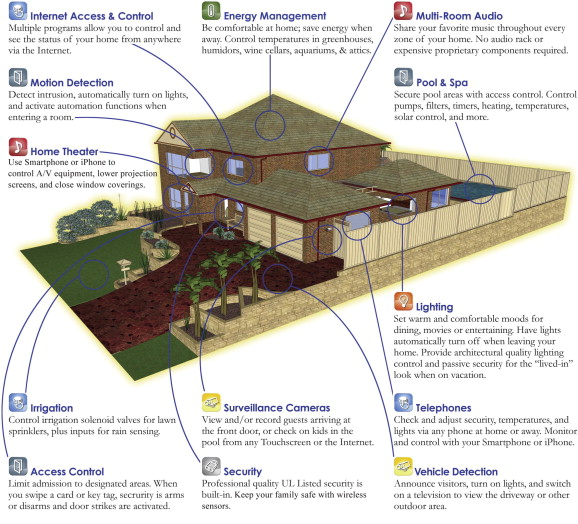
\includegraphics{obrazky/automation-example.jpg}
	\caption{Příklad možností automatizované domácnosti[U]}
	\label{asd}
\end{figure}
Nejaky text, mozna spise az sem o tom, že "V současné době patří automatizace domácnosti mezi rychle se rozvíjející technologie".


\newpage
\subsection*{Přínosy automatizace domácnosti}
Přidání inteligence do domácnosti přináší do života lidí řadu přínosů. Jde zejména o:

\begin{itemize}
\item Bezpečí – Chytré domy mohou používat různé senzory, které detekují nebezpečí a v souvislostí s nimi provést patřičné akce k jejich zabránění, případně minimalizaci škod. Příkladem mohou být záplavové a kouřové senzory a v neposlední řadě také zabezpečovací systém domácnosti.
\item Komfort – Chytré domácnosti svými funkcemi nabízejí různé způsoby, jak jejich uživatelům zpříjemnit různé rutinní akce. Mohou se postarat o automatické nastavování žaluzií dle intenzity venkovního světla, přes dotykový displej na dálku ztlumit světlo či hlasovým pokynem uvést celý byt do jiného světelného režimu. 
\item Přehled o provozu – Systémy pro automatizaci domácnosti zahrnují i displeje s přehledem o stavu jednotlivých zařízení a čidel. Také je v některých systémech možné tyto informace sledovat i z chytrých telefonů, tabletů či počítačů (a to i vzdáleně). V některých komplexnějších systémech, které například zahrnují komunikaci přes mobilní sítě je možné získávat přehled o provozu dokonce pomocí SMS zprávy (hodí se třeba při absenci internetového připojení) [15]
\item Úspora – V chytrých domácnostech je možné použít inteligentní vytápění domu založené na údajích z teplotních čidel, denní doby, případně nastaveném režimu domácnosti. Společnost ELKO EP odhaduje, že díky bezdrátové regulaci topení je možné ušetřit až 30 \% nákladů na energii [17]. Úsporu rovněž zajistí automatizovaná světla, o kterých je možné mít v automatizované domácnosti vždy přehled, na dálku je zapínat/vypínat dle potřeby a rovněž je napojit na senzory, které je budou ovládat například na základě přítomnosti osob v místnosti.
\end{itemize}
    

\subsection*{Základní klasifikace chytré domácnosti}
Chytrou domácnost můžeme rozdělit dle kabeláže:

\begin{itemize}
\item Drátovou
\item Bezdrátovou 
\item Kombinovanou
\end{itemize}
Pokud má být domácnost komplexně automatizovaná, je často vhodnější mít celý systém propojený pomocí kabelů, jelikož takový systém bude spolehlivější a v případě potřeby nabízí rychlejší přenos dat (například pokud mají být součástí systému multimédia). Bezdrátové systémy se hodí zejména tam, kde není žádané zasahovat do elektroinstalace, či pokud uživatel potřebuje pouze jednodušší systém (například s ovládáním několika málo zařízení). Připravená kabeláž pro automatizaci domácnosti rovněž přináší výhodu snadnějšího řešení napájení jednotlivých chytrých zařízení, které se tak může rozvádět po bytě spolu s datovými kabely. Přitom pro propojení jednotlivých chytrých zařízení mezi sebou je možné využít různé typy kabelů (např. ethernetový) [15]. Systémy s kombinovanou kabeláží pak vycházejí z klasické kabelové instalace s možností použití některých bezdrátových prvků (např. snímačů).


\subsection*{Mechanismy používané v chytrých domovech}
V chytrém domě se při automatizaci obvykle používají následující principy:

\begin{itemize}
\item Přímé ovládání spotřebičů
\item Nastavení scény
\item Podmínky [16, pokud neseženu lepší]
\end{itemize}
Přímé ovládání spotřebičů se obvykle provádí dálkovým ovládáním, používá-li spotřebič pro komunikaci technologii rádiového přenosu na frekvencích 443 MHz. Příkladem takového zařízení může být „bla bla bla“ od společnosti...Jiný způsob ovládání rovněž zahrnuje použití jiného chytrého zařízení (například chytrého telefonu), pokud ovládané zařízení umí komunikovat pomocí stejné technologie (např. WiFi). Ovládání pomocí telefonu či podobného chytrého zařízení je možné i v případě, že ovládané zařízení neumí komunikovat stejnou technologií, ale v domácnosti existuje centrální prvek (hub), který podporuje obě technologie a funguje zde jako prostředník mezi oběma zařízeními. \newline
V chytrých domovech je rovněž často možné použít rovněž nastavení některé předem definované scény. Tato scéna sdružuje několik příkazů přímého ovládání. Může se například jednat o scénu odchodu z domu, která vypne všechna světla, odpojí spotřebiče od elektrické sítě a aktivuje zabezpečovací systém.\newline
Dalším principem uplatňovaným v chytrém domě jsou nastavené podmínky. Ty způsobí, že při určité akci systém zareaguje nějakým předem nastaveným způsobem. Například se může jednat o podmínku, aby v případě že s….\newline

\subsection*{Komponenty chytré domácnosti}
Na trhu dnes existuje nepřeberné množství různých systémů. Typická automatizovaná domácnost využívá některé (či všechny) z následujících komponent: \newline

\begin{itemize}
\item Vstupní prvky (různá čidla, tlačítka, dotykové displeje…)
\item Výstupní prvky (Světla, spotřebiče a různá zařízení)
\item Virtuální (hlasový) asistent
\item Centrální jednotka
\item Aplikace pro řízení domácnosti z chytrých zařízení (telefonu, tabletu, počítače…)
\end{itemize}

\subsection*{Chytrá zařízení a IoT}
\todo{todo}

\subsection*{Protokoly používané v automatizaci domácnosti}
\todo{todo - MQTT atd...}
\todo{Možná změnit uplně kapitolu technol. bezdrátového přenosu na Protokoly a tam radši dát MQTT atd?}


\section{Virtuální hlasoví asistenti a centrální prvky chytré domácnosti}
Virtuální osobní asistent (VPA) je osobní asistent, který zajišťuje interakci mezi uživatelem chytré domácnosti a zařízeními v ní. Jako jiné označení se rovněž používá inteligentní či digitální osobní asistent, či mobilní asistent. Je-li ovládaný hlasem, pak se někdy označuje jako hlasový asistent [6]. Dále v textu této kapitoly je vždy asistentem míněn právě hlasový asistent, nebude-li specifikováno jinak. Jedná se o software, jehož úlohou je asistovat uživateli při nejrůznějších příležitostech, mezi jinými i při ovládání domácnosti. Hlasoví asistenti běží na některém zařízení s reproduktorem a mikrofony nebo mobilním zařízení. Dnes jich existuje na trhu veliké množství (zejména pro chytré telefony), mezi jejich nejznámější představitele v současné době patří:
\begin{itemize}
\item Apple Siri
\item Amazon Alexa
\item Microsoft Cortana
\item Google Assistant [2]
\item Samsung S voice
\item Facebook M
\item Nuance dragon [6]
\end{itemize}
V současné době žádný z výše uvedených hlasových systémů nepodporuje češtinu, nicméně Assistant od společnosti Google by ji v dohledné době mohl podporovat [14]. Amazon Alexa pak sice nerozumí česky, ale již dokáže číst některé knihy v češtině []ttt. Pro českého uživatele jsou tak pouze 2 možnosti – buďto používat asistenta v angličtině a spokojit se s případnou absencí některých funkcí, které nejsou v česku podporované (UVÉST KTERÉ A CITOVAT ZDROJ – NAPŘÍKLAD VOLÁNÍ JEN V USA, BEZTAK I NAKUPOVÁNÍ???), nebo použít některého českého virtuálního asistenta, ovšem s omezenou funkcionalitou oproti jejich „něco“ protějškům. Mezi české hlasové asistenty patří například:
\begin{itemize}
\item Emma
\item Intelli
\end{itemize}
Zmínit se o českých asistentech (EMMA, INTELLI) a najít další
\ subsection*{Použití virtuálních asistentů}
Každý z virtuálních asistentů má své vlastní specifikace, ovšem jsou typy úloh, které vykonávají více méně všichni asistenti:
\begin{itemize}
\item Číst a psát SMS a emailové zprávy, uskutečňovat hovory
\item Nastavovat časové a kalendářové akce (časovače, upomínky…)
\item Odpovídat na některé základní informativní otázky (počasí, čas, převody jednotek…)
\item Ovládat média jako televizi či připojené reproduktory (pouštět filmy, hudbu)
\item Vyprávět vtipy a příběhy
\item Konečně ovládat prvky chytré domácnosti [2]
\end{itemize}
Používání virtuálních osobních asistentů nejen, že umožňuje přistupovat k různým úkolům inovativním a interaktivním způsobem, ale v mnoha případech i zjednodušuje jinak relativně zdlouhavou činnost. Dobrým příkladem je například manuální nastavení budíku (bez použití VPA). Na mobilním telefonu (Nexus 5) je potřeba vykonat následující akce:
\begin{enumerate}
\item Kliknout na tlačítko pro návrat na domovskou obrazovku (pokud se tam uživatel nenachází)
\item Kliknout na ikonu hodin
\item V otevřené aplikaci najít ikonu budíku a kliknout na ni 
\item Kliknout na tlačítko „+“ pro přidání budíku
\item Nastavit hodinu, překliknout na volbu minuty a nastavit minuty
\item Potvrdit kliknutím na tlačítko „OK“
\end{enumerate}
Při použití hlasového asistenta je celá úloha značně zredukována pouze na aktivování asistenta a vyslovení požadovaného úkolu [6]. \newline
Bez použití VPA je dokonce řada úkolů nerealizovatelná. Například připomenout či udělat něco v okamžiku, kdy se uživatel vrátí domů, což je funkce, kterou někteří virtuální asistenti podporují [16]. Interaktivitu zajišťují virtuální asistenti i při automatizaci domácnosti, pro její řízení není potřeba otevírat k tomu určené (a mnohdy jednoúčelové) aplikace, ale stačí vyslovit žádost, třeba i s jistou vzdáleností od zařízení s hlasovým asistentem a ten se již o vše postará [DOLOŽIT!!!]. Kromě toho, virtuální asistenti v sobě mohou nést i funkce sloužící přímo pro automatizaci domácnosti. Například nastavení podmínek, scénářů atd [Rozveď to a uved nejaky zdroj!!!]. \newline
Virtuální asistenti díky svým funkcím a vlastnostem k chytré domácnosti neodmyslitelně patří, ovšem je nutné si uvědomit, že zde nejsou nutností. Spíše často fungují jako prostředník mezi uživatelem a chytrými zařízeními, který usnadňuje řízení domácnosti. Často pak bývají zabudováni do chytrého zařízení, plnící funkci centrálního prvku (hubu), jako například v případě zařízení Echo od společnosti Amazon. [DOLOŽIT NĚJAK!!!] \newline
\ subsection*{Amazon}
\ subsection*{Google}
\ subsection*{Microsoft}
\ subsection*{Apple}
\ subsection*{Emma}

Emma je český hlasový asistent, kterého vytvořil David Beck pomocí aplikace Zkratky (na systému iOS). Jak již bylo zmíněno, nativním virtuálním asistentem pro iPhone je Siry, ta však neumí česky, a to se rozhodl David Beck změnit [20]. Nejedná se o samostatnou aplikaci, ale o zkratku v aplikaci Zkratky na systému iOS. Tato aplikace zkratky umožňuje uživatelům sloučit různé akce do jedné zkratky. Celkově pro zkratku Emma nastavil 7 tisíc akcí a další se chystá přidávat. Systém v současné době již podporuje češtinu, částečně slovenštinu a polštinu. Plánuje také přidat maďarštinu, řečtinu a rumunštinu [21]. 

\section{Existující řešení chytrých domů}
Dnes je na trhu nepřeberné množství systémů, lišících se v ceně, komplexnosti, způsobem komunikace a podobně. Jednou z nejčastějších aplikací automatizace, kterou různé společnosti nabízejí je ovládání světel a zásuvek. Mezi další aplikace patří ovládání hlavic radiátorů, chytré termostaty, ovládání ventilátorů, stínící techniky, alarm a podobně. Mezi konkrétní systémy, které jsou dostupné na českém trhu patří:
\begin{itemize}
\item Loxone
\item Jablotron
\item Apple HomeKit
\item Sonoff
\item Fibaro
\item Homeconnect
\item A mnoho dalších
\end{itemize}
Kromě komerčně prodávaných systémů je k dispozici rovněž open source řešení, mezi známější patří například:
\begin{itemize}
\item Home Assistant
\item A další
\end{itemize}

\subsection*{Loxone}
Loxone je společnost, zaměřující se na automatizaci budov, v rozsahu od malých bytů, přes hotely až po rozsáhlé budovy a výrobní haly. Zaměřují se na širokou škálu aplikací, v oblasti automatizace domácnosti jde zejména o:
\begin{itemize}
\item Bezpečnost (Pohybové senzory, dveřní a okenní senzory)
\item Přístup do budovy (Přístup kódem zadávaným na klávesnici, NFC přívěškem či iButtonem, kamera)
\item Řízení filtrace bazénu
\item Větrání (Automatické řízení ventilace, například na základě přítomnosti osoby, vlhkosti, teplotě…)
\item Regulace teploty (Loxone je možné připojit k jakémukoli zdroji teploty i chlazení)
\item Úspora energie (Ovládání budovy k úsporám energie – například automatické stínění jako ochrana přetopení ze slunečního tepla)
\item Osvětlení (ovládání bodového světla, LED pásků či Loxone závěsných světel)
\item Multimédia (Ovládání audia, TV…)
\item Stínění (Ovládání stínící techniky pomáhá při vytápění a chlazení v domě)
\item A díky rozšířením také mnoho dalšího [32]
\end{itemize}
Systém loxone se skládá z několika různých prvků:

\begin{itemize}
\item Miniserver
\item Rozšíření
\item Příslušenství (Loxone Tree zařízení)
\item Loxone Tree a Loxone Link kabeláž
\item Aplikace Loxone App a Loxone Config
\end{itemize}
Loxone prvky ke své činnosti potřebují tzv. miniserver. Ten v systému funguje jako centrální řídící jednotka, která se stará o automatizaci domácnosti. Loxone nabízí celkem 3 různé verze miniserveru:

\begin{itemize}
\item Miniserver Gen. 1
\item Miniserver Gen. 2
\item Miniserver Go
\end{itemize}

Miniserver 1. i 2. generace mají oba 8 digitálních a 4 analogové vstupy a 8 digitálních výstupů (relé spínající max 250VAC/30VDC). Miniserver 1. generace má ještě navíc 4 analogové výstupy [27]. Obě generace miniserveru slouží pro kabelovou komunikaci a jsou určené k instalaci na DIN lištu. Také jsou obě generace vybaveny rozhraním Loxone Link (pro kabelové připojení až 30 tzv. rozšíření) a LAN port (Fast ethernet). Pouze první generace obsahuje KNX rozhraní, naopak pouze druhá generace a verze Go obsahují již integrované rozhraní Loxone Tree (K první generaci je pro komunikaci po Loxone Tree sběrnici dodat rozšiřující modul) [28]. \newline
Pokud si uživatel přeje využívat bezdrátové komunikace mezi prvky systému Loxone (zejména Pro bezdrátové ovládání pak Loxone nabízí 3. verzi miniserveru – Miniserver Go. Ten komunikuje s bezdrátovými periferiemi (rozšířeními a příslušenstvím) rádiovou komunikací na frekvenci 868MHz pro SRD pásmo pro Evropu (na 4 kanálech), případně 915MHz pro ITU region 2 (10 kanálů), s maximálním výkonem 3.16 mW [26]. Obsahuje také LAN port (Fast ethernet) a rozhraní Loxone Link. K této verzi miniserveru je možné bezdrátově připojit až 128 periferií [31].

\begin{figure}[hbt]
	\centering
	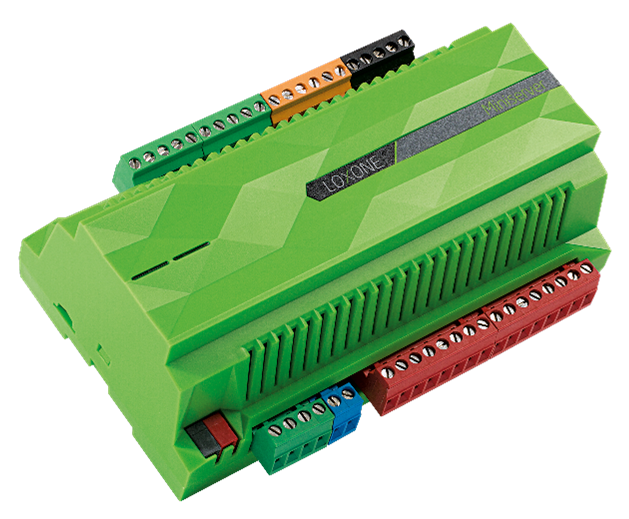
\includegraphics{obrazky/loxone-miniserver.png}
	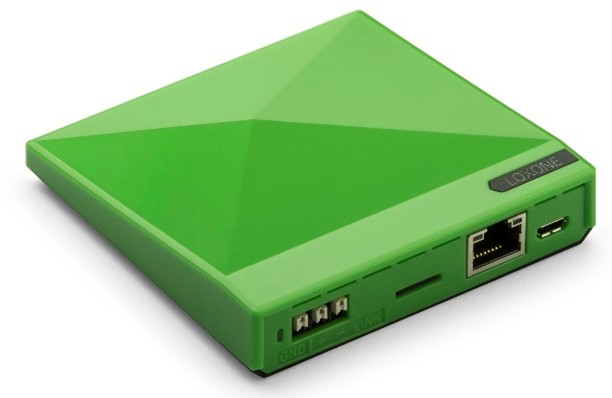
\includegraphics{obrazky/loxone-miniserver-go.jpg}
	\caption{Loxone Miniserver gen. 1 a Miniserver Go. Převzato z Loxone web}
	\label{miniserver}
\end{figure}


Všechny verze Miniserveru v sobě obsahují Loxone OS s integrovaný webový server, jsou konfigurovatelné z programu Loxone Config a ovladatelné přes mobilní aplikaci (Loxone App) [33]. Všechny miniservery obsahují slot pro SD kartu (s firmwarem). 

\begin{figure}[hbt]
	\centering
	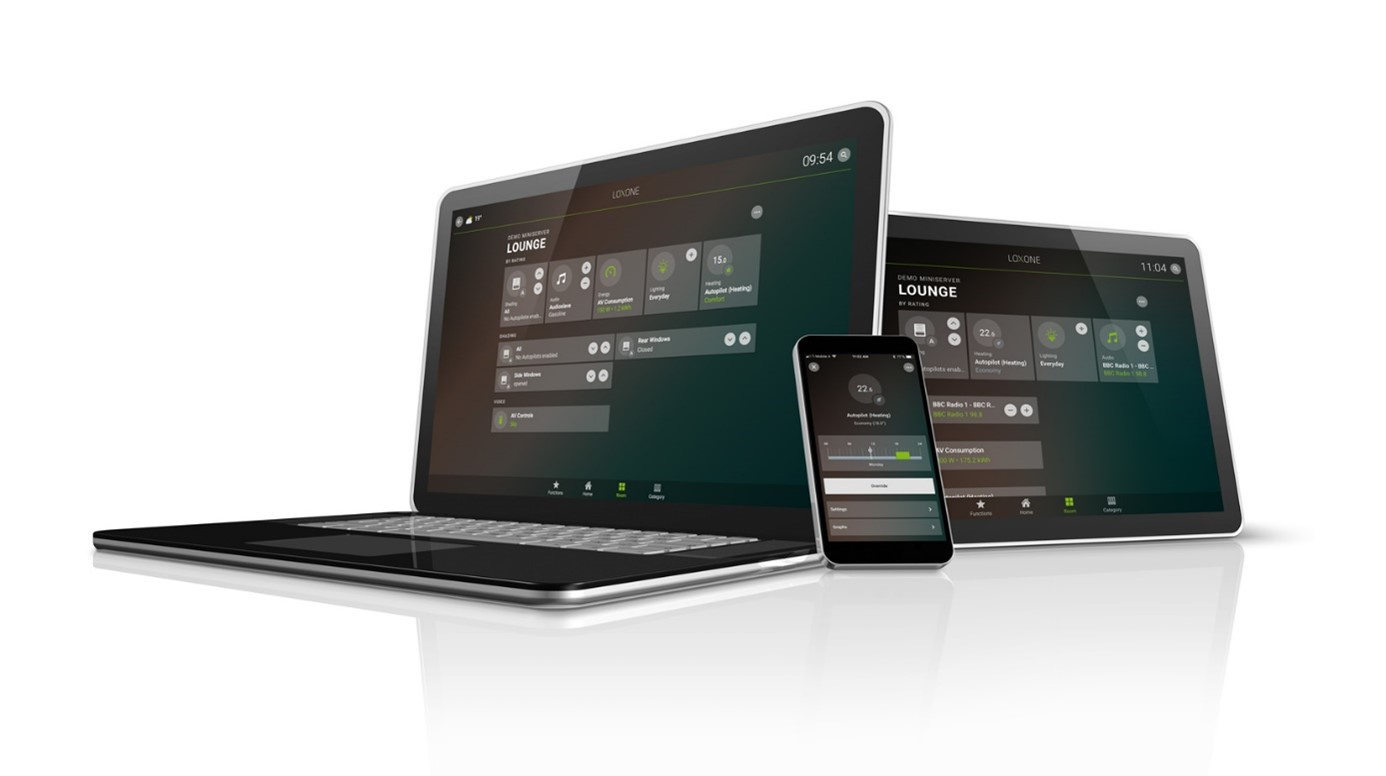
\includegraphics{obrazky/loxone-app.jpg}
	\caption{Loxone App. Převzato z Loxone web}
	\label{loxone-app}
\end{figure}

Loxone Extensions (rozšíření) slouží pro rozšíření funkcí Miniserveru. K Miniserveru se připojují pomocí sběrnice Loxone Link (kterou obsahují všechny verze Miniserveru). Tato sběrnice může být až 500 m dlouhá. Díky rozšířením může uživatel zakoupit systém pouze s těmi technologiemi, které chce opravdu využívat a nemusí tak platit za zbytečné vlastnosti systému. Příkladem rozšíření mohou být Tree Extension (pro připojení až 100 Tree zařízení; zejména pro doplnění Miniserveru 1. generace, který neobsahuje rozhraní pro komunikaci přes tree sběrnici) [36], Air Base Extension (Pro doplnění Miniserverů 1. a 2. gen – k bezdrátové komunikaci) [37], Dimmer Extension (pro stmívání světel) [38] a mnoho dalších.\newline
Loxone nabízí pro automatizaci domácnosti více než 400 produktů [33].
Loxone pro propojení prvků v systému vyvinulo tzv. Loxone Tree technologii. Jedná se o sběrnici, na kterou je možné připojit až 50 prvků, a Loxone uvádí, že díky tomu je možné ušetřit až 80\% kabeláže [DOLOŽIT!]. Podobně jako Loxone Link, i Loxone Tree může sahat až 500 m daleko. \newline

V oblasti inteligentního vytápění nabízí Loxone souhru technologií pro vytápění, chlazení, rekuperaci, a automatizovanou stínící techniku, což přináší do regulace vytápění vysokou efektivitu [34]. \newline
Z hlediska regulace teploty nabízí tzv. „zónové“ vytápění. Jedná se o inteligentní topení, které na rozdíl od klasického inteligentního vytápění (zahrnující obvykle nějaký bezdrátový termostat, wifi termostatické hlavice apod.) umožňuje inteligentněji řídit teplotu – tím že uživatel zvolí, ve které místnosti (případně i ve který čas) má být jaká teplota. Uživatel chytrého domu s tímto systémem si tak může navolit například větší teplo v koupelně oproti například místnosti kde spí. Tento systém tak umožňuje mít větší kontrolu nad vytápěnými místnostmi, potažmo vyšší efektivitu. \newline
Inteligentní vytápění Loxone podporuje režim učení, systém se tedy na základě předchozích zkušeností spustí vytápění tak, aby byla v dané místnosti požadovaná teplota ve správný čas. Uživatel si tak může nastavit například to, aby měl v 7:00 vyhřátou koupelnu na 23 °C. \newline
Loxone vytápění má dle oficiálních stránek [25] následující výhodné vlastnosti:
\begin{itemize}
    \item Inteligentní řízení teploty – využití již zmíněného režimu učení k dosažení požadované teploty v žádaný čas. Loxone rovněž při regulaci zohledňuje venkovní teplotu.
    \item Úspora nákladů – Loxone dokáže inteligentně rozhodovat o nejefektivnějším řešení. Například energeticky náročnou klimatizaci může nahradit energeticky výhodnějším stínění
    \item Režim nepřítomnosti – Systém od loxone podporuje úsporný režim pro chvíle, kdy uživatel není doma
    \item Ochrana budovy – Loxone dokáže reagovat na různá nebezpečí, například v případně vzniku požáru vypnout ventilaci i rekuperaci
    \item Loxone aplikace a statistiky – Loxone nabízí zdarma aplikaci na zařízení s androidem přes které uživatel může sledovat i nastavovat teplotu v domě vzdáleně
    \item Notifikace – V případě problému s některou technologií Loxone upozorní uživatele
    \item Státní svátky – Na základě znalosti státních svátků může Loxone adekvátně upravovat svoji činnost
    \item Údržba – Loxone uživatele upozorňuje na termín pravidelné údržby
\end{itemize}
Z hlediska automatizace domácnosti v porovnání s dříve uvedenými systémy je rovněž důležitá přítomnost ovládané chytré zásuvky. Ta s Miniserverem komunikuje technologií Loxone Air. Má v sobě teplotní čidlo a rovněž elektroměr s vyhodnocením výkonu a spotřeby \newline
//ještě zmínit loxone touch a tlačítko na stul \newline

\subsection*{Jablotron}
Jablotron je česká firma, která se od svého založení zaměřuje především na zabezpečovací systémy [40]. Kromě nich se také zabývá zabezpečením a monitoringem vozidel, topením a ventilací, monitoringem dechu a rovněž ovládáním a automatizací domácnosti [39]. \newline
Jablotron nabízí několik různých systémů. Dva nejnovější jsou Jablotron 100 a Jablotron 100+ [40]. Primárním úkolem obou systémů je zabezpečení budov, ovšem je možné je využít i v oblasti automatizace (zejména díky programovatelným výstupům). Samotné zabezpečení je možné využít v rámci automatizace (Například automatické zapnutí světel při odkódování alarmu) [43]. \newline
Na své systémy poskytuje Jablotron při splnění podmínek až 7letou záruku [42]. \newline
Pro odjištění/zajištění systému se vždy musí provést nejprve autorizace uživatele. Systém totiž uchovává informaci o oprávnění jednotlivých uživatelů. Každému z uživatelů je možné pro účely autorizace přiřadit jeden kód (4,6 nebo 8místný) a až dva RFID čipy [44]. \newline
 Typy automatizace, které je možné v těchto systémech použít jsou:
 \begin{itemize}
     \item Zapínání a vypínání
     \item Akce v kalendáři 
     \item Automatické akce [47]
 \end{itemize}
Mezi akce, které lze automatizovat v systému Jablotron patří zejména ovládání světel, ovládání žaluzií, chytrá termoregulace (řízení vytápění a klimatizace) [48] či ovládání jiných zařízení pomocí programovatelných výstupů. \newline
Systém od Jablotronu je možné rozdělit na tyto různé části:
\begin{itemize}
    \item Ústředna
    \item Různé vstupní či výstupní prvky
    \item Aplikace MyJablotron
    \item Program J-Link
\end{itemize}
Ústředna v systémech Jablotron slouží jako centrální prvek, který shromažďuje informace ze snímačů a patřičně na ně reaguje. Komunikace mezi prvky systému a ústřednou může probíhat podobně jako u systému Loxone buď pomocí kabelů, nebo bezdrátově. Zařízení, která komunikují pomocí kabelu se zde nazývají sběrnicové [43].\newline
Mezi produkty firmy Jablotron pro automatizaci domácnosti můžeme najít například:

\begin{itemize}
    \item Záplavový detektor
    \item Snímač teploty
    \item Magnetický detektor (detekce otevření dvěří/okna)
    \item Termoelektrická hlavice
    \item Relé na DIN lištu 
    \item A další [41]
\end{itemize}

Systém Jablotron 100+ je možné ovládat celkem 4 způsoby a to:
\begin{itemize}
    \item Přístupovým modulem
    \item Mobilní aplikací pro chytré telefony (MyJABLOTRON)
    \item Webovou aplikací (rovněž MyJABLOTRON)
    \item Či klíčenkou [46]
\end{itemize}

Přístupový modul slouží pro rychlé odjištění/zajištění objektu, případně k dalším funkcím automatizace. Jablotron nabízí celkem 3 typy těchto modulů:

\begin{itemize}
    \item Čtečka RFID karet
    \item Klávesnice se čtečkou RFID karet
    \item Klávesnice s displejem a čtečkou RFID karet
\end{itemize}

Ke každému z modulů je možné připojit až 20 segmentů. Ty obsahují popisek a dvě prosvětlená tlačítka. Jejich funkcí může být buďto zajištění/odjištění, signalizace stavu (například signalizace otevření garážových vrat) nebo ovládání zařízení v rámci automatizace (například žaluzií) [44]. Barvy prosvětlení odpovídají semaforu, kde červená odpovídá stavům jako zajištěno/zapnuto, žlutá zajištěno částečně a zelená znamená odjištěno/vypnuto. \newline
Jak již bylo zmíněno, systém od Jablotronu lze ovládat rovněž mobilní aplikací MyJablotron. Je k dispozici jak na Google Play (pro zařízení s androidem), tak i na App Store (pro iOS zařízení). Kromě toho existuje i její webová verze. Jablotron tak nabízí rychlý přehled o tom co se děje v domácnosti. Ovládání domácnosti přes aplikaci funguje podobným způsobem jako přístupový modul – pomocí tlačítek s barvami semaforu. \newline
Klíčenka k ovládání systému je dostupná ve dvou verzích – jednosměrný a obousměrný ovladač. Ten druhý má výhodu v tom, že provedení akce je potvrzeno kontrolkou na ovladači. V případě chyby tak ví, že je například mimo dosah ústředny a akce se neprovedla [43]. \newline
K nastavení uživatelských parametrů v systému (jako oprávnění) slouží program J-Link. V něm je možné definovat uživatele i s jejich přístupovými oprávněními, provádět diagnostiku systému, kontrolu programovatelných výstupů a vytvářet či upravovat kalendář akcí (pro ovládání automatizovaných funkcí) [47]. \newline

\subsection*{Apple HomeKit}
Apple HomeKit je systém, který umožňuje uživateli bezdrátově ovládat nejrůznější chytrá zařízení v domácnosti. Na rozdíl od systémů jako je Loxone je HomeKit určen výhradně pro bezdrátovou komunikaci. Podporuje technologie Bluetooth a Wifi. V systému tvořeném HomeKitem je potřeba nějakého centrálního prvku (hubu). Výhodou zde je, že není vždy nutné mít nějaké „mimořádné“ zařízení – jako centrální prvek zde může posloužit 


\subsection*{Sonoff}
Sonoff je bla bla…


\subsection*{homeconnect}

Zcela jiný přístup k chytré domácnosti přináší systém homeconnect…
\newpage

\chapter{Technologie dálkového přenosu}
Následující část je shrnutím technologií, používaných systémy automatizace domácnosti. Není encyklopedickým výkladem problematiky, ale souhrnem informací, které mají k práci bezprostřední vztah. První část se věnuje obecně technologii bezdrátového přenosu a dále následuje krátké seznámení s technologiemi Wifi, Bluetooth a ZigBee.

\section{Technologie bezdrátového přenosu}
Pro přenos dat či řídících signálů je vždy potřeba zvolit vhodné médium, přes které se budou tyto informace přenášet. V některých situacích není pro přenos vhodné (a někdy dokonce ani možné) používat kabely (ať už metalické nebo optické). V těchto případech je potřeba přenášet informace bezdrátově, tj. za využití jiných médií, jako je vzduch. 
Podobně jako je nutné u kabelového spojení využít vhodný způsob komunikace (například zvolit vhodnou sběrnici a nastavit ji správné parametry) je potřeba se způsobem komunikace zabývat rovněž u bezdrátového přenosu. Zde je nutné zejména zvolit vhodnou technologii (jako je Wifi, Bluetooth či ZigBee) a její parametry [A].

\subsection*{Výhody bezdrátového přenosu}
Bezdrátová komunikace má oproti kabelové řadu výhod. Zejména se jedná o následující:

\begin{itemize}
    \item Jednodušší připojení – zařízení není potřeba připojovat kabelem, a dokonce nemusí být ani vybaveno konektorem pro toto připojení (pozn. pro dálkový přenos prostřednictvím světla je však stále potřeba mít nějaký přijímající port). Z toho rovněž plyne, že není potřeba měnit strukturu sítě kvůli změnám v místnosti a rovněž není potřeba myslet na konkrétní strukturu sítě ještě před budováním.
    \item Větší spolehlivost – Častým zdrojem problémů s kabelovým připojením jsou chyby na straně kabelů – jejich poškození. Použitím bezdrátových technologií se lze vyhnout tomuto typu chyb.
    \item Snadná rozšiřitelnost sítě – U kabelového připojení je potřeba řešit způsob rozšíření sítě a v případě, že stávající struktura sítě rozšíření nepodporuje, tak je potřeba ji celou pozměnit. Bezdrátové sítě tento problém eliminují.
    \item Nižší cena – Použitím bezdrátových technologií se značně sníží pořizovací cena sítě – není potřeba kupovat drahou kabeláž. Rovněž instalace kabelů do starých budov může být velmi nákladná a problémová.
\end{itemize}

\subsection*{Nevýhody bezdrátového přenosu}
Kromě množství výhod, které bezdrátová komunikace představuje jsou zde rovněž některé nevýhody tohoto typu komunikace:

\begin{itemize}
    \item Rušení signálu – zařízení, využívající bezdrátové technologie může způsobovat rušení ostatních zařízení a rovněž opačně – dané zařízení může být rušeno od ostatních zařízení, pracujících na podobném principu
    \item Bezpečnost – bezdrátová komunikace často vysílá (a přijímá) signály do relativně rozsáhlého otevřeného prostoru, tudíž jsou takto vysílaná data často daleko méně chráněná než u kabelového přenosu (kde je k získávání dat potřeba mít fyzické připojení k síti, ve které se data přenáší) [A] [Q, str. 5-6] [R, str. 406]. Je tedy nutné zabezpečit přenos dat.
\end{itemize}


\subsection*{Způsob komunikace}
V případě bezdrátových technologií se využívá některého pásma elektromagnetického vlnění. Rychlost šíření tohoto záření je ve vakuu rovno konstantě c (přibližně 3 x 108), v médiu jako je vzduch se pak šíří rychlostí c, podělenou indexem lomu (konkrétně pro vzduch je tento index blízký 1, takže můžeme uvažovat prakticky stejnou rychlost jako pro vakuum) [M] [N, str 2-3] [O, str.24] [P, kap 8.2].\newline
V současnosti se na trhu s elektronikou zařízení, využívající především dva různé principy dálkového přenosu informací, první je založen na využití světla, druhý pak využívá rádiové vlny. [A]

\subsection*{Přenos informací pomocí světelného signálu}
V případě světelného signálu se většinou využívá infračerveného záření, jelikož není lidským okem viditelné, avšak je možné vyrobit přijímač, která tento signál detekuje (a to je vlastnost, která se zde vyžaduje). \newline
Kromě těchto definovaných protokolů je pro komunikaci pomocí IR záření možno použít standardů IEEE 802.11 (Tyto standardy to tak definují). V praxi se však nikdy nic takového nedočkalo rozšíření. \newline
První princip, který je možný použít je využití infračerveného záření. Jelikož není obvykle v domácnosti mnoho zařízení, pracujících s IR, nebývají většinou zařízení navzájem příliš rušeny. Stále zde však existuje rušení od jiných zdrojů infračerveného záření, například ze slunečního záření, nebo fluorescenčního světla. Rušení od těchto zdrojů je však možné potlačit jistými principy. Prvním je vyhrazení určité vlnové délky, která se bude pro přenos informací používat a následným použitím filtru na přijímací diodě, který odfiltruje ostatní vlnové délky. Nepotlačené rušení (od zdrojů, které vyzařují v oné vyhrazené vlnové délce (problémem je tedy zejména Slunce) je možné dále potlačit tím, že bude přijímač reagovat pouze na nějakou modulovanou frekvenci, nepřítomnou v daném zdroji (tedy například ve slunečním záření). Systémy využívající IR záření se vyznačují tím, že je musejí splňovat podmínku přímé viditelnosti vysílače a přijímače. Není tedy možné (bez případných dodatečných, opakovacích zařízení) ovládat zařízení za rohem, pokud není přímo viditelné. Právě díky této vlastnosti je možné volně využívat zařízení, využívající tohoto principu, protože nedochází k žádnému rušení a není tak potřeba regulovat směrnicemi používaní IR vysílání. Dosah IR vysílačů se obvykle udává v jednotkách, případně desítkách metrů.

\subsection*{Přenos informací pomocí rádiových vln}
Kromě IR záření mohou zařízení k dálkovému přenosu informací využívat také rádiových vln na různých frekvencích. Zde však již existují jistá omezení. Rádiové vlny se totiž (na rozdíl od IR světla) šíří i skrze předměty. To je příčinou toho, že se mohou i relativně vzdálená zařízení komunikující na stejných vlnách vzájemně rušit. Aby se předešlo naprostému zarušení prostoru, je potřeba mít k vysílání na určitých frekvencích licenci. Je zřejmé, že si běžní uživatelé zařízení v domácnosti nemohou dovolit kupovat drahé licence kvůli každému bezdrátově ovládanému zařízení, které si koupí. Z tohoto důvodu bylo navrženo tzv. pásmo ISM. \newline
V pásmu ISM jsou definovány frekvenční rozsahy, které je možné volně použít pro schválená zařízení bez licence. To ovšem také znamená, že zařízení pracující v těchto rozsazích musejí tolerovat rušení od ostatních zařízeních pracujících na stejných frekvencích. [C, s.66]. Dokument „ITU Radio Regulations“ toto pásmo vyhrazuje pro „Provoz vybavení nebo zařízení určených ke generování a využívání lokální vysokofrekvenční energie pro průmyslové, vědecké, lékařské, domácí nebo podobné účely, s výjimkou aplikací v oblasti telekomunikací“. \newline
Nejčastěji se pro komunikaci v pásmu ISM používá frekvenční pásmo 2,4 GHz. To je dané historickým vývojem. Zejména u mikrovlnných trub bylo potřeba zvolit vhodné pásmo [X]. Zvolené pásmo 2,4 Ghz bylo vybráno z několika důvodů, zejména [Everything2\_4GHZ] však na základě empirického měření průniku a šíření tepla pro různé potraviny (při použití frekvencí tohoto pásma) a s ohledem na rozměry použitého magnetronu (součástky, která generuje mikrovlnné záření [W, kap. 6-20]).

\section{Přenos pomocí WiFi}

Wifi je technologie, využívající standardů z rodiny IEEE 802.11. První verze tohoto standardu byla organizací IEEE schválena v roce 1977 [A, s.6]. Od té doby vyšlo mnoho dalších verzí standardů. Jednotlivé verze se od sebe mohou odlišovat různými parametry, například frekvenčním pásmem, šířkou pásma jednotlivých kanálů, maximální rychlostí přenosu atd. Organizace Wi-Fi Alliance rozlišuje některé standardy IEEE 802.11 číslem generace WiFi, nejnovější je prozatím zatím 6. generace (založená na standardu 802.11ax). 

\begin{figure}[hbt]
	\centering
	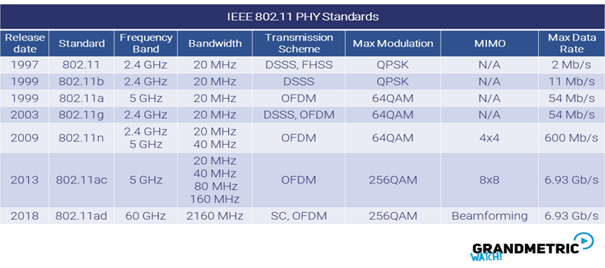
\includegraphics{obrazky/wifi-standards.png}
	\caption{Některé důležité verze standardu IEEE 802.11 a jejich parametry. Převzato z \url{https://www.grandmetric.com/2018/05/29/wi-fi-standards-evolution/}}
	\label{wifi-standards}
\end{figure}
Wifi funguje na principu vysílání a přijímání rádiových vln. Organizace IEEE rozhodla využít pro technologii Wi-Fi frekvence z pásma ISM [B, str.2]. Wifi standardně využívá frekvencí 2,4Ghz a 5Ghz. Nejprve byla zařízení Wi-Fi schopná pracovat pouze v jednom z těchto dvou frekvenčních pásem, ale 4. generace (IEEE 802.11n) přidává možnost práce v obou zmíněných pásmech. Moderní zařízení s wifi si tak mohou vybrat (a dokonce během své činnosti měnit) frekvenci, na které budou spolu komunikovat.
Obě pásma mají svá pro i proti. Mezi výhody pásma 2.4Ghz patří zejména větší pokrytí signálu a rovněž větší kompatibilita (platí spíše pro starší zařízení). Na druhou stranu pásmo 5Ghz nabízí podstatně vyšší přenosové rychlosti a dále větší množství komunikačních kanálů [D].

\subsection*{Režim sítě}
Wifi nachází uplatnění v (bezdrátových) lokálních sítích. V nich pak rozlišujeme 3 režimy na základě toho, jak se Wifi zařízení v síti mezi sebou navzájem spojují (jakou plní roli):
\begin{itemize}
    \item Režim infrastruktury
    \item Ad hoc režim
    \item Smíšený režim
\end{itemize}
V režimu infrastruktury je v sítí přítomen minimálně jeden centrální prvek (tzv. přístupový bod), který zprostředkovává komunikaci mezi jednotlivými prvky (klienty) sítě, případně poskytuje připojení do jiné sítě přes distribuční systém (DS). V tomto režimu sítě je výhoda, že je snadné připojit do stávající infrastruktury nový prvek. \newline
Ad hoc je režim bezdrátové sítě, ve které není přítomen žádný centrální prvek (přístupový bod) se kterým by prvky sítě komunikovali, ani zde není žádné spojení se pevnou sítí přes distribuční systém. Jedná se tedy o decentralizovanou síť. Jednotlivé prvky tedy mezi sebou navzájem komunikují přímo (toto spojení se někdy označuje jako tzv. peer-to-peer). V tomto režimu má síť rovněž SSID identifikátor, kterým je možné síť identifikovat. [A][B] \newline

\subsection*{Bezpečnost v síti Wi-Fi}
\todo{Todo...}
\section{Bezdrátový přenos pomocí Bluetooth}
Bluetooth je standard, definovaný v IEEE 802.15.1. Vytvořila jej firma Ericsson v roce 1994 a od té doby vyšlo několik nových verzí [A]. Podobně jako WiFi pracuje v ISM pásmu 2,4 GHz. Na rozdíl od Wi-Fi však není definován pouze na prvních dvou vrstvách ISO/OSI, ale definuje protokoly na všech sedmi vrstvách tohoto modelu. Na nejnižší úrovni, kde definuje způsob přenosu jednotlivých bitů využívá metodu FHSS, která zajišťuje, že při přenosu bitů vysílač přeskakuje mezi několika frekvencemi [AD].\newline
Zařízením, které jej využívají, umožňuje vytvořit tzv. PAN (osobní síť). V těchto sítích má každé zařízení přiřazeno unikátní 48bitovou adresu BD\_ADDR (BlueTooth Device Address) – jedná se o obdobu MAC adresy u ethernetu. Tu používá pro komunikaci s ostatními zařízeními. Jedno zařízení může být v roli master (řídící), slave (podřízená) nebo obojího [AB, str.4]. K jedné řídící stanici se připojuje jedno a více podřízených zařízení (používá se pouze adhoc komunikace mezi master a slave stanicí). Zde hovoříme o tzv. piconetu (pikosíti). Maximální počet zařízení v jedné pikosíti je 8 (jedna řídící stanice a až 7 podřízených). Stanice náležící do jedné pikosítě může zároveň patřit do jiné pikosítě. Jedná se tedy o rozšíření sítě mezi zařízeními. Takto vytvořenou síť nazýváme tzv. scatternet (rozprostřená síť). V každé rozprostřené síti má každá pikosíť unikátní identifikátor – je jím BD\_ADDR její řídící stanice. Díky rozlišení jednotlivých pikosítí pak může každá tato síť využívat jiné skokové sekvence (frekvenčních kanálů na kterých se vysílají/přijímají data) [AC, str. 20].

\section{Technologie ZigBee}
Zigbee je bezdrátová technologie, založená na standardu IEEE 802.15.4. Je určená pro vytváření sítě PAN (osobní síť) a pracuje v pásmu ISM 868 MHz, 902-928 MHz a 2,4 GHz [A]. 

\subsection*{Zařízení v ZigBee síti}
ZigBee standard specifikuje 2 typy zařízení – FFL (Full Function Device) a RFD (Reduced Function Device). FFL zařízení je obvykle schopné mnoha funkcí a je stále aktivní, zatímco RFD se nachází většinu času v režimu spánku, ze kterého se občas probudí, například aby odeslalo hodnoty neměřené na nějakém senzoru.\newline
V síti pak každé ze zařízení plní některou ze 3 funkcí:

\begin{itemize}
    \item Koordinátor
    \item Koncové zařízení
    \item Směrovač
\end{itemize}

\subsection*{Topologie sítě}
Na základě definovaných zařízení pak existují 3 možné topologie ZigBee sítě:

\begin{itemize}
    \item Hvězda
    \item Strom
    \item Mesh síť [AG, str.5]
\end{itemize}

\subsection*{ZigBee Model}
ZigBee podobně jako Bluetooth definuje komunikaci na všech úrovních modelu ISO/OSI, nekopíruje však přesně jednotlivé vrstvy. První 3 vrstvy modelů ISO/OSI a ZigBee si odpovídají, ale vrstvy L4-L7 jsou spojené do vrstev APS (Application Support) a ZDO (ZigBee Device Object). [AH, str. 42]\newline

Thread, WeMo, ZigBee and Z-Wave (https://www.tomsguide.com/us/smart-home-wireless-network-primer,news-21085.html)

\chapter{Vestavné systémy a vývojové prostředky}
\label{vestavne-systemy}
Následující část je shrnutím současného stavu v oblasti vestavných systémů a Python knihoven pro vývoj GUI aplikací. Není encyklopedickým výkladem problematiky, ale souhrnem informací, které mají k práci bezprostřední vztah. Nejprve je zde úvod do vestavných systému, následně je pojednáno o platformě Raspberry Pi, modulech ESP8266 a ESP32 a nakonec o možnostech programování GUI pomocí Python knihoven.

\section{Vestavný systém}

Vestavný systém můžeme definovat jako software spolu s počítačem, zabudovaným do nějakého zařízení takovým způsobem, že jej uživatel nevidí jako počítač [E, str.3]. Tento počítač je většinou jednoúčelový, určený pro předem navržené použití. Tím se liší od univerzálních počítačů, které mohou poskytovat různé funkce a jejichž uplatnění se může měnit (například osobní počítač) [F, str. 3].

\todo{Definovat mikropočítač, jednodeskový počítač, mikrokontrolér, mikroprocesor... (možná kapitola něco jako základní pojmy u vestavných systémů??}
\todo{Zkusit něco vytvořit z nějakého takového souhrnu: https://www.guru99.com/embedded-systems-tutorial.html}
\todo{https://jayconsystems.com/blog/microprocessor-vs-microcontroller-vs-microcomputer}
\todo{Historie smazána, vrátit ji? (Ale upravit!)}


\subsection*{Architektura řídícího zařízení}

Při návrhu systému se využívá jedna ze dvou architektur:

\begin{itemize}
    \item Von Neumannova architektura
    \item Harvardská architektura
\end{itemize}

Hlavním rozdílem je způsob práce s pamětí. Ve Von Neumannově architektuře je paměť pro program i data spojená do jedné paměti, v Harvardské architektuře je pak rozdělena. \newline
Mikroprocesor (CPU) je programovatelné elektronické výpočetní zařízení, určené pro všestranné použití. Jedná se o čip, obsahující 3 základní součásti:
\begin{itemize}
    \item Aritmeticko-logickou jednotku
    \item Řídící jednotku
    \item Registry [I, str. 18–19]
\end{itemize}

Mikroprocesor sám o sobě je z hlediska vestavěných systémů relativně jednoduché zařízení, které pro funkci systému potřebuje připojit některé další součásti, jako jsou paměti (RAM a ROM), čítače, časovač a podobně. Návrhář tedy musí tyto součásti přidat externě, aby zařízení fungovalo správně. Systémy, zahrnující mikroprocesory jsou obvykle založeny na Von Neumannově architektuře [J].\newline
Mikrokontrolér je zařízení, které na rozdíl od mikroprocesoru má již všechny součásti, potřebné pro svoji činnost v sobě. Obvykle využívá Harvardské architektury [J]. 

\section{Jednodeskový počítač Raspberry Pi}
Zařízení Raspberry Pi je levný univerzální počítač malých rozměrů. Poskytuje široké možnosti v oblasti multimédií a 3D grafiky, předpokládá se, že bude časem využíván i jako herní platforma.\newline
Název Raspberry Pi vytvořila komise dozorčí rady. Slovo Raspberry je vzato jako název ovoce (malina), jak už je u počítačových systémů zvykem nazývat podle ovoce. Slovo “Pi” označuje zkráceně “Python” - programovací jazyk, který měl být původně jediným programovacím jazykem dostupným na platformě Raspberry Pi [AA].

\subsection*{Historie}
Raspberry Pi vzniklo v r. 2006 za přispění studijního ředitele pro informatiku na Cambridgeské univerzitě za účelem lokálních potřeb. Měl to být nástroj, který by poskytl prvotní impuls studentů k nějakému z univerzitních kurzů.

\section{Moduly ESP8266 a ESP32}
Jedná se o levný mikročip, disponující Wi-Fi stackem, schopný provozu RTOS (realtime operačního systému). Je založen na 32bitovém procesoru s architekturou RISC [AE]. \newline
ESP32 je nástupce ESP8266. Kromě komunikace přes Wi-Fi umožňuje rovněž komunikaci pomocí Bluetooth, díky hybridnímu Wi-Fi/Bluetooth čipu [AF]. 


\begin{figure}[hbt]
	\centering
	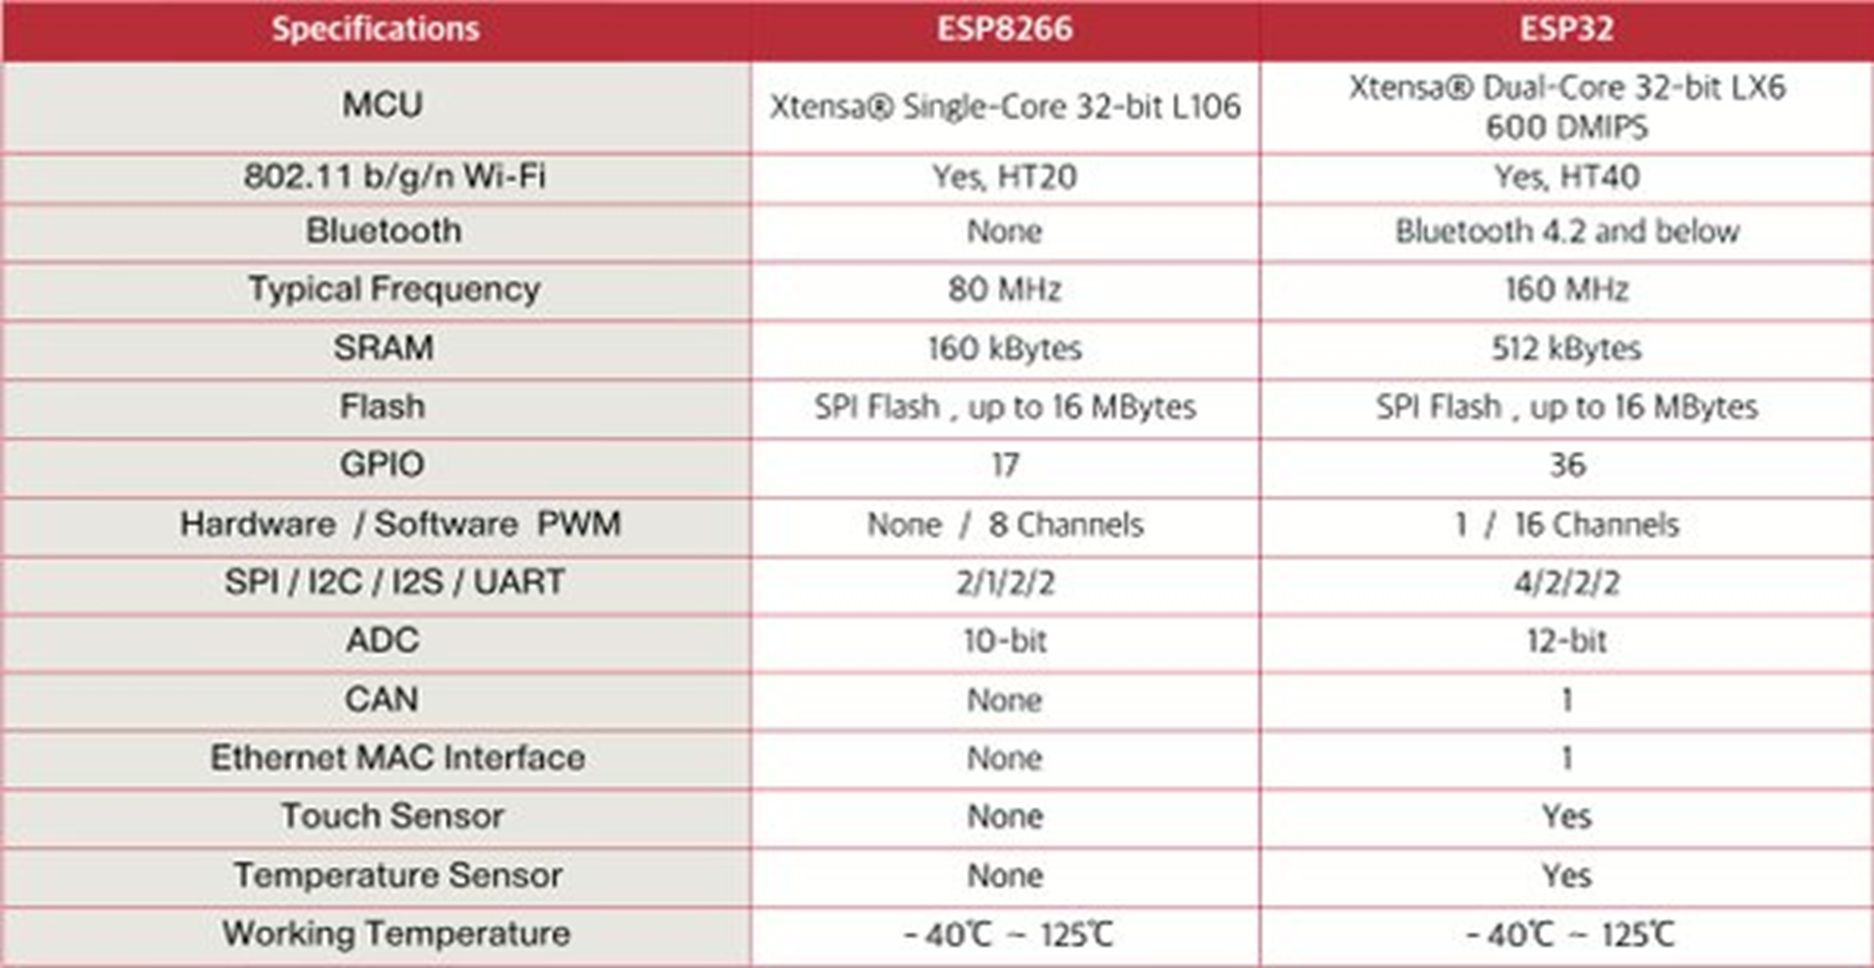
\includegraphics{obrazky/ESP.png}
	\caption{Srovnání specifikace modulů ESP8266 a ESP32. Převzato z \url{https://www.cnx-software.com/2016/03/25/esp8266-and-esp32-differences-in-one-single-table/}}
	\label{wifi-standards}
\end{figure}

\section{Python knihovny pro vývoj GUI}
K programování grafického uživatelského rozhraní existuje mnoho různých knihoven. Pro jazyk Python se nejčastěji používá některá z následujících knihoven:

\subsection*{Tkinter}

Knihovna tkinter je základní knihovna pro tvorbu okenních aplikací. Na rozdíl od ostatních knihoven je již obsažená v samotném jazyce Python, nemusí se tedy dodatečně instalovat [AL]. Používaní knihovny je tedy zdarma.\newline
Doporučuje se zvláště začátečníkům pro svou jednoduchost. Pro plnohodnotné využití je možné ke knihovně stáhnout dodatečné moduly [AM].

\subsection*{Kivy}

Knihovna Kivy patří mezi multiplatformní knihovny. Dle oficiálních stránek knihovny je možné vytvářet aplikace běžící na následujících zařízeních:

\begin{itemize}
    \item Desktopové počítače: OS X, Linux a Windows
    \item IOS zařízení: IPad a IPhone
    \item Android zařízení: tablety a telefony
    \item Jakékoli jiné dotykové zařízení, podporující TUIO (Tangible User Interface Objects) [AJ]
\end{itemize}

Knihovna přináší mnoho různých aspektů, které dle autorů knihovny mají zjednodušit tvorbu grafického rozhraní, obsluhu událostí a podobně.\newline
Ke knihovně rovněž patří zvláštní jazyk (nazvaný stejným jménem jako knihovna – jazyk Kivy). Jedním z jeho cílů je oddělení zodpovědnosti za prezentaci (zobrazení) a logiku programu [AK]. Zobrazení je dáno právě souborem kv (napsaném v jazyce Kivy) a logika souborem s Python kódem.\newline
Podobně jako tkinter, je i tato knihovna nabízena zdarma. Musí se však na rozdíl od tkinteru instalovat dodatečně.

\chapter{Zhodnocení současného stavu a plán práce}
V této kapitole se věnuji zhodnocení již existujících řešení automatizace domácnosti. Následně uvádím můj návrh řešení na základě nastudovaných řešení a vhodného rozsahu práce. Nakonec v bodech stanovuji cíle vyplývající z návrhu řešení, které se v práci snažím splnit.
\section{Současný stav}

Na trhu se v současné době nachází velké množství systémů. Z těch, které jsem popsal v části o existujících řešení je nejrozvinutějším systémem ten od společnosti Loxone. Zabírá opravdu širokou škálu možností a jen stěží by se hledala aplikace, pro kterou by nebyl vhodný. Kromě komplexnosti u něj oceňuji rovněž českou jazykovou lokalizaci. V češtině je k dispozici jak aplikace na ovládání (Loxone App), tak rovněž program pro konfiguraci systému (Loxone Config). Čím mě Loxone mile překvapilo je, že jsem si jejich aplikaci Loxone App mohl vyzkoušet v demoverzi i bez zakoupených komponent.\newline
Jako nevýhodu Loxone vidím příliš vysokou cenu. Uživatel, který si chce nainstalovat pár chytrých zařízení bude zřejmě překvapen cenou. Například při pořízení 3 chytrých zásuvek a miniserveru (který je k ovládání zásuvek potřebný) zaplatí přibližně 15 000 kč. Přitom adekvátní řešení od jiných firem, jako sonoff bude stát necelé 3000 kč, což je velký rozdíl – a při rozšiřování domácnosti o další prvky tento rozdíl znatelně roste. Na druhou stranu, pokud uživatel staví nový dům, může řešení od Loxone stát srovnatelnou cenu, jako konkurenční „neinteligentní“ instalace. Jako další nevýhodu vidím to, že celkově je instalace systému orientovaná spíše pro profesionální montáž pro pracovníky s příslušnou klasifikací (většina produktů je určena k zabudování do rozvaděče, příp. ke komunikaci s moduly v něm). Celkově je však řešení od Loxone na hodně vysoké úrovni.\newline

Řešení od firmy Jablotron je jistě zajímavé jejich dvoutlačítkovými (rozšiřitelnými) segmenty. Zdá se mi však nepraktické spojovat přístupovou klávesnici do domu s prvky automatizace domácnosti. Působí to poněkud omezeně. Navíc rozhraní pro ovládání domácnosti a alarmu v aplikaci MyJablotron se snaží napodobovat onu klávesnici, což příliš k přehlednosti nepřispívá. Na druhou stranu pro uživatele, jehož hlavní požadavek je zabezpečení objektu a pouze doplňková automatizace domácnosti (jako rozsvícení světel při odjištění domu) budou systémy od firmy Jablotron ideální.  \newline

Systém HomeKit je zajímavý v tom, že zde není potřeba žádný „speciální“ centrální prvek – pokud již uživatel vlastní například iPhone (či jiný produkt, který zastoupí funkci centrálního prvku). Nevýhodou je to, že aby byl systém ovladatelný globálně, tak je potřeba přeci jen mít v domácnosti nějaký prvek, co bude domácnost řídit. A pokud uživatel již nějaký nevlastní, tak se stává další investicí. Co je na systému HomeKit pozitivní je jeho nízká cena – ve srovnání se systémy od společnosti Loxone či Jablotron. Systém HomeKit se stále rozrůstá a má velkou podporu v rozmanitosti produktů. A na rozdíl od předchozích zmíněných systémů je více orientovaný na běžné uživatele. Jednou z nevýhod je zde to, že je systém orientovaný zejména na bezdrátovou komunikace, která samozřejmě někdy může být méně spolehlivá. Tím spíše že mnoho produktů komunikuje pouze pomocí Bluetooth, takže si uživatelé musejí hlídat dosah zařízení.\newline

Systém HomeConnect vnáší do automatizace domácnosti zajímavý koncept. Zatímco některé systémy umožňuji automatizovat domácnosti například chytrými zásuvkami či spínači, HomeConnect ve spolupráci s jinými společnostmi vyvíjí přímo spotřebiče s prvky chytré domácnosti, čímž tyto spotřebiče obsahují mnohem více „inteligence“, na rozdíl od pouhého „zapínání/vypínání“. Nicméně nevýhodou je zde příliš malý sortiment produktů, a tudíž jednoúčelová aplikace navíc, kterou stejně musejí uživatelé doplnit o další aplikace, chtějí-li například rovněž ovládat zásuvky, světla či rolety. Kromě toho je rovněž cena produktů dost vysoká.\newline
...

\section{Návrh řešení}
Na základě výzkumu dostupných řešení a jejich zhodnocení jsem se rozhodl vyvinout systém, který bude mít některé spíše základní funkce automatizace. Především zde bude řešeno dálkové ovládání jednoho zařízení druhým, jelikož je to zadání mé bakalářské práce. V systému tedy bude figurovat nějaký ovladač a dále ovládané prvky. 

V práci tudíž bude nutné zvolit vhodné vestavné zařízení, které bude sloužit jako ovládací část systému a také zařízení, která budou přijímat povely. Rozhodl jsem se, že ovládaný prvek zde nebude žádné konkrétní zařízení (jako zásuvka, spínač, či lampička) ale spíše nějaký obecný modul se vstupně výstupními porty, přes které bude možné ovládat jiná, už konkrétnější zařízení. Pro plnohodnotnou funkci systému bude tento modul nutné opatřit dalšími přídavnými součástkami. Půjde zejména o relé pro možnost ovládání zapnutí a vypnutí zařízení připojeného k tomuto modulu (tímto způsobem bude možné například ovládat LED pásek, či vytvořit bezdrátovou zásuvku). K modulu budou připojeny rovněž tranzistory pro možnost použití PWM modulace na výstupu - takový výstup pak bude sloužit pro stmívání světel, zejména LED pásku či bodových LED světel na 12 V. Ovládat tak bude možné rovněž servo motory, které se řídí PWM signálem.

Aby bylo ovládání systému co nejjednodušší, bude zde možnost ovládání na dotykovém displeji. Jelikož systém ovládaný jen z jednoho místa není v oblasti automatizace úplně nejšťastnějším a efektivním řešením (například uživatel sice nemusí dojít k vypínači světla, aby shasnul, ale stejně musí dojít někam k ovládacímu zařízení systému), rozhodl jsem se, že bude možnost ovládání i z telefonu, počítače a dalších zařízení (požadavky na zařízení budou definovaná později v části 6.X Návrh systému) \todo{Zmínit v implementaci požadavky}. Aby byl plněji využit potenciál displejů (ať už připojeného k ovládacímu zařízení, či ostatním zařízením, ze kterých bude možné moduly ovládat), rozhodl jsem se, že v systému bude možnost využívat několika různých senzorů.

Půjde o tyto senzory:
\begin{itemize}
    \item teploty
    \item pohybu
    \item sepnutí (kontaktu/tlačítka)
\end{itemize}
\todo{Uvést že dále budu ovládacímu zařízení říkat centrální prvek? Hub??}
Jde o typické představitele analogových i digitálních senzorů. Pro účely práce budou použity jen tyto tři, nicméně řešení chci pojmout jako open source (a s ohledem na tento fakt se budu snažit o co největší rozšiřitelnost systému), a další senzory bude možné přidat v budoucnu. Všechny senzory budou mít v systému pouze informativní charakter pro uživatele, tzn. bude si moci například zobrazit teplotu v konkrétní místnosti, zda se v ní někdo nachází, či zda byl sepnut nějaký kontakt (např. dveře). Nebude možné přímo systém pomocí senzorů ovládat, ale opět nic nebrání tomu, aby byla tato funkce implementována v budoucnu. U modulů s výhodou využiji, že budou mít více vstupů/výstupů a jeden modul tak může sdružovat více různých funkcí (například mít připojené 2 různé senzory a ovládat 5 výstupů).

Mým řešením bych chtěl doplnit existující open source řešení o takové, které bude svými vlastnostmi určeno spíše pro kutily v oblasti automatizace domácnosti. Bude poskytovat jednoduchý systém pro ovládání mnoha zařízení pomocí jednoho vestavného zařízení s připojeným displejem. Svou prací bych si chtěl rovněž vyzkoušet celý návrh a realizaci systému automatizace domácnosti, který bych následně mohl sám využívat. Vylepšením oproti některým již existujícím systémům bude možnost sdružení několika přijímajících zařízení do jednoho (jak jsem zmínil v předchozím odstavci).

Při práci budu využívat již existující moduly a mikropočítač (který bude sloužit jako „mozek“ systému), které však naprogramuji a vhodným způsobem doplním o některé elektronické součástky (jako zmíněné relé, či tranzistor). Práce se však nebude zabývat konstrukčním návrhem prvků systému, ani návrhem DPS pro hotový systém. Pro případně spojení komponent systému budou použita nepájivá kontaktní pole.

\section{Cíle práce}
Na základě předchozích úvah jsem se rozhodl, že vytvořím systém, který bude splňovat následující vlastnosti:

\begin{itemize}
    \item Bude zvolen vhodný mikropočítač, který bude sloužit jako ovládací část systému
    \item Pro ovládací část bude zvolen dotykový displej patřičných rozměrů, aby byl systém přehledný a mohl sloužit pro ovládání zařízení
    \item Displej by měl být rovněž vybrát s ohledem na možnost zobrazení přehledu o stavu zařízení v systému (například. zobrazení, které zařízení jsou zapnutá, či jaké hodnoty se nacházejí na PWM výstupu)
    \item K implementaci bude zvolen vhodný programovací jazyk
    \item Bude podporována funkce přímého ovládání výstupů ovládaných modulů
    \item Také zde bude funkce zobrazení dat ze senzorů
    \item Systém bude obsahovat českou jazykovou lokalizaci
    \item K systému bude možné přistupovat jak lokálně, tak i vzdáleně
    \item Pro vzdálený přístup zde budou fungovat uživatelské účty, přičemž z jednoho účtu bude možné ovládat jen jednu domácnost
    \item Bude zvolena vhodná technologie bezdrátového přenosu tak, aby byl systém co nejjednodušší na implementaci a případné rozšiřování
    \item Projekt bude uvolněn jako open source, čímž bude cena systému jako takového pro potenciální uživatele minimální (daná pouze cenou použitých součástek a zařízení)
\end{itemize}

\chapter{Realizace a testování}
V této kapitole se věnuji vlastní realizaci řešení a následnému testování a vyhodnocení. V první podkapitole uvádím celkový návrh systému -tedy z jakých aplikací a zařízení se bude skládat, jak mezi sebou budou komunikovat apod. Následně se věnuji návrhu grafického uživatelského rozhraní pro aplikaci, ke kterým uživatel bude přistupovat. V dalších kapitolách již rozebírám implementaci konkrétních aplikací. Nakonec uvádím jak jsem systém testoval a k jakým výsledkům testy vedly.
\todo{Někde vymezit pojmy...klient, klientská aplikace, (koncový) modul...}
\section{Celkový návrh systému}
Systém se bude skládat celkem ze tří aplikací a několika zařízení (každé zde bude mít svou roli). 

\subsection*{Zařízení}
Jmenovitě budou v systému fungovat tato zařízení:
\begin{itemize}
    \item Centrální jednotka (s připojeným displejem)
    \item Koncové moduly
    \item Senzory
    \item Ovládaná zařízení
    \item Ostatní zařízení, přes která bude možné systém ovládat (klienti)
\end{itemize}

Centrální jednotka bude mít na starosti celý systém řídit. Pokud například uživatel zadá pokyn ke změně hodnoty na některém výstupu modulu, bude to právě Centrální jednotka, kdo tuto žádost (v jistém smyslu) přijme a pošle ji dále jako příkaz na konkrétní koncový modul.
Jelikož k centrální jednotce bude potřeba připojit (dotykový) displej, musí mít dostatečný výkon pro vykreslování na něj a zpracování dat. Bylo tedy potřeba zvolit vhodný mikropočítač (protože mikrokontrolery mívají obecně daleko menší výkon) opatřený nějakým portem pro přenos obrazu. Jedním z nejpoužívanějším a také nejrychleji vyvíjejícím se mikropočítačem je Raspberry Pi, vlastní ho tedy již mnoho IT\todo{?} nadšenců. Je relativně levné (ve verzi 3 se dá sehnat do jednoho tisíce kč, verzi Zero W je dokonce možné na českém trhu sehnat za přibližně 300 kč) a tedy i snadno dostupné. Nadto je použití Raspberry Pi doporučeno v zadání mé práce.

Koncový modul (dále již jen modul) bude zařízení, které bude mít nějaké vstupy a výstupy. Modul bude měnit hodnoty na svých výstupech dle instrukcí, přicházejících z centrální jednotky. K těmto výstupů pak budou dále připojeny příslušné součástky (jako relé, či tranzistor) a k nim dále již reálná zařízení, ve kterých budou nějakým způsobem spínat kontakt. Rovněž bude v pravidelných intervalech číst hodnoty na svých vstupech (ke kterým budou připojeny senzory). Jako koncový modul je potřeba vybrat zařízení s nízkou cenou, jelikož těchto zařízení může být i více. Kromě toho bude modul přijímat pouze jednoduché příkazy od Raspberry Pi, může se tedy klidně jednat o nějaký mikrokontroler s omezeným výpočetním výkonem. Je však potřeba, aby byl tento mikrokontroler schopný komunikovat po síti (tento požadavek vyplývá ze zadání mé bakalářské práce). Na trhu existují především 2 takové mikrokontrolery - ESP8266 a novější ESP32.

Ovládanými zařízeními zde myslím ta, co budou připojena na některý z výstupů modulu. Půjde tedy například o LED pásek, či zařízení, u kterého bude spínat kontakt.

Klientská zařízení budou libovolná zařízení, přes které bude uživatel moci ovládat systém. Jedinými požadavky na tato zařízení jsou zde vzhledem k implementaci:
\begin{itemize}
    \item Přístup k internetu
    \item Dostatečně velký displej (ideálně 5´´ a více)
\end{itemize}

\subsection*{Aplikace}
Dále kromě zařízení budou v systému fungovat tyto tři aplikace:
\begin{itemize}
    \item Klientská aplikace (dále již jen klient), určená jako grafické rozhraní pro uživatele k ovládání systému
    \item Server, který bude od klienta (ať už přímo, nebo zprostředkovaně skrze databázi) získávat instrukce a vykonávat je
    \item Aplikace na modulech
\end{itemize}

Po úvaze jsem dospěl k názoru, že nejvhodnější bude, když bude klient implementován jako jednostránková webová aplikace. A to z několika důvodů:
\begin{itemize}
    \item Webové aplikace jsou obecně vzato multiplatformní (pokud mají alespoň trochu responzivní design), čehož vhodně využiji v rámci možnosti ovládat domácnost i na dálku
    \item K přístupu k aplikaci tak bude stačit mít zařízení s přístupem k internetu (a obrazovkou pochopitelně)
    \item Webové technologie patří mezi rychle se rozvíjející, což přispívá k budoucímu rozvoji systému
    \item Jazyk Typescript (který budu používat) je jeden z vůbec nejpoužívanějších a nejznámějších programovacích jazyků, pokud se tedy najde programátor, který by chtěl v budoucnu systém rozšířit, je velká pravděpodobnost se nebude muset učit nic nového.
\end{itemize}

\begin{figure}[!hbt]
	\centering
	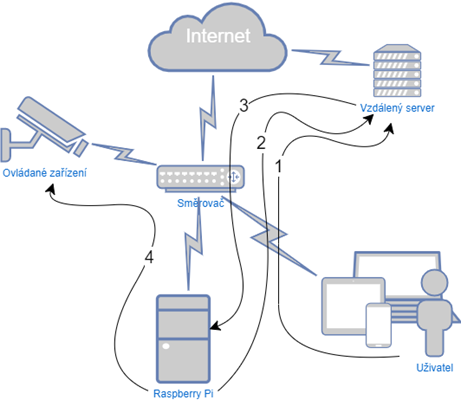
\includegraphics[scale=0.7]{obrazky/architektura.png}
	\caption{Architektura systému pro automatizaci domácnosti}
	\label{architektura}
\end{figure}
\todo{Upravit scale obrázku výše!}

Druhá aplikace pak bude běžet na Raspberry Pi jako server zpracující požadavky jednak od klientů, a pak také samozřejmě požadavky zadané přímo na displeji Raspberry Pi \todo{...rozvést...}


Jako alternativu těchto prvních dvou aplikací bylo možné vytvořit jen jednu, běžící na Raspberry Pi, přes kterou by se systém ovládal pouze z připojeného displeje. Nicméně tímto by se ztratila možnost ovládat systém i vzdáleně, resp. i z jiných zařízení, než je Raspberry Pi, což by bylo jistě neintuitivní a mnohdy nepříjemné, zvolil jsem tedy řešení dvou aplikací.

\subsection*{Programové prostředky}
\todo{Vysvětlit proč jsem si vybral zrovna typescript a node.js a jaké jsou alternativy (a alternativní řešení)}

\subsection*{Celková architektura systému}
\todo{Uvést celkově co s čím a jak bude komunikovat, dle obrázku \ref{architektura} (a vytvořit nový)}

Na obrázku \ref{architektura} je možné vidět celkovou koncepci systému.


\section{Grafický návrh klientské aplikace}
Aplikace byla rozdělena na několik samostatných částí (oken), mezi kterými může uživatel přecházet. Jelikož se jedná o jedno stránkovou aplikaci, nejde v případě jednotlivých částí o klasické stránky (v tom smyslu, že by každá měla vlastní html dokument, který ji generuje). V následujícím textu se však budu odkazovat ke každému takovému samostatnému oknu, jako k jedné (webové) stránce.
\subsection*{Přihlašovací stránka a registrace}
Na úvod při spuštění se zobrazí stránka, na které se uživatel bude moci přihlásit (pomocí emailu a hesla). Rovněž zde bude možnost přejít k registraci nového účtu, vyžádat si zapomenuté heslo či projít dále do aplikace bez přihlášení (tato možnost bude pouze v aplikaci Raspberry Pi).

\subsection*{Menu}
V aplikaci se přihlášenému uživateli bude zobrazovat vyjíždějící menu, kterým se bude moci přepínat mezi jednotlivými stránkami (jako domovská stránka či nastavení). V menu také bude možnost odhlášení, která však pravděpodobně nebude často využívána.
\subsection*{Domovská stránka}
Za domovskou stránku považuji tu, na kterou se uživatel dostane ihned po přihlášení do systému. Tato stránka bude sloužit i jako výchozí pro ovládání jednotlivých zařízení. Bude zde také přehled hodnot na senzorech. Tuto stránku bude mít uživatel zobrazenou většinu času na displeji Raspberry Pi, pokud jej bude chtít používat jako takový rychlý přehled o stavech ovládaných zařízení (a senzorech).
Jak vidíme na obrázku XYm bude tato stránka rozvržena na jednotlivé místnosti. Pro každou zde bude pod sebou vyhrazené místo a v něm pro každou místnost se stejným rozvržením - název místnosti, seznam hodnot na senzorech a ovládaná zařízení (ze kterých bude možné vyčíst jejich stav i ovládat je). Pokud bude chtít uživatel ovládat nějaké zařízení, klikne na něj. V případě zařízení typu zapnuto/vypnuto se okamžitě změní stav zařízení. V případě zařízení, řízených PWM modulací se zobrazí nad zařízeními posuvník (nastavený na aktuální hodnotu), kterým bude možné okamžitě měnit hodnotu na výstupu modulu (a tedy stav zařízení).

\subsection*{Nastavení}
V aplikaci bude také stránka s nastavením. Bude zde možnost přidávat nová zařízení a konfigurovat ta stávající...
\todo{Dodělat...Nebude zde nastavení a konfigurace zvlášť?}


\section{Implementace klientské aplikace}
\todo{Zmínit že spárování uživ. účtu s RPi bude tím, že se přihlásí uživatel na lokálním serveru}
\section{Implementace serveru na Raspberri Pi}
\section{Implementace aplikace pro koncové moduly}
\section{Testování a vyhodnocení systému}


\subsection*{Provedené testy}
V rámci testování jsem provedl tyto testy:
\begin{itemize}
    \item Test reaktivity
    \item Test intuitivnosti uživatelského prostředí
    \item Test stability při potížemi s připojením k internetu
    \item Test autonomie?
\end{itemize}

Test reaktivity (neboli odezvy systému na podněty v reálném čase) probíhal takto...

Test intuitivnosti uživatelského prostředí probíhal takto...

Test Test stability při potížemi s připojením k internetu probíhal takto...

Test autonomie (funkce systému bez lidského zásahu) probíhal takto...

\subsection*{Testy které nebyli provedeny}
Kromě testů, které jsem už provedl by bylo vhodné provést ještě dále zmíněné. V případě absence prvních dvou nedojde k žádným potížím (jen systém možná nebude fungovat na jiných zařízeních). Problémy, které by se otestovali zbylými dvěma testy by však mohli být kritické. Alespoň u čtvrtého testu ale věřím, že nejsou obavy na místě, přeci jen je konkurence velká a systém by neměl být zahlcený. V rámci mé práce tyto testy vykonány nebyli, zejména z finančních a časových důvodů.
Testy které by bylo vhodné provést:
\begin{itemize}
    \item Funkčnost systému na alternativních mikropočítačích 
    \item Funkčnost systému na jiných verzích Raspberry Pi
    \item Stabilita systému v průběhu několika let chodu
    \item Test spolehlivosti systému při velkém množství uživatelů
\end{itemize}
Raspberry Pi je jedním z nejpoužívanějších a nejznámějších mikroprocesorů, nicméně na trhu se nacházejí další, u kterých by bylo vhodné otestovat, zda bude server i klientská aplikace (na připojeném displeji) plně funkční. Zejména mikropočítače uvedené v kapitole \ref{vestavne-systemy} (tam jsem totiž popisoval rovněž nejpopulárnější mikropočítače)

Funkčnost systému na jiných verzích Raspberry Pi je potřeba otestovat zejména z toho důvodu, že se jedná o poměrně rychle se rozvíjející platformu a někteří potenciální uživatelé tak mohou mít starší model s nižším výkonem. Zvláště zajímavý by byl test na verzi Zero W, jelikož tuto verzi Raspberry Pi je možné pořídit za přibližně 300 kč. V případě bezproblémového chodu by byl projekt velmi zajímavou alternativou k některým velmi drahým systémům jako je \todo{XYZ}. Je možné, že by například nebyla tato verze Raspberry Pi dostatečně výkoná na ovládání systému z připojeného displeje, ale zvládala by na běh aplikace serveru, pak by bylo možné systém prostě ovládat z klientů (například chytrých telefonů). Případně kdyby tato verze nezvládala bezproblémový běh serveru s poskytováním statické stránky, tak by bylo možné tuto část serveru upravit (odstranit) a pak by se klienti připojovali pouze na vzdálený server a úloha Raspberry Pi by se zredukovala pouze na kontrolu (resp. naslouchání) změn v databázi a komunikaci s koncovými moduly, což by snad mělo opravdu bez jakýchkoli potíží fungovat. Pak by se samozřejmě muselo vyřešit spárování Raspberry Pi s uživatelským účtem, protože aktuálně to funguje právě na principu, který vyžaduje, aby se uživatel (alespoň poprvé) přihlásil na poskytované statické stránce z Raspberry Pi.

Test stability systému by pak spočíval v tom, že by systém pravidelně po dobu několika let využívalo jisté množství lidí (například 100 domácností) a pozorovalo, zda se systém v průběhu času chová stále stejně, nezpomaluje se a podobně.

Test spolehlivosti systému při velkém množství uživatelů by bylo provést hlavně z toho důvodu, že v systému funguje jedna veřejná databáze. Vylo by vhodné otestovat, jak se systém bude chovat při velké zátěži databáze (ve chvíli, kdy bude k databázi aktivně současně přistupovat mnoho uživatelů).






























\chapter{Závěr}
\label{zaver}

Nápady na pokračování práce:
\begin{itemize}
    \item ovládání hlasem
    \item přidání podmínek
    \item přidání módů (scén) - v podstatě by se jednalo o sdružení více akcí ovládání do jedné
    \item vývoj by mohl směřovat i na odlehčení serveru tak, že bude pouze kontrolovat databázi a komunikovat s moduly (jak bylo polemizováno v testování) => a mohla by se vytvořit verze pro ESP8266 v režimu Centrální jednotky => velice levný systém...
\end{itemize}

Moje odkazy \cite{4technologie} \cite{BezdratoveSite} \cite{DesigningEmbeddedSystems} \cite{EmbeddedSystems}
\cite{EmbeddedSystemsCircuits}
\cite{ITURegulations} \cite{MicroprocessorAndInterfaces} \cite{WifiFrequencyBands} \cite{uCvsCPU} \cite{arduino} \cite{ArduinoProgramming} \cite{whatIsIR} \cite{optics} \cite{physics} \cite{HomeAutomationRPI} \cite{Everything2_4GHZ} \cite{microwave} \cite{materials} \cite{wirelessComunication} \cite{NetworkSecurity} \cite{RPiPrirucka} \cite{BluetoothGuide} \cite{WirelessPersonalCommunications} \cite{GettingStartedBluetooth} \cite{Why2_4GHz} \cite{ESP8266} \cite{ESP32} \cite{HandsOnZigBee} \cite{ZigbeeWirelessNetworking}


%===============================================================================

  \fi
  
  % Kompilace po částech (viz výše, nutno odkomentovat)
  % Compilation piecewise (see above, it is necessary to uncomment it)
  %\subfile{projekt-01-uvod-introduction}
  
  %\subfile{chapters/projekt-05-conclusion}


  % Pouzita literatura / Bibliography
  % ----------------------------------------------
\ifslovak
  \makeatletter
  \def\@openbib@code{\addcontentsline{toc}{chapter}{Literatúra}}
  \makeatother
  \bibliographystyle{bib-styles/Pysny/skplain}
\else
  \ifczech
    \makeatletter
    \def\@openbib@code{\addcontentsline{toc}{chapter}{Literatura}}
    \makeatother
    \bibliographystyle{bib-styles/Pysny/czplain}
  \else 
    \makeatletter
    \def\@openbib@code{\addcontentsline{toc}{chapter}{Bibliography}}
    \makeatother
    \bibliographystyle{bib-styles/Pysny/enplain}
  %  \bibliographystyle{alpha}
  \fi
\fi
  \begin{flushleft}
  \bibliography{projekt-20-literatura-bibliography}
  \end{flushleft}

  % vynechani stranky v oboustrannem rezimu
  % Skip the page in the two-sided mode
  \iftwoside
    \cleardoublepage
  \fi

  % Prilohy / Appendices
  % ---------------------------------------------
  \appendix
\ifczech
  \renewcommand{\appendixpagename}{Přílohy}
  \renewcommand{\appendixtocname}{Přílohy}
  \renewcommand{\appendixname}{Příloha}
\fi
\ifslovak
  \renewcommand{\appendixpagename}{Prílohy}
  \renewcommand{\appendixtocname}{Prílohy}
  \renewcommand{\appendixname}{Príloha}
\fi
%  \appendixpage

% vynechani stranky v oboustrannem rezimu
% Skip the page in the two-sided mode
%\iftwoside
%  \cleardoublepage
%\fi
  
\ifslovak
%  \section*{Zoznam príloh}
%  \addcontentsline{toc}{section}{Zoznam príloh}
\else
  \ifczech
%    \section*{Seznam příloh}
%    \addcontentsline{toc}{section}{Seznam příloh}
  \else
%    \section*{List of Appendices}
%    \addcontentsline{toc}{section}{List of Appendices}
  \fi
\fi
  \startcontents[chapters]
  \setlength{\parskip}{0pt} 
  % seznam příloh / list of appendices
  % \printcontents[chapters]{l}{0}{\setcounter{tocdepth}{2}}
  
  \ifODSAZ
    \setlength{\parskip}{0.5\bigskipamount}
  \else
    \setlength{\parskip}{0pt}
  \fi
  
  % vynechani stranky v oboustrannem rezimu
  \iftwoside
    \cleardoublepage
  \fi
  
  % Přílohy / Appendices
  \ifenglish
    %\input{projekt-30-prilohy-appendices-en}
  \else
    \chapter{Obsah přiloženého paměťového média}

\begin{itemize}
    \item doc - Složka obsahující text technické zprávy a jeho zdrojový kód.
    \item src - složka zdrojových kódů. Obsahuje podsložky:
        \begin{itemize}
            \item analyzer - Složka obsahující skripty pro trénování analyzátorů a následnou analýzu.
            \item bash\_scripts - Skripty ke spouštění.
            \item downloader - Složka se skripty pro stahování recenzí ze zdrojových webů.
            \item helper\_scripts - Pomocné skripty.
            \item sentiment\_analytics - Webové rozhraní implementované v aplikačním rámci \emph{Django}.
        \end{itemize}
    \item plakat.pdf - Plakát.
    \item readme.txt - Textový soubor popisující postup instalace systému.
\end{itemize}                   
  \fi
  
  % Kompilace po částech (viz výše, nutno odkomentovat)
  % Compilation piecewise (see above, it is necessary to uncomment it)
  %\subfile{projekt-30-prilohy-appendices}
  
\end{document}
